% vim: tw=80

\chapter{Measurement of the Triple-Differential Dijet Cross Section}

\section{Datasets}
\label{sec:datasets}

\subsection{Data Samples}

Within the run 1 of the data-taking at the LHC, the CMS experiment collected in
2012 data at a center-of-mass energy of $\sqrt{s} = 8 \si{\TeV}$. The data
sample corresponds to a total integrated luminosity of $\mathcal{L} = 19.71
\si{\fbinv}$. The events are streamed into different primary datasets based on
the trigger decision. All data triggering the prescaled or unprescaled jet
triggers were assigned to the \texttt{JetMon} or \texttt{JetHT} primary
datasets, respectively. The datasets are split into multiple samples
corresponding to the period of data taking in 2012, called Run A,B,C and D.
Unfortunately the trigger assignment to the primary datasets changed during the
data taking period, as can been seen in Table~\ref{tab:data:datasets}, it was taken
care to avoid any double counting. While in run A all events were stored in the
dataset \texttt{Jet}, the prescaled and unprescaled triggers were split into
separate streams \texttt{JetMon} and \texttt{JetHT} in the runs B, C and D.

\begin{table}[htbp]
    \centering
    \begin{tabular}{llll}
    \toprule
    Run & Run Range & Dataset & Luminosity (\si{\fbinv})\\\midrule
    A & 190456--193621 & /Jet/Run2012A-22Jan2013-v1/AOD & 0.88\\
    B & 193834--196531 & /Jet[Mon,HT]/Run2012B-22Jan2013-v1/AOD & 4.49\\
    C & 198022--203742 & /Jet[Mon,HT]/Run2012C-22Jan2013-v1/AOD & 7.06 \\
    D & 203777--208686 & /Jet[Mon,HT]/Run2012C-22Jan2013-v1/AOD & 7.37\\ 
    \bottomrule
    \end{tabular}
    \caption{The full 2012 dataset is used. In Run A, events of all single jet
        trigger paths are stored in the stream \texttt{Jet}, while the prescaled
        triggers were moved to the \texttt{JetMon} stream in the runs B, C and
        D. Events triggering the unprescaled trigger are collected in the data
        stream \texttt{JetHT}.}
    \label{tab:data:datasets}
\end{table}

\subsection{Monte Carlo Samples}

To compare the data distributions with simulated events, two Monte-Carlo event
generators were considered. An overview about the Monte-Carlo generators is
given in Section~\ref{subsection:mc_generators}. Each MC generator is using and
optimized tune to simulate the underlying event. Additionally the data samples
contain not only the hard interaction but also a model for pile-up collionsion,
through which additional soft scattering events following the pile-up
distribution in data are mixed into the event.

The Madgraph+P6 sample is a multi-leg improved HT-binned sample. By using
Madgraph, the LO matrix elements not only contain the $2 \rightarrow 2$ matrix
elements, but also the $2 \rightarrow 3$ matrix elements better describing
multijet events. The underlying event is modelled using the tune $Z2*$. The
parton shower and hadronization is carried out using the Pythia 6 event
generator which is interfaced to Madgraph using the LHE event record.

Additionally a Pythia 8 data sample is analyzed. While including only the $2
\rightarrow 2$ LO matrix elements, the event simulation and the underlying event
tune are improved in this newer Pythia version. Both Monte-Carlo samples are
processed through the complete CMS detector simulation to allow studies of the
detector response and compare to the measured data on detector level. 

\begin{table}[htp]
    \centering
    \begin{tabular}{llll}
    \toprule
    Dataset Name & Dataset identifier & Number of events\\\midrule
    MG+P6 &
    \makecell{/QCD\_HT-XXToXX\_TuneZ2star\_8TeV-madgraph-pythia/\\ Summer12\_DR53X-PU\_S10\_START53\_V7A-v1/AODSIM} & \\
    P8 & \makecell{QCD\_Pt-XXtoXX\_Tune4C\_8TeV\_pythia8/\\
    Summer12\_DR53X-PU\_S10\_START53\_V7A-v1/AODSIM} & \\
    \bottomrule
    \end{tabular}
    \caption{Official MC production samples used in the analysis.}
    \label{tab:montecarlo:datasets}
\end{table}

Since the jet spectra steeply fall with increasing \pt it is not possible to
generate a high number of high-\pt events in a reasonable time.  Therefore the
event generation is split into different phase space region binned in HT, the
scalar sum of the jet \pt, or the leading jet \pt. The different phase space
regions are then stitched together later in the data analyses while taking into
account the cross section in the different phase space regions.
Table~\ref{tab:montecarlo:datasets} shows the used data sets and the number of
events per dataset.

\section{Event selection}

\subsection{Certified Data Selection}

The first step in the event processing chain is to only pick runs and
luminosity sections (LS) which fullfill certain criteria. These include the
proper performance of all detector subsystem and the passing of the data quality
monitoring (DQM) steps during the validation process. The good lumisections
within a run are then announced using a JSON data file, called \textit{Golden
JSON}. The applied lumi certification file in our analysis is based on the final
event reconstruction of the 2012 datasets.

\begin{verbatim}
Cert_190456-208686_8TeV_22Jan2013ReReco_Collisions12_JSON.txt
\end{verbatim}

\subsection{Trigger Selection}

To measure and reconstruct the \ptavg spectrum of the dijet production, a set of
single jet triggers have been used. Single jet triggers consist of one L1
trigger seed and multiple HLT filters. The L1 trigger has a smaller threshold to
ensure full efficiency versus \pt for the HLT trigger. Table~\ref{tab:triggers}
shows the full set of single jet triggers employed. Since the \pt spectrum is
exponentially falling and the rates for low-\pt jets are very high, it is not
possible to use a single unprescaled trigger to select all interesting events.
Therefore a set of prescaled low-\pt triggers each with different prescales is
used to collect sufficient data in the lower part of the \pt spectrum.
Additionally one unprescaled trigger is used in the region where the jet rate is
sufficiently small to collect all events. The prescales are taken into account
again when the spectrum is reconstructed. 

\begin{table}[htbp]
    \centering
    \begin{tabular}{lcccr}
        \toprule
        Trigger path  & L1 (\si{\GeV}) & HLT (\si{\GeV}) & $p_{\mathrm{T},.99\%}$ (\si{\GeV}) & Eff. Lumi \\\midrule
        HLT\_PFJet40  & 16                  & 40                   & --                     & 0.08 \si{\pbinv}\\
        HLT\_PFJet80  & 36                  & 80                   & 123                    & 2.12 \si{\pbinv}\\
        HLT\_PFJet140 & 68                  & 140                  & 192                    & 55.67 \si{\pbinv}\\
        HLT\_PFJet200 & 92                  & 200                  & 263                    & 0.26 \si{\si{\fbinv}}\\
        HLT\_PFJet260 & 128                 & 260                  & 353                    & 1.06 \si{\si{\fbinv}}\\
        HLT\_PFJet320 & 128                 & 320                  & 412                    & 19.71 \si{\si{\fbinv}}\\
        \bottomrule
    \end{tabular}
    \caption{Used trigger paths in the analysis. Each path is used in an mutually exclusive phase space in \ptavg. The
            $p_{\mathrm{T},.99\%}$ threshold gives the value at which a trigger reaches 99\% efficiency compared to lower
            reference trigger.}

    \label{tab:triggers}
\end{table}


\begin{figure}[htbp]
    \centering
    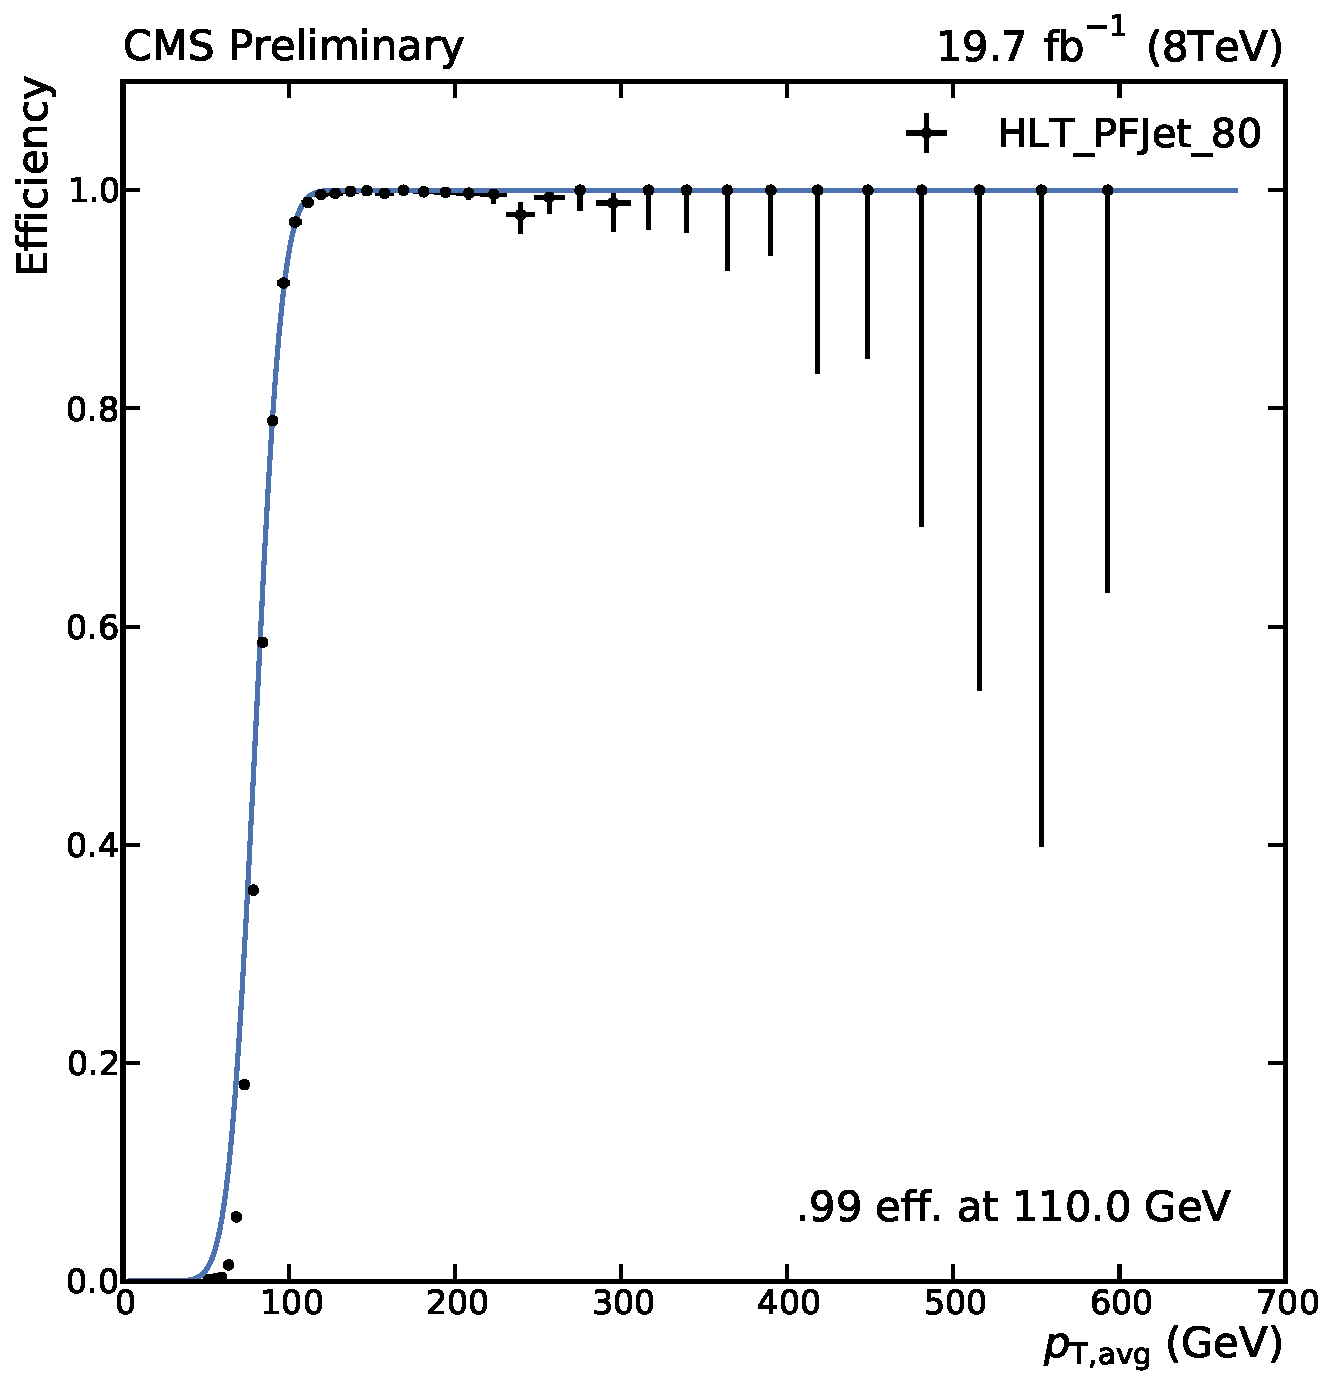
\includegraphics[width=0.45\textwidth]{figures/measurement/trigger_eff_hltpfjet80.pdf}\hfill
    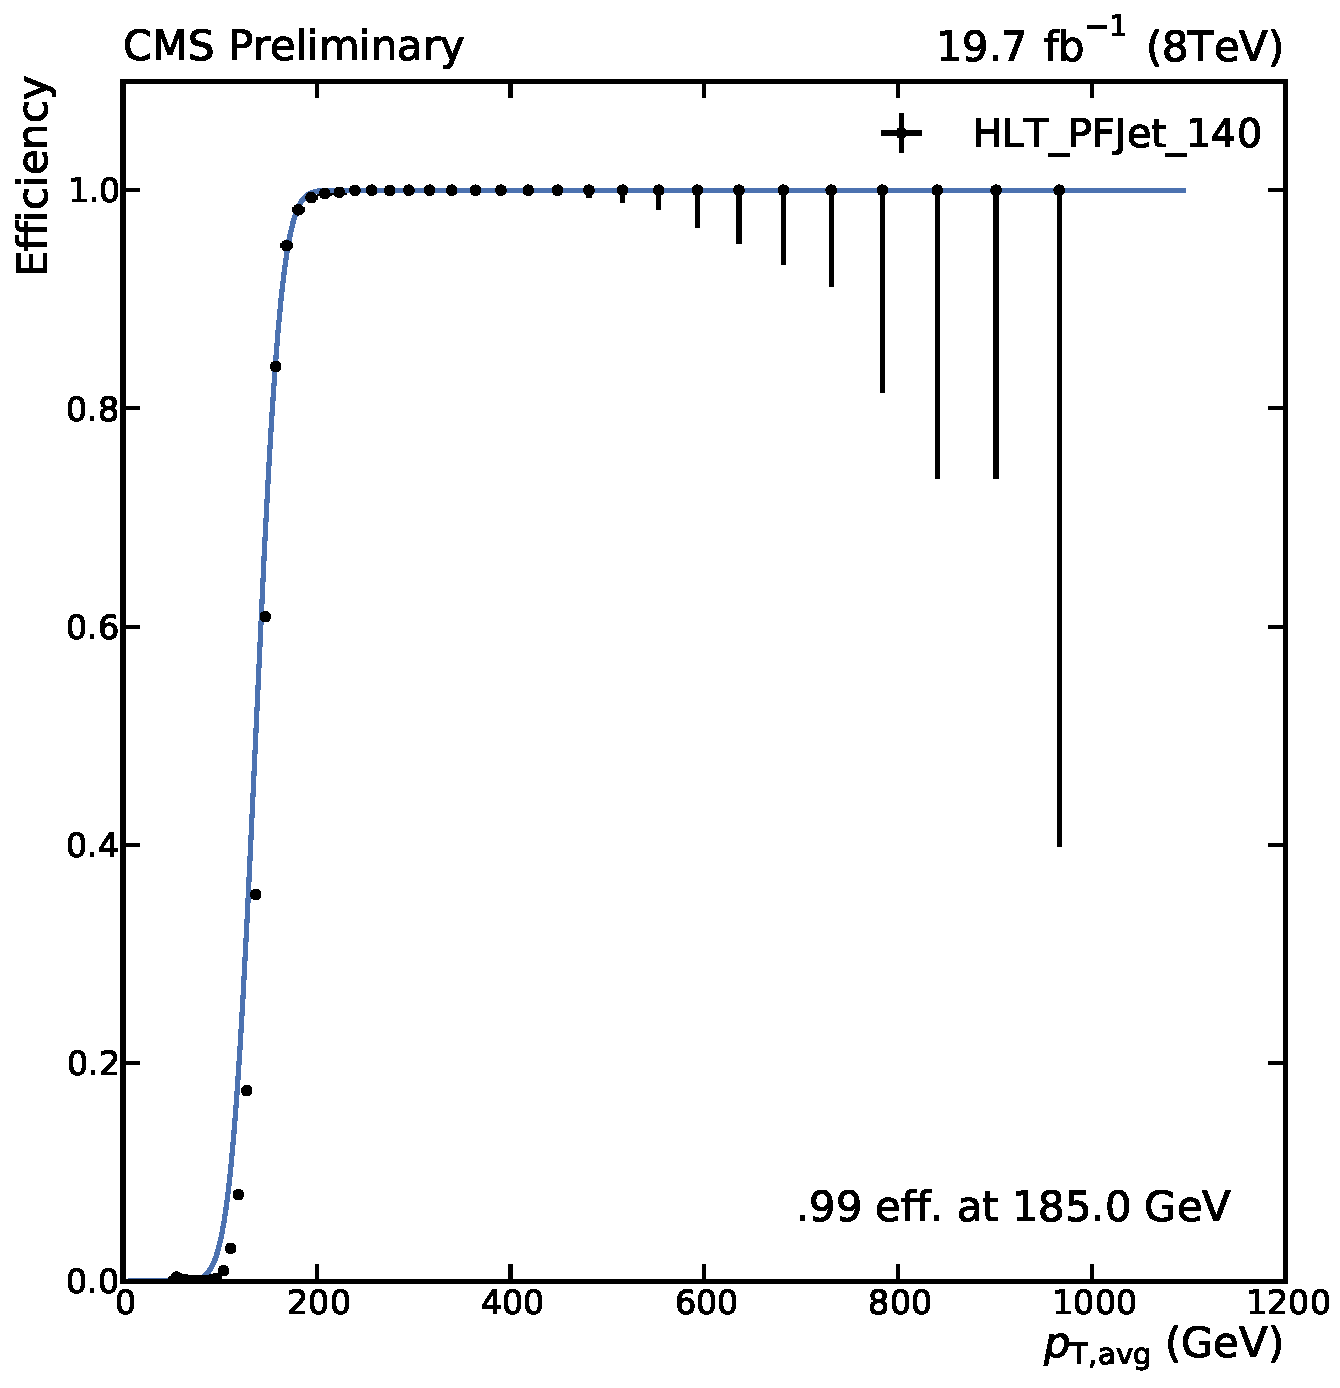
\includegraphics[width=0.45\textwidth]{figures/measurement/trigger_eff_hltpfjet140.pdf}
    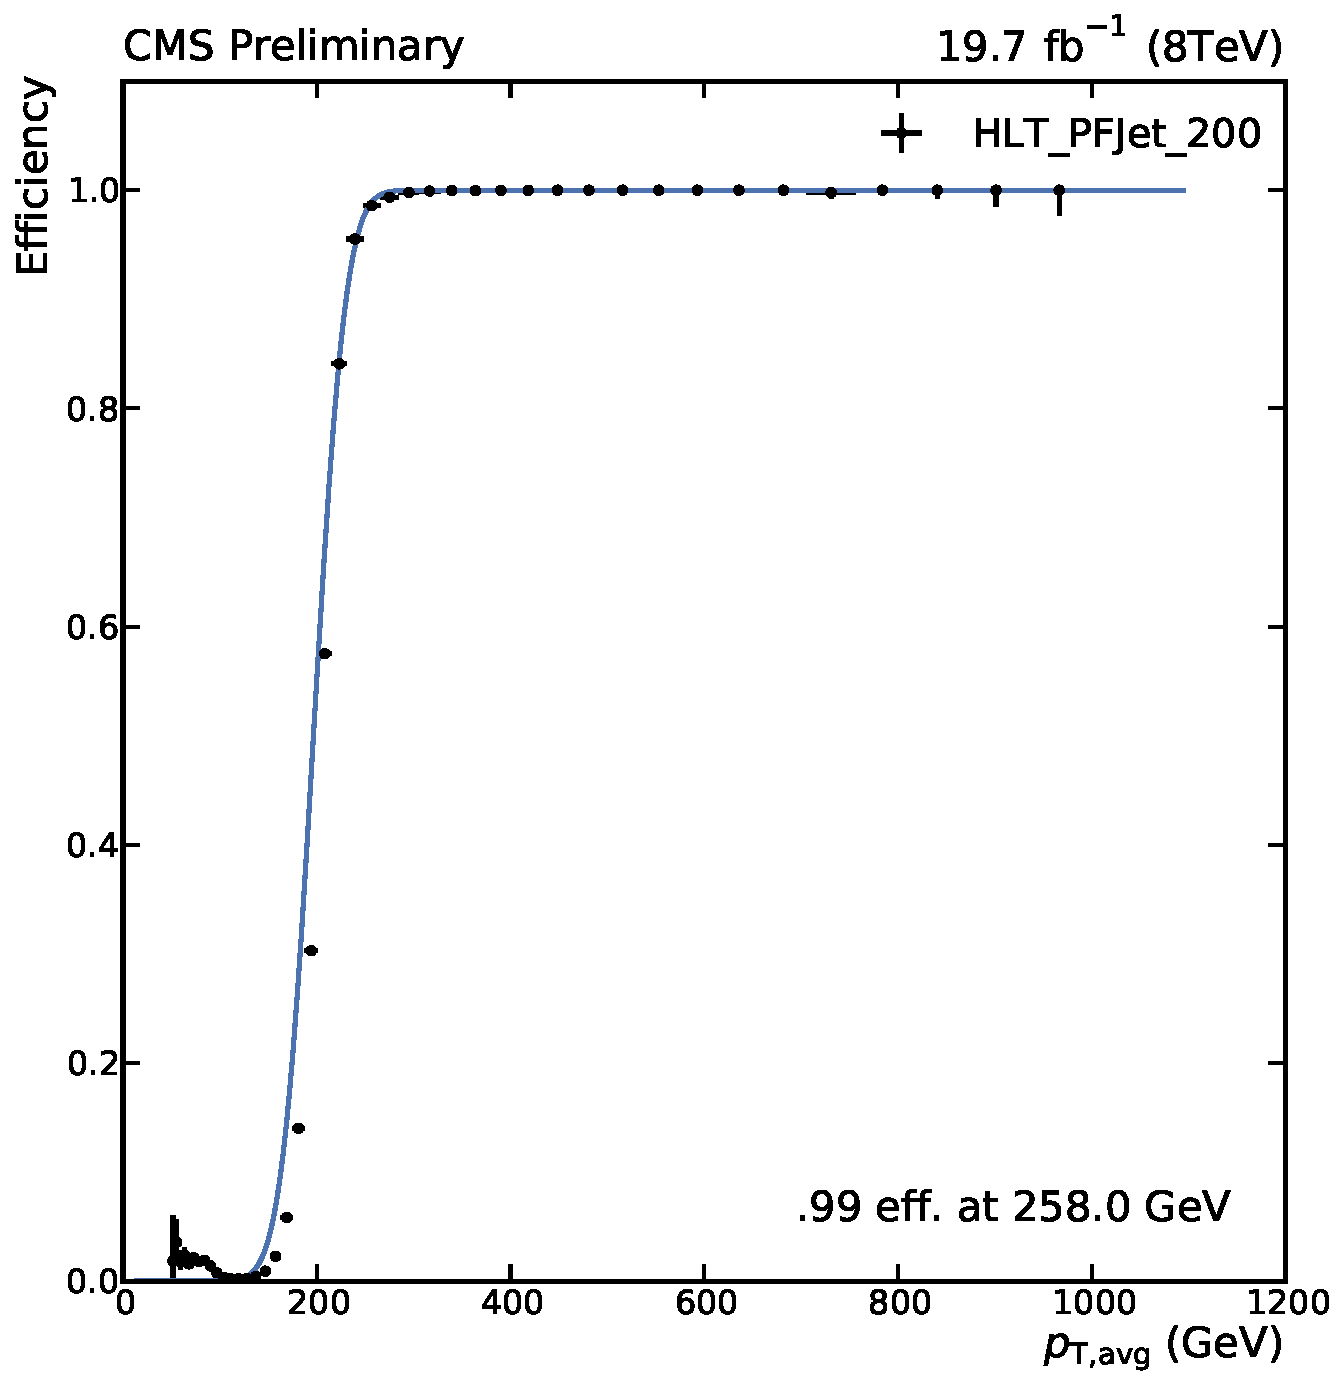
\includegraphics[width=0.45\textwidth]{figures/measurement/trigger_eff_hltpfjet200.pdf}\hfill
    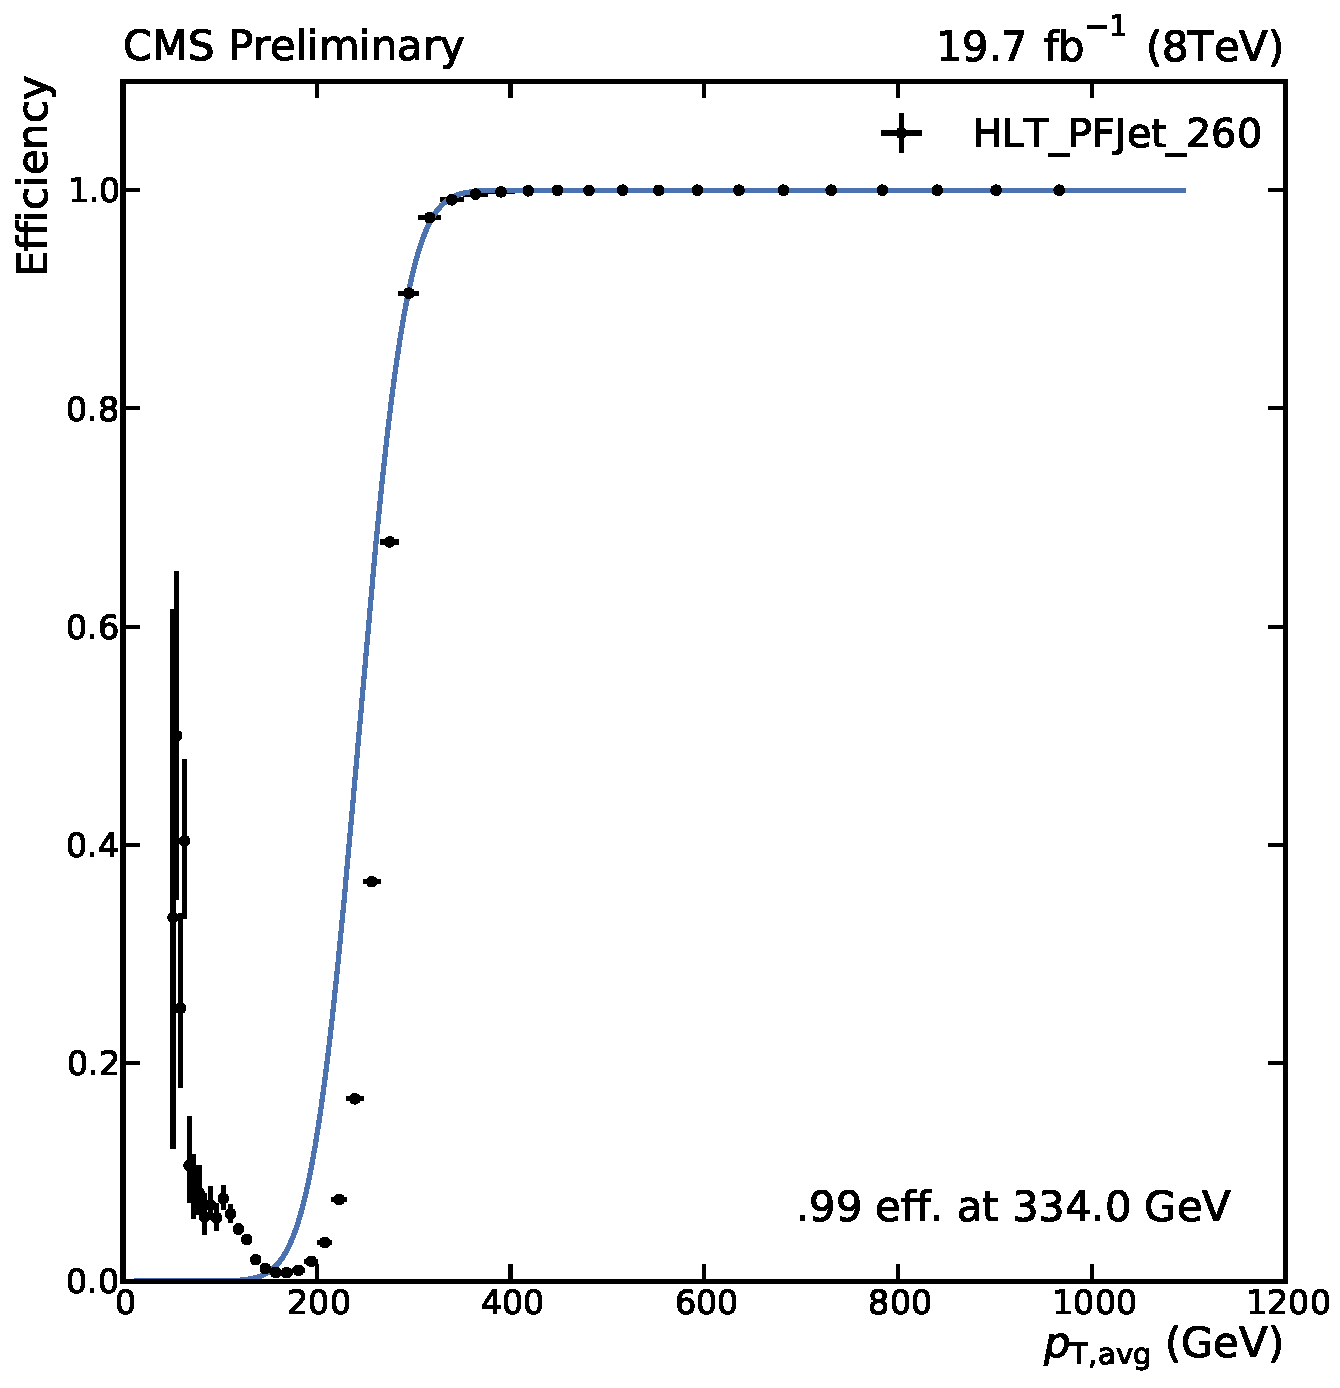
\includegraphics[width=0.45\textwidth]{figures/measurement/trigger_eff_hltpfjet260.pdf}
    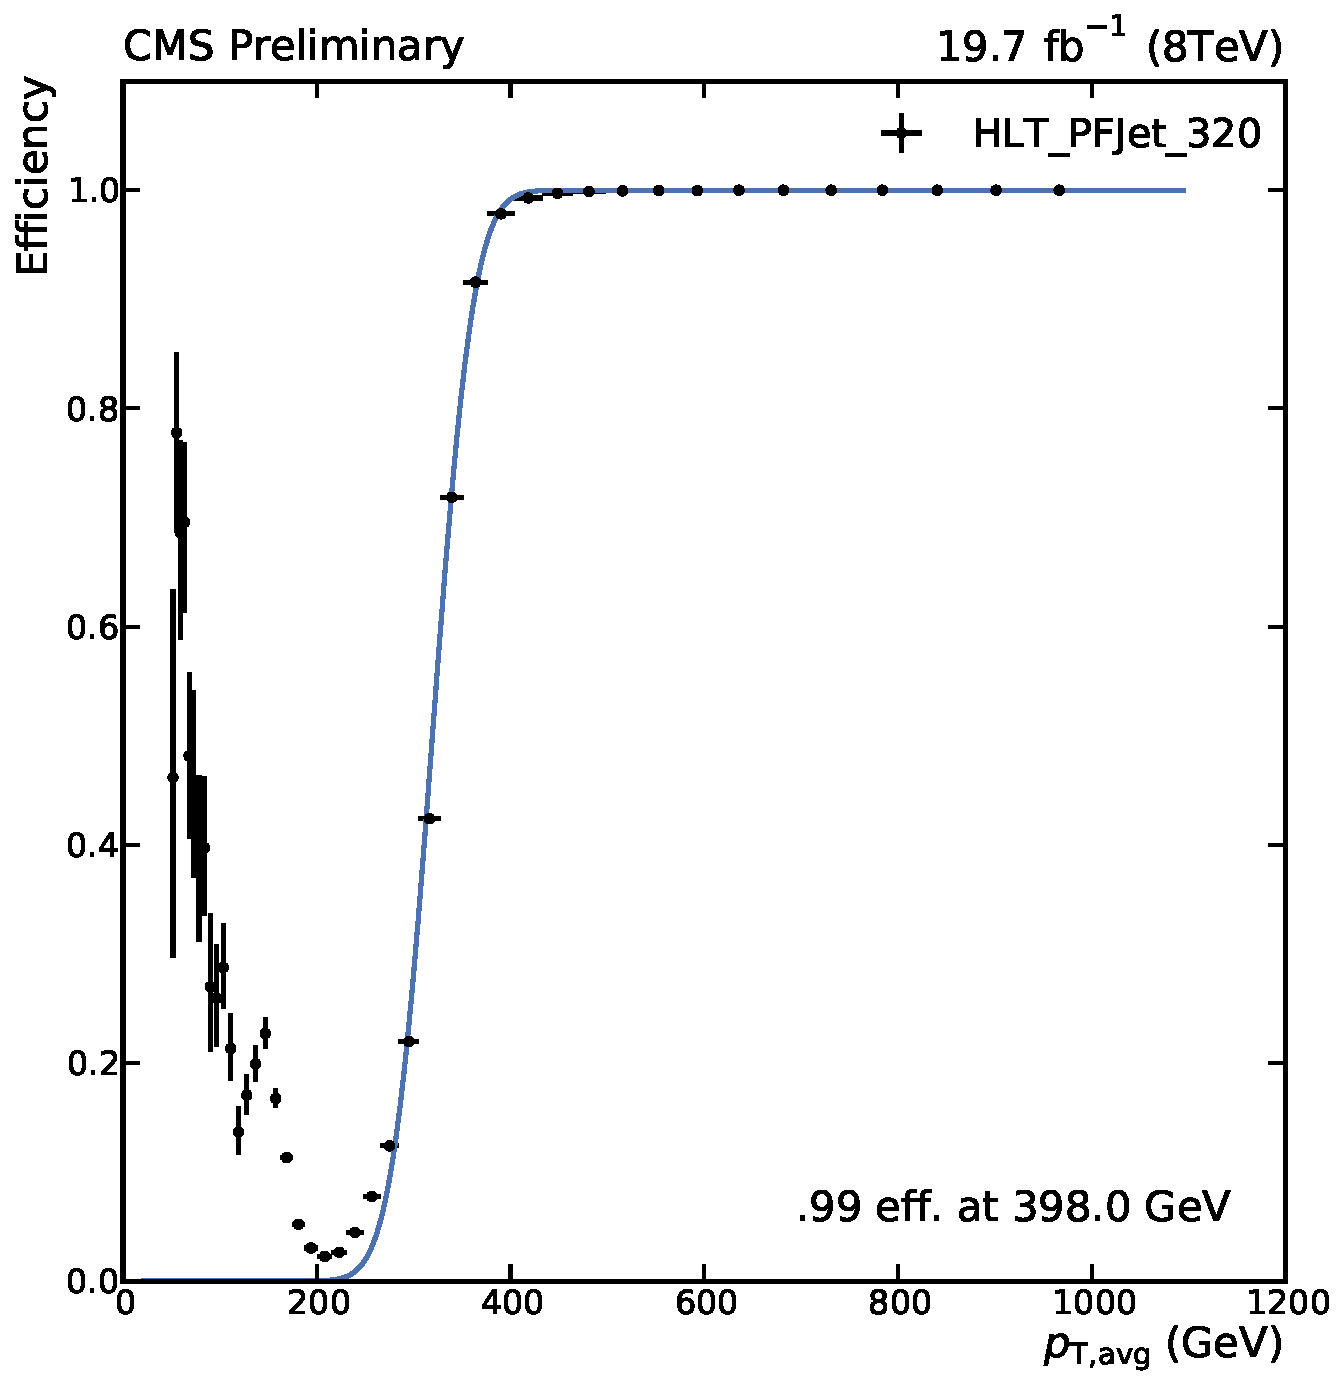
\includegraphics[width=0.45\textwidth]{figures/measurement/trigger_eff_hltpfjet320.pdf}\hfill
    \caption{Trigger efficiencies turn-on curves for the single jet trigger
    paths used in the analysis. To determine the 99\% efficiency threshold, the
    trigger paths are fitted using a sigmoid function taking into account the
    uncertainties using Clopper-Pearson confidence intervals.}
    \label{fig:trigger_eff}
\end{figure}

The reconstruction algorithms and the jet energy corrections applied on HLT
level are slightly different compared to the final data reconstruction.
Additionally the trigger efficiency is not calculated versus $\ptjet$ which was
used in the trigger decision, but versus the \ptavg of the dijet system used in
this analyses. Therefore the trigger paths show a turn-on behaviour as can been seen in
Figure~\ref{fig:trigger_eff} and it is neccessary to determine the threshold at
which a trigger is fully efficient.

Due to the different prescales introduced by each trigger path, it is not
trivially possible to calculate the efficiency by dividing the number of passed events for
one trigger by dividing through the number of events passed by the previous
trigger with the lower \pt threshold which is by definition fully efficient for
the higher trigger path. While it is possible to normalize the yield by the
effective luminosity seen by each trigger, this introduces statistical
fluctuations due to the large differences of the number of events seen by each
trigger caused by the prescale factors.

When the L1 trigger and HLT trigger are processed, the objects passing the
trigger are stored. Therefore it is possible to re-emulate the trigger decision
by comparing the L1 jet \pt with the L1 trigger threshold and the HLT jet \pt
with the HLT threshold~\cite{Stober:2012abc}.

Similarly the trigger decision of the next higher jet trigger can be emulated
starting from the lower trigger path. A set of events $S_1 = \left\{E_i | T_A
(E_i) = true \right\}$ which was accepted  by the lower trigger path $T_A$ is
used to determine the subset $S_2 = \left\{E_i|T_A(E_i) \wedge  T_B(E_i)
\right\}$ which would also pass the higher trigger $T_B$. The ratio of both
event sets can be used to determine the efficiency as shown for each trigger
path in Figure~\ref{fig:trigger_eff} using the Equation~\ref{eq:trigger_eff}.
The error bars of the trigger efficiency are given by Clopper-Pearson confidence
intervals.

\begin{equation}
\label{eq:trigger_eff}
    f_{\mathrm{eff}} (x) = \frac{N(\left\{E_i|T_A(E_i) \wedge T_B(E_i), x)\right\}}{N(\left\{ E_i | T_A(E_i) = \mathrm{true} \right\} , x)}
\end{equation}

The efficiency versus \ptavg is fitted using the sigmoid function~\ref{eq:trigger_eff_fit} describing
the turn-on behaviour of the trigger paths. Each trigger was used in a region in which the efficiency
is larger than $99\%$. The actual used trigger efficiency deviate slightly from the once shown in Table~\ref{tab:triggers}
since the used trigger eff. thresholds were measured for each \ystar and \yboost bin and the most
conservative value was used.

\begin{equation}
\label{eq:trigger_eff_fit}
    f_{\mathrm{fit}} (x) = \frac{1}{2} \left( 1 + \erf \left(\frac{x-\mu}{\sqrt{2}\sigma}\right)\right)
\end{equation}

Table~\ref{tab:triggers} contains the L1 and HLT thresholds of each trigger and
the \ptavg value at which each trigger reaches 99\% efficiency.

\subsection{Primary Vertex Selection}

The \textbf{good primary vertex selection} further rejects beam background and off-centre bunch
crossings. The recommended vertex selection cuts ensure at least one well
reconstructed primary vertex for an event to be further analyzed. The following
criteria are applied 

% Vertex selection
% To reject further beam backgrounds and off-centre parasitic bunch crossings,
% the recommended vertex selection cuts are applied. To pass the step of the
% selection process, an event has to contain at least one well reconstructed
% primary vertex (PV), within a distance of |z(PV)| < 24 cm between the pri-
% mary vertex and the nominal interaction point (IP) of the detector. The
% radial distance ρ(PV) of the vertex from the z axis though the IP is required
% to be smaller than 2 cm, corresponding to the size of the beam pipe. Addi-
% tionally, the fit used to determine the vertex needs to have P
% at least 4 degrees
% of freedom. For an unconstrained vertex fit, which has 2 i w i − 3 degrees
% of freedom (w i ≤ 1), this means at least four tracks with weight ≈ 1 are
% required. The influence of the different steps of the vertex selection is shown
% in table 6.5.

\subsection{Missing transverse energy cuts}

If all particles could be identified and perfectly measured, the sum of the
transverse momenta would sum up to zero. The imbalance in the transverse
momentum of all visible particles, which can be measured in the detector, is
called the missing transverse momentum (MET). Neutrinos, for example, leave the
detector undetected and do contribute to the MET. MET is an important ingredient
in many measurements involving W bosons, top quarks or searches for physics
beyond the standard model which involve undetectable particles. 

A large fraction of the MET is not always caused by physics processes. Very
often the reason can be found in detector noise, cosmic rays or beam-halo
particles. Therefore there are a sequence of algorithms developed by the MET
working group at CMS identifying and rejecting these events. Additionally a cut
was introduced which removes events in which the missing transverse energy
fraction \met constitutes a large fraction of the total transverse energy.

\begin{equation}
    \frac{\met}{\sum_i E_{T,i}} < 0.3
\end{equation}

\subsection{Jet ID selection}

The jet identification criteria rejects noise and noise-enhanced
jets while keeping all real jets. The jet ID is not applied event-wise, but each
jet is accecpted or rejected by the jet id selection. The algorithm works on
particle flow jets using information of the underlying particles. 
Following the recommendations the official loose jet ID is used. Each jet
passing the jet id criteria is then further processed in the analysis chain. The
jet id criteria are based on the properties of each jet. The properties and the
respective cuts are listed in Table~\ref{tab:jetid}. The cut on the neutral
hadron and electromagnetic fractions removes HCAL and ECAL noise. Muons which
are falsely identified and clustered as jets are removed by the muon fraction
criterion. Based on information of the tracker, additional selection cuts are
enforced in the region $|\eta| < 2.4$. Fake jets clustered from electrons are
removed by the charged electromagnetic fraction cut and the charged hadron
fraction must be larger than zero.

While studying the loose and tight jet criteria, it was found that the tight jet
id removes a non-negligible fraction of jets in the forward region of the
phase space considered in this analysis. Therefore the loose jet id was applied.

\begin{table}[htbp]
    \centering
    \begin{tabular}{llll}
    \toprule
                           & Property                & Loose ID & Tight ID\\\cmidrule(lr){2-4}
    Whole $\eta$ region    &                         &          & \\\cmidrule(lr){1-1}
                           & Neutral Hadron Fraction & $< 0.99$ & $< 0.90$\\
                           & Neutral EM Fraction     & $< 0.99$ & $< 0.90$\\
                           & Number of Constituents  & $> 1$    & $> 1$\\
                           & Muon Fraction           & $< 0.8$  & $< 0.80$\\
    Only $|\eta| < 2.4$    &                         &          & \\\cmidrule(lr){1-1}
                           & Charged Hadron Fraction & $> 0$    & $> 0$\\
                           & Charged Multiplicity    & $> 0$    & $> 0$\\
                           & Charged EM Fraction     & $< 0.99$ & $< 0.90$\\
    \bottomrule
    \end{tabular}
    \caption{The jet identification criteria remove fake jets originating from
    detector noise as well as wrongly clustered electrons and muons. Following
    the official recipe, the loose jet id was applied.}
    \label{tab:jetid}
\end{table}

\subsection{Jet Corrections}

Following the latest recommendations of the JERC group, the jet energy corrections \texttt{Winter14 V8}
and the corresponding uncertainty files were used for data, while the \texttt{START53\_V27} uncertainties
for run-independent MC were applied on the MC samples.

\subsection{Phase space cuts}

% jet 1/2 rapidity < 3.0
% jet1 pt > 133 GeV
% jet2 pt > 50 GeV

Several cuts in the phase space of the dijet system are applied to select a
clean phase space region as shown in Table~\ref{tab:jetcuts}. 

\begin{table}[htbp]
    \centering
    \begin{tabular}{llll}
    \toprule
                    & |y|     & \pt (GeV)\\\midrule
    Leading jet     & $< 3.0$ & 74.\\
    Second jet      & $< 3.0$ & 50\\
    \bottomrule
    \end{tabular}
    \caption{The selection cuts applied on the leading and second jet in the
    event. }
    \label{tab:jetcuts}
\end{table}

The rapidity selection restricts the measurement to a phase space region without
detector inefficencies. In case the leading or second jet has a rapidity higher
than 3.0, the whole event is rejected. The first and second jet each have
different transverse momentum cuts to avoid infrared sensitivity of the NLO
theory calculation.

Effectively there is also a cut on the average \pt of the dijet system
introduced by the trigger thresholds. Since the first trigger is only fully efficient
at 133 GeV, the spectrum is only measured above this value. This also avoid any
turn-on regions of the spectrum which are difficult to model in the unfolding
procedure.

If there are not at least two jets in the event fullfilling these criteria, the
whole event is rejected.

\section{Comparison with Simulated Events}

\subsection{Comparison of Kinematic Quantities}

The measured data distributions on detector level are compared with simulated events
processed through the whole event generation and detector simulation. In this section
the basic kinematic quantities of the leading two jets are compared as well as the properties
of each of the jets mainly describing the constituent fractions of each jet. Figure~\ref{fig:controlplots:kinematic}
shows the transverse momentum $\pt$, the rapidity $y$ and the azimuthal angle $\phi$ for the leading
two jets. The kinematic of the two dijet system is well described by the MC simulation apart from
a few regions with larger discrepancies. The \pt-distribution is not that well described escpecially in
the lower \pt region and the number of events with forward jets is overestimated in the MC simulation.

\begin{figure}[htbp]
    \centering
    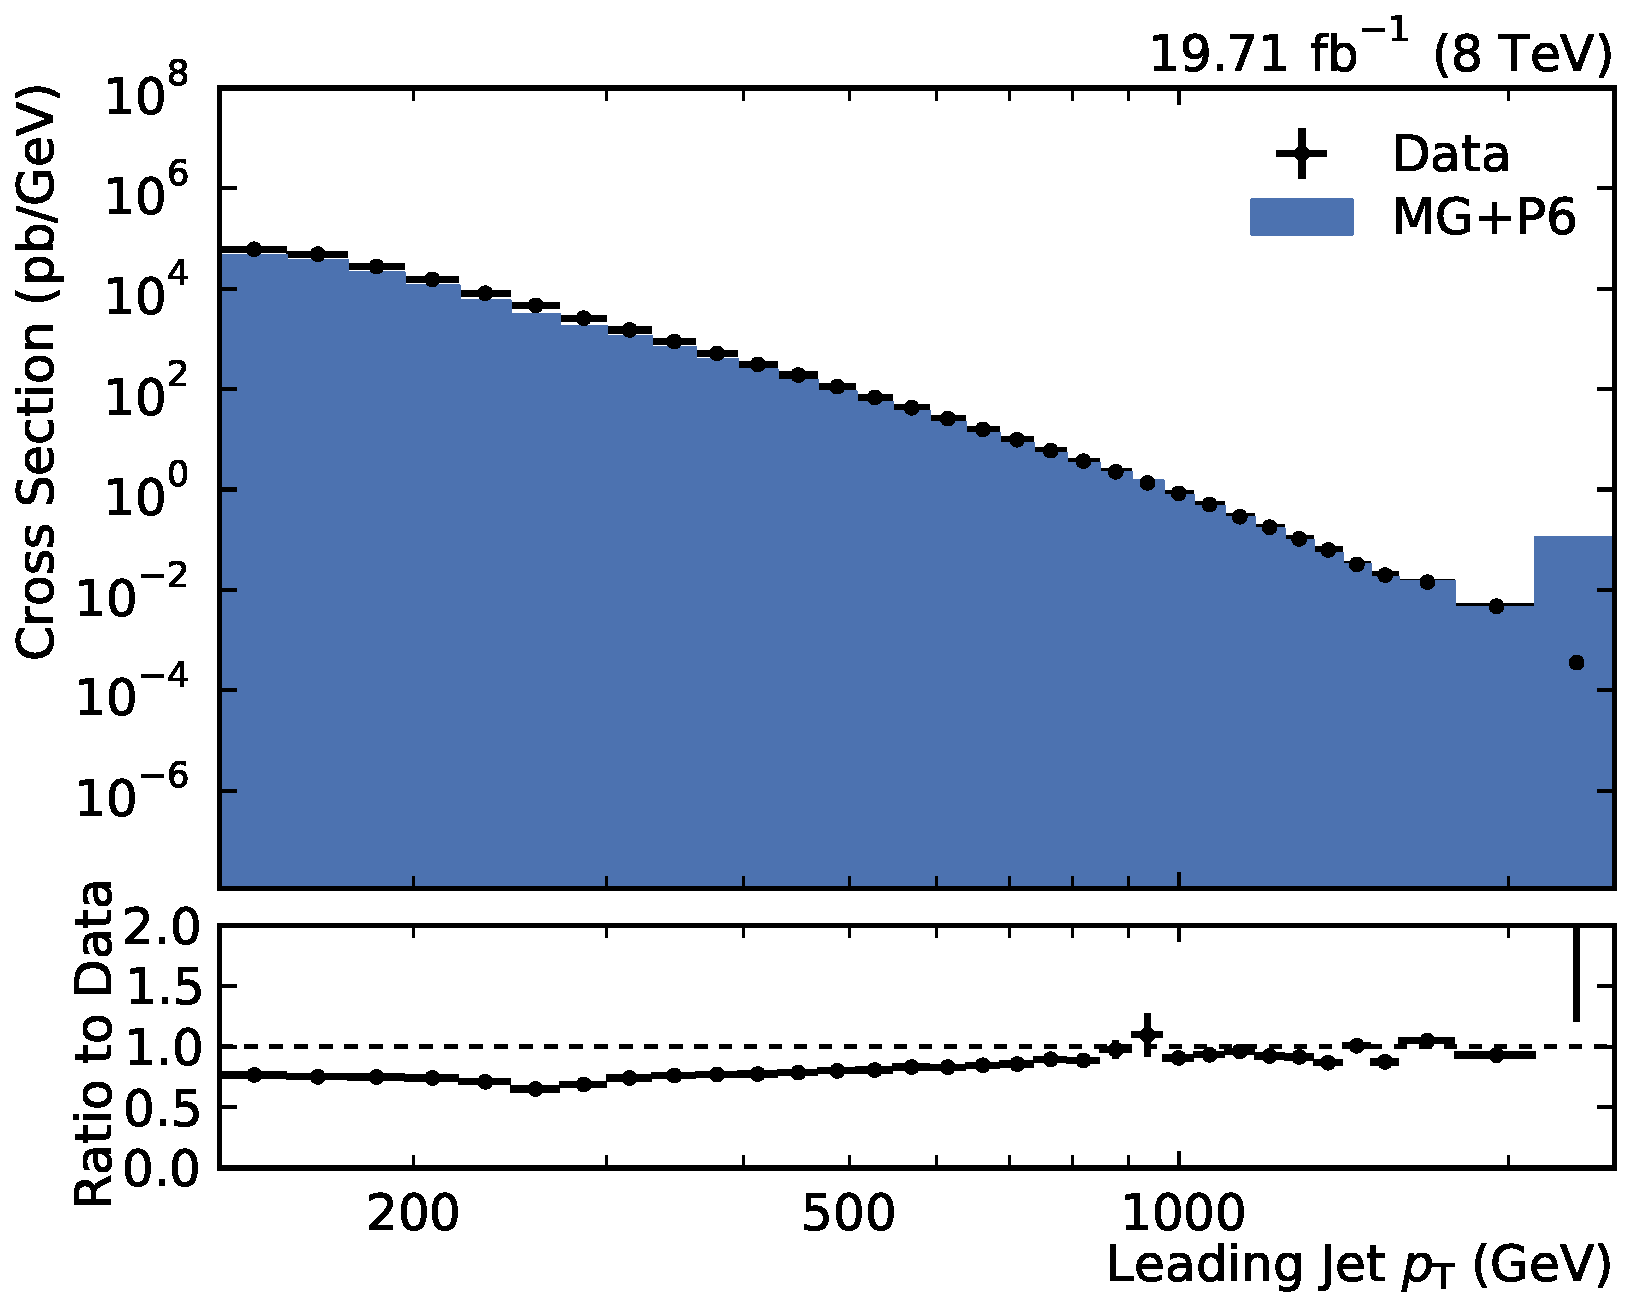
\includegraphics[width=0.45\textwidth]{figures/measurement/jet1pt_default.pdf}\hfill
    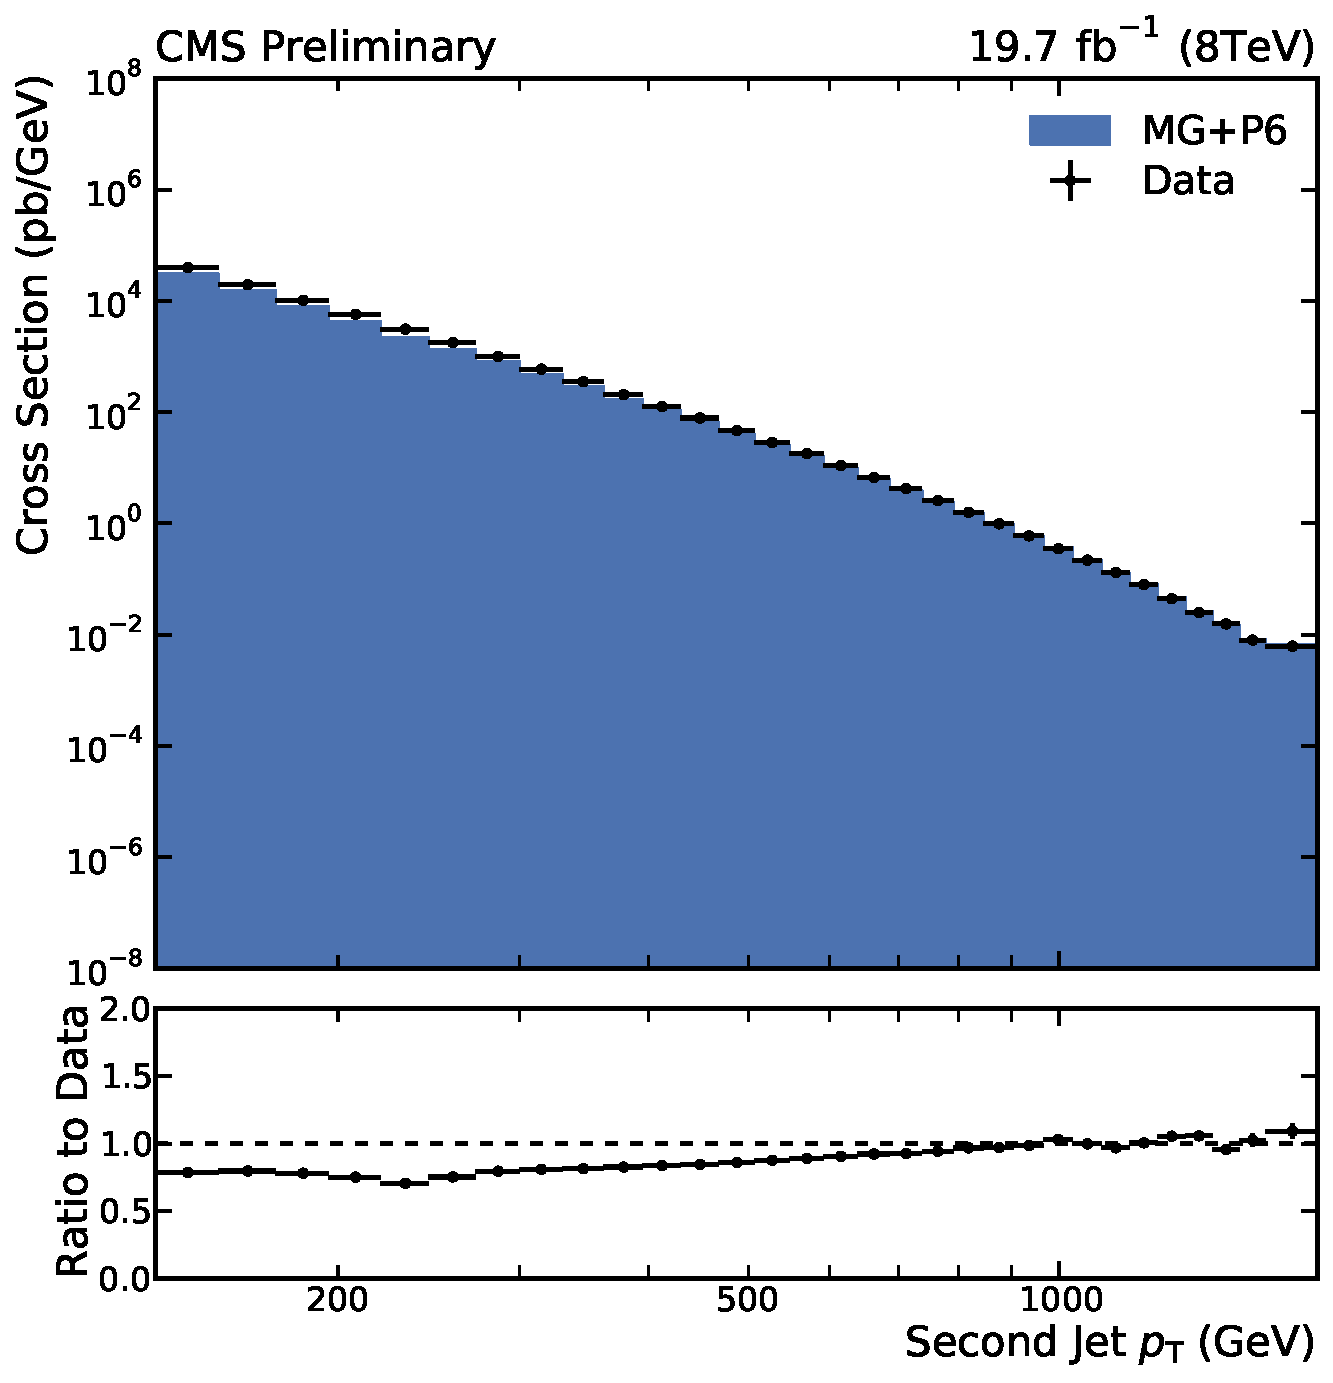
\includegraphics[width=0.45\textwidth]{figures/measurement/jet2pt_default.pdf}
    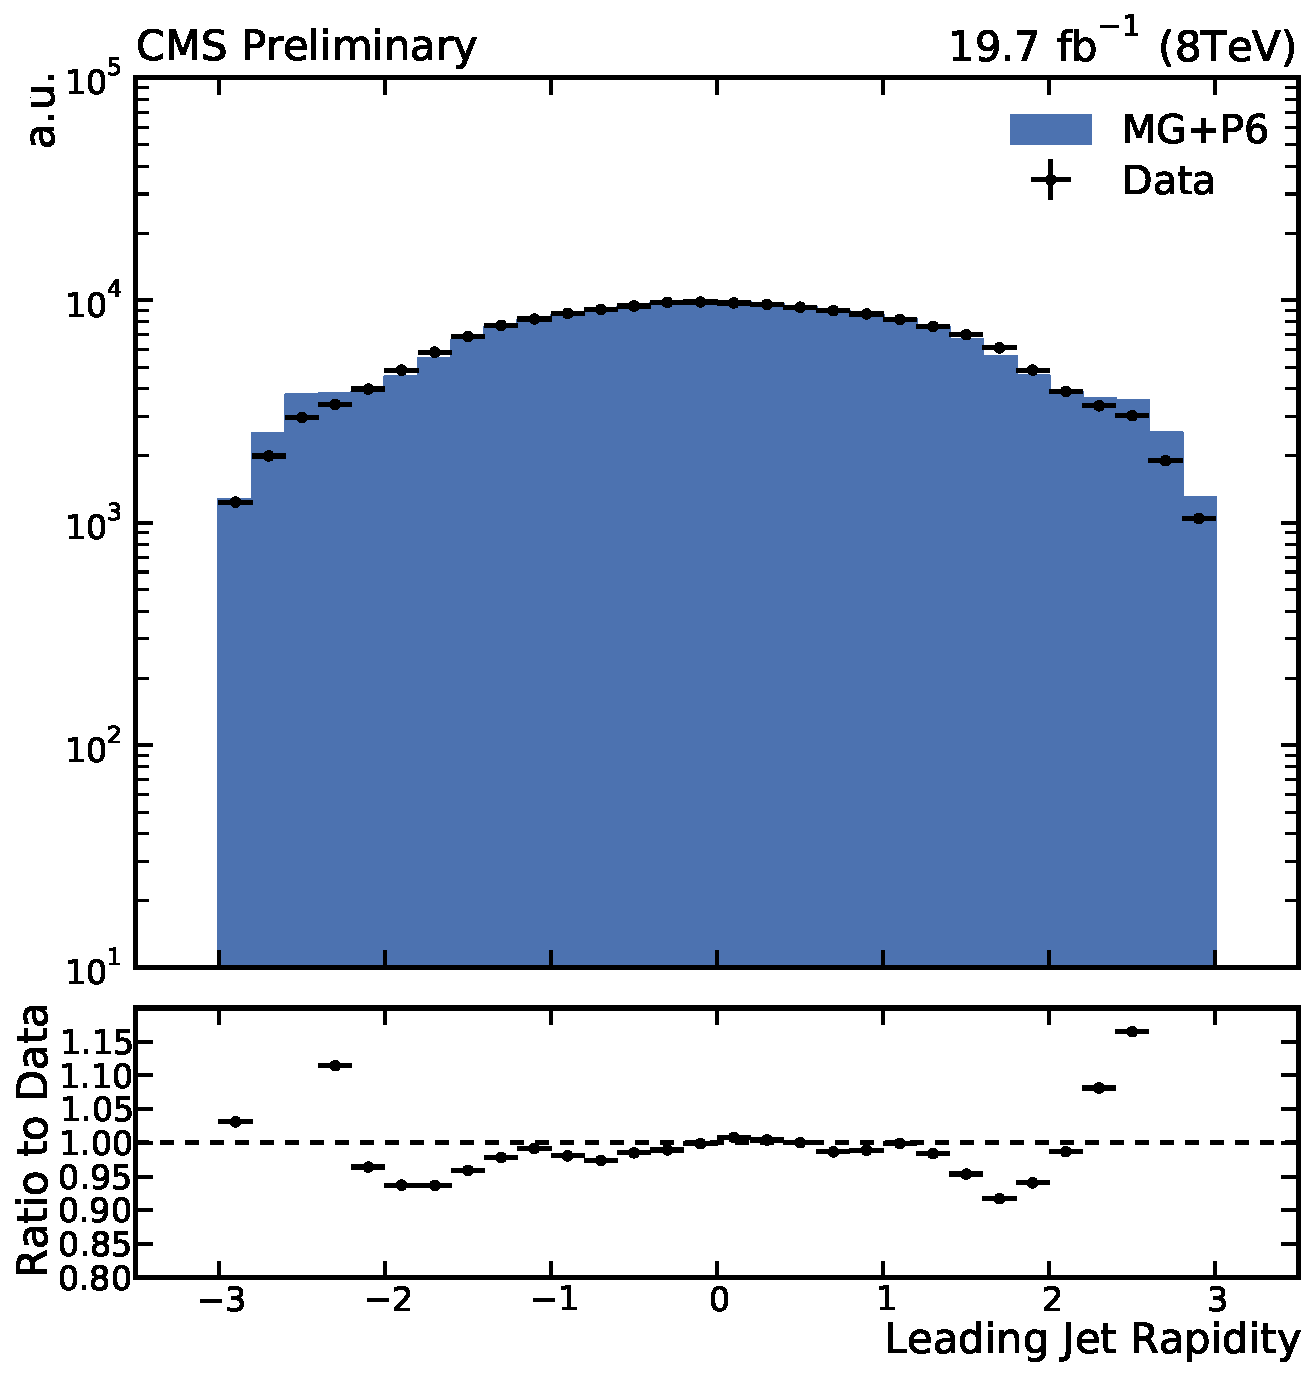
\includegraphics[width=0.45\textwidth]{figures/measurement/jet1rap_default.pdf}\hfill
    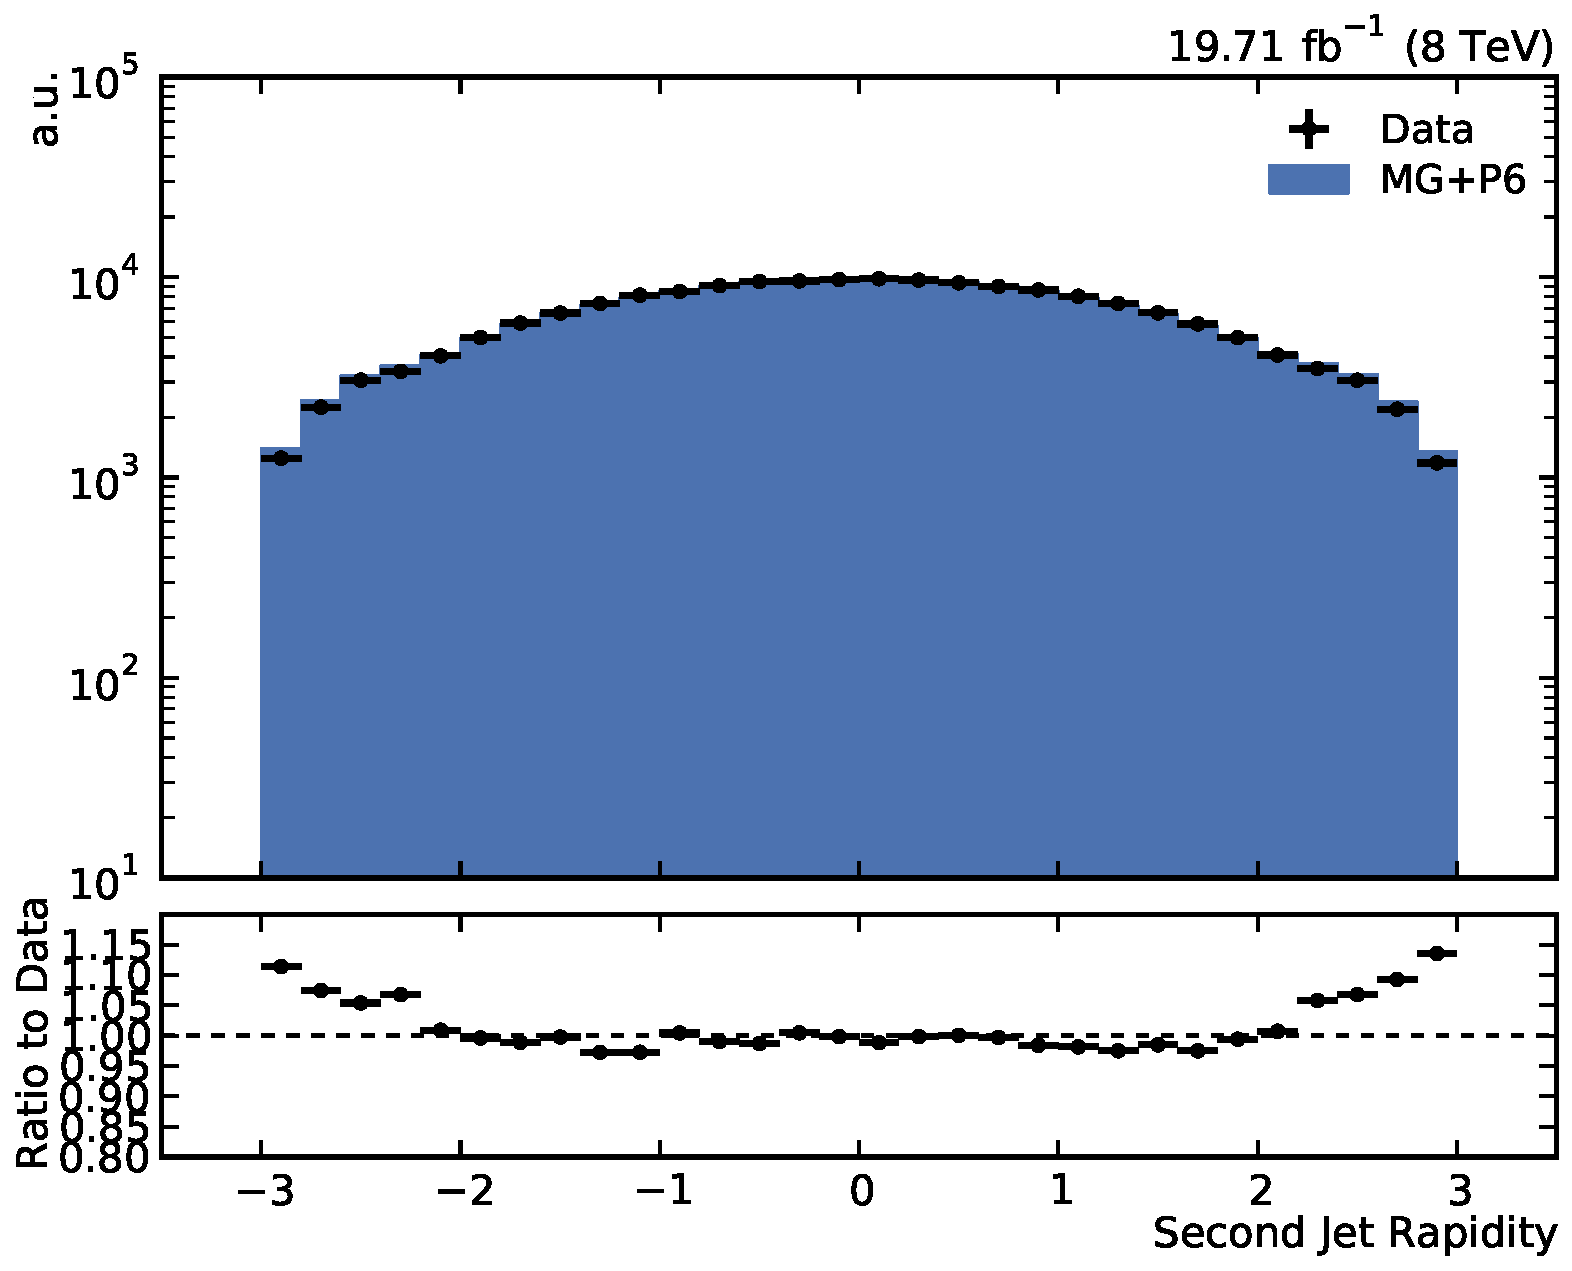
\includegraphics[width=0.45\textwidth]{figures/measurement/jet2rap_default.pdf}
    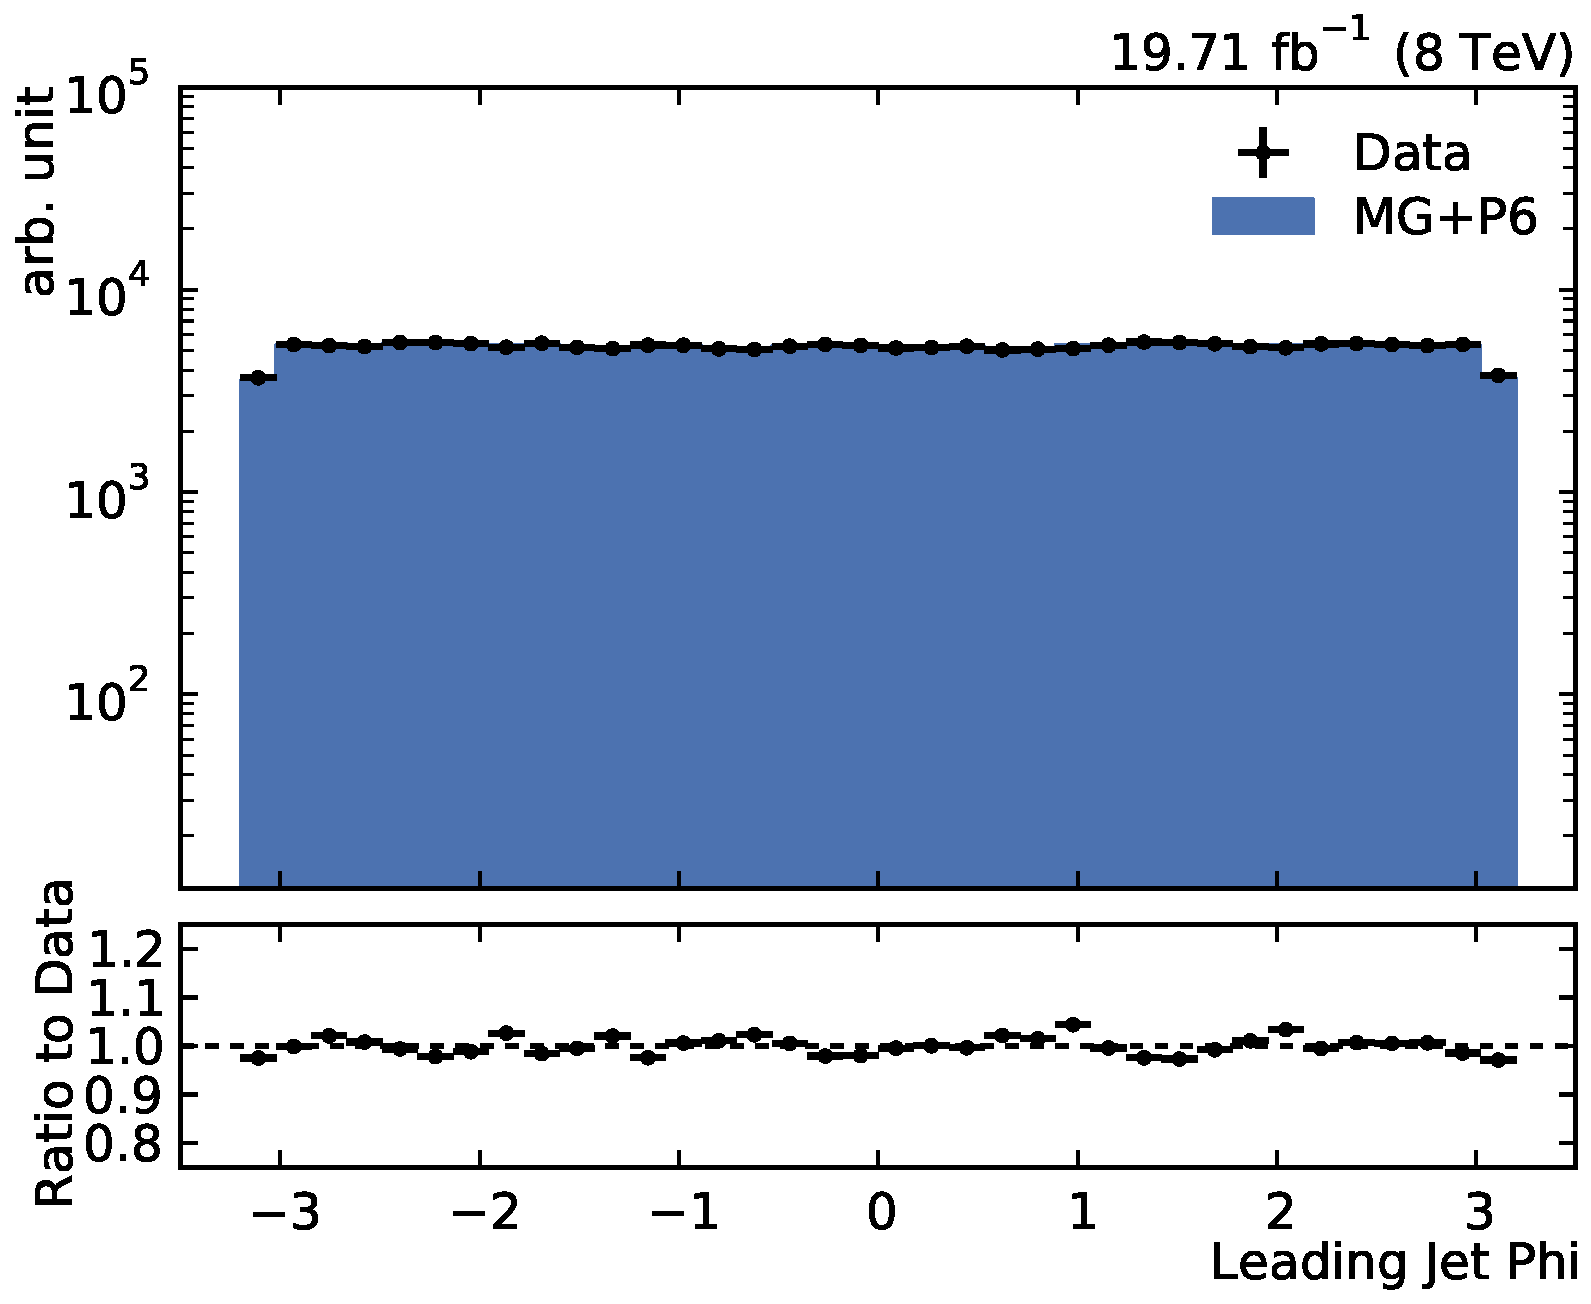
\includegraphics[width=0.45\textwidth]{figures/measurement/jet1phi_default.pdf}\hfill
    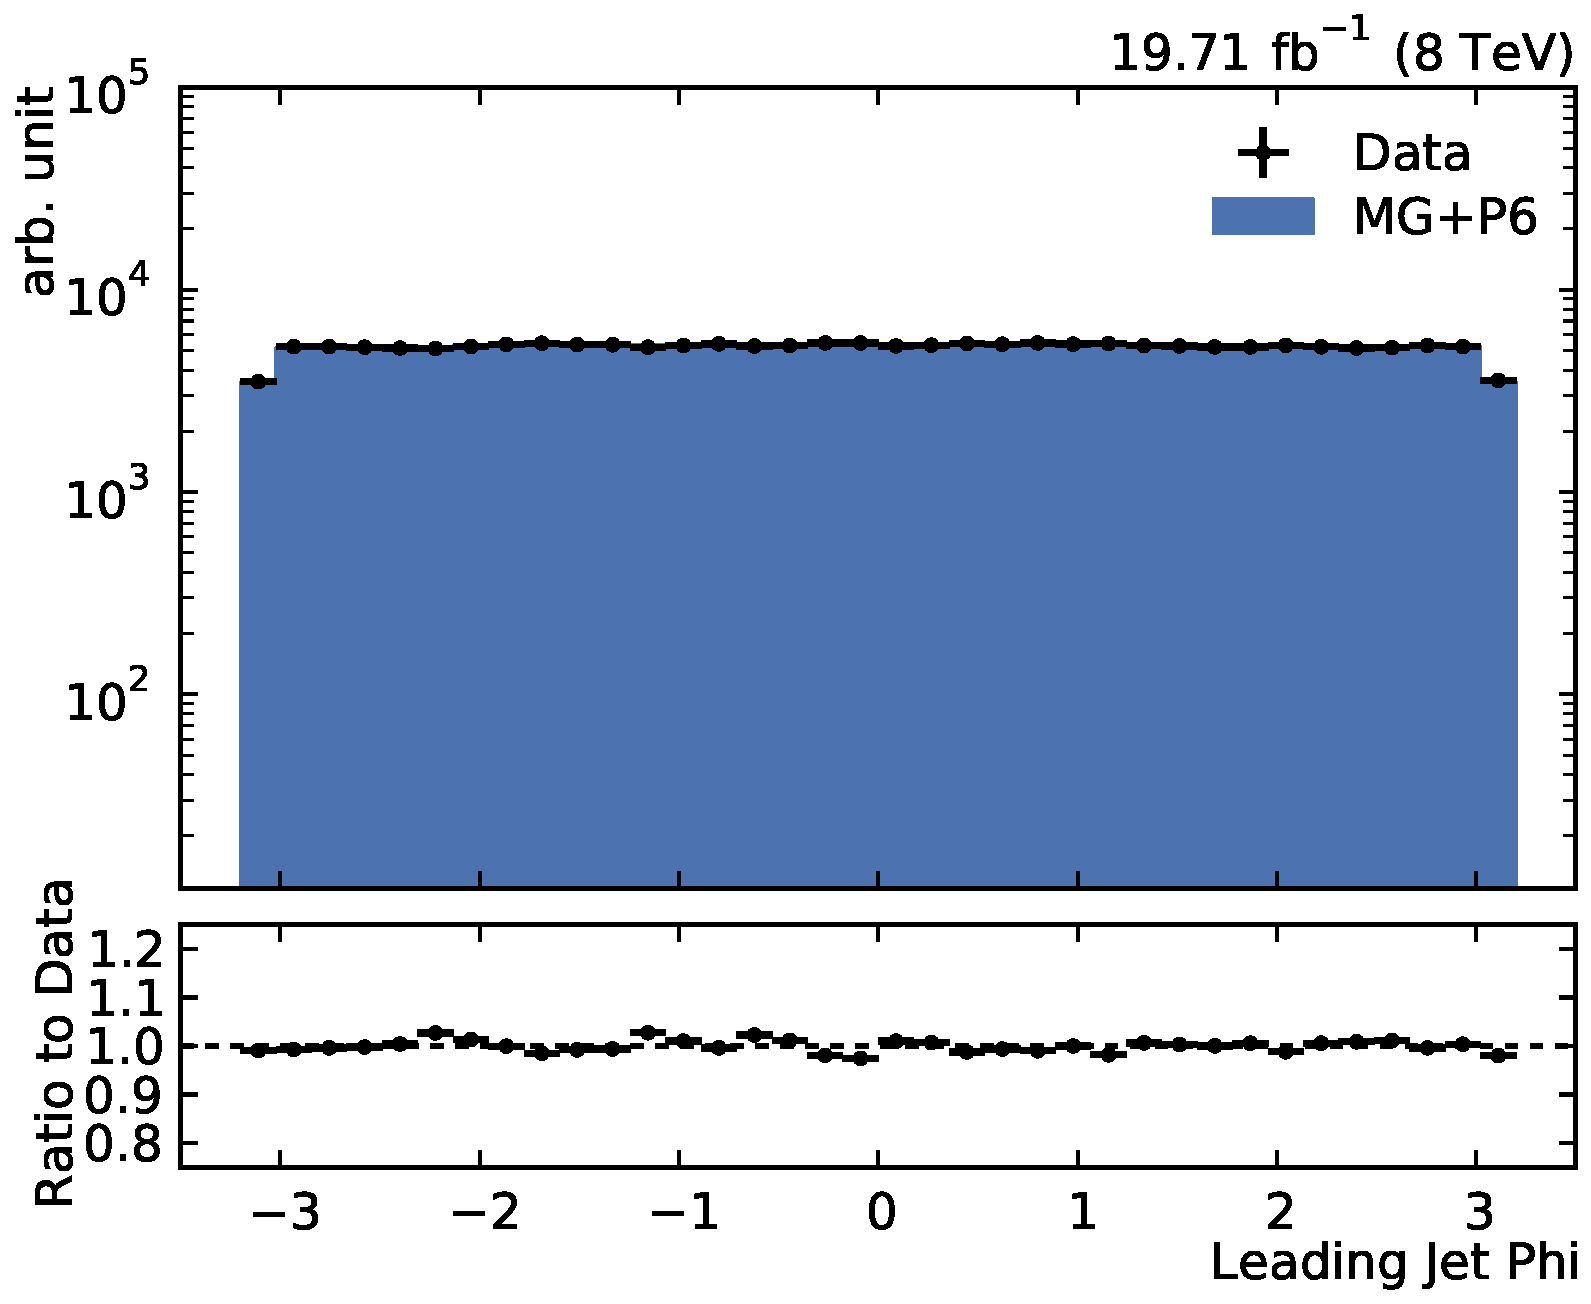
\includegraphics[width=0.45\textwidth]{figures/measurement/jet2phi_default.pdf}
    \caption{The plots show the basic kinematic quantities of the two leading jets in a selected event.
             The transvers momentum of the leading (left plot) and the second (right plots) jet is shown
         in the top row. The rapidity of the jets is shown in the middle row. The azimuthal angle of the
     leading jet and the second jet is shown on the bottom row.}
    \label{fig:controlplots:kinematic}
\end{figure}

\begin{figure}[htbp]
    \centering
    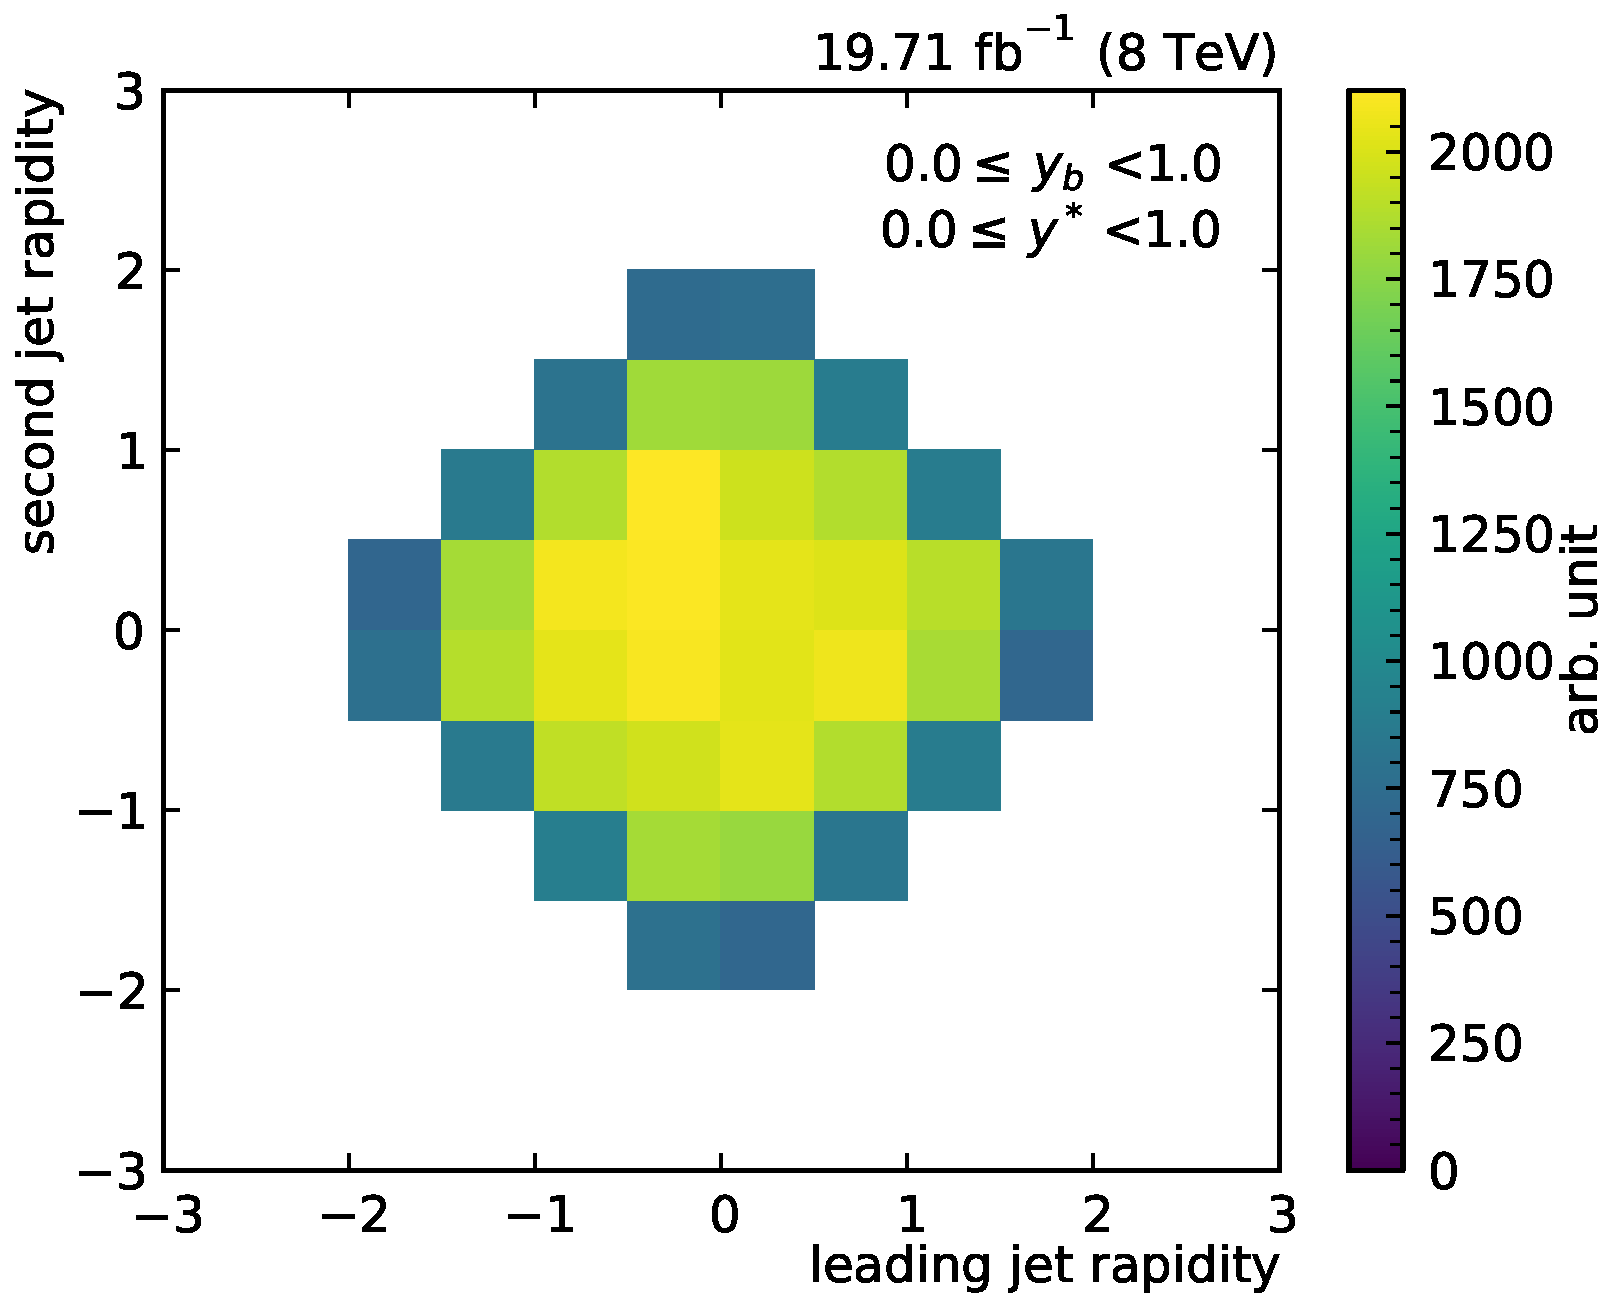
\includegraphics[width=0.45\textwidth]{figures/measurement/jet12_rapidity_yb0ys0.pdf}\hfill
    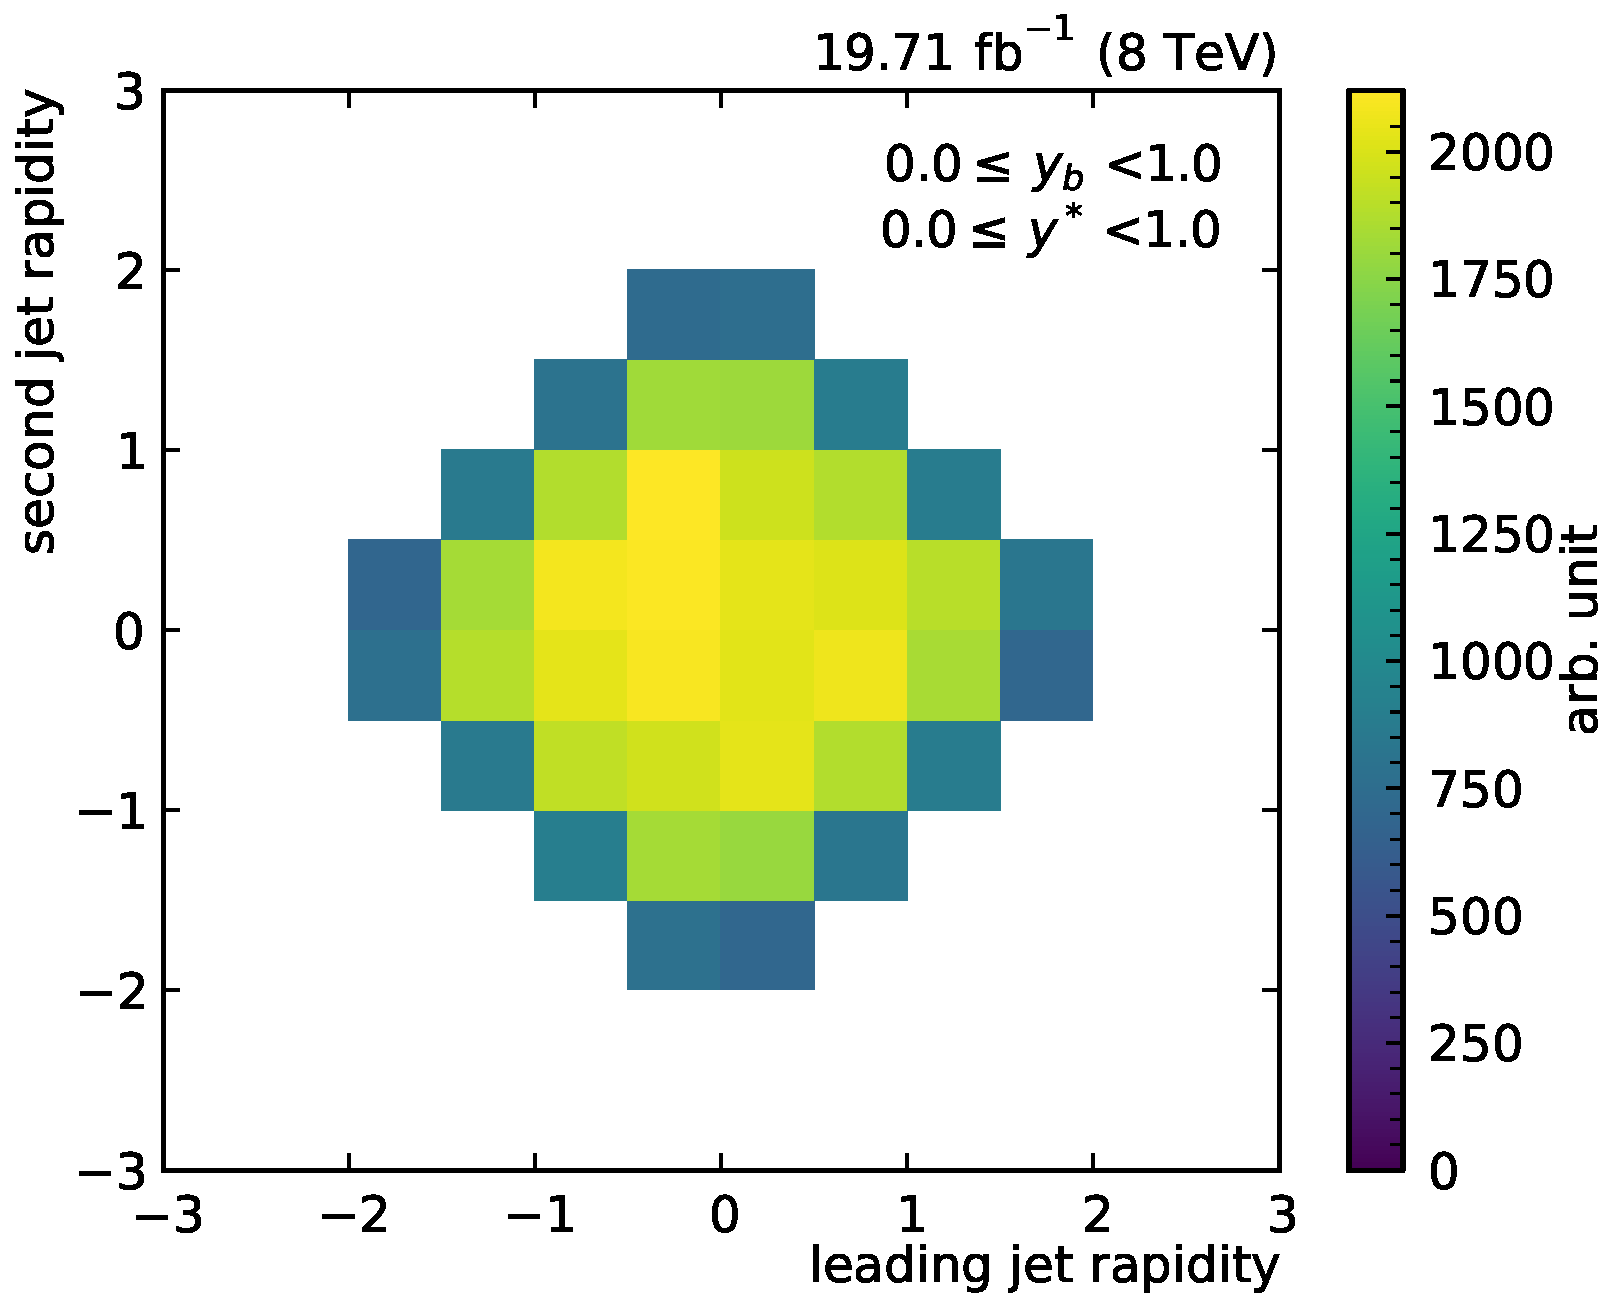
\includegraphics[width=0.45\textwidth]{figures/measurement/jet12_rapidity_yb0ys0.pdf}
    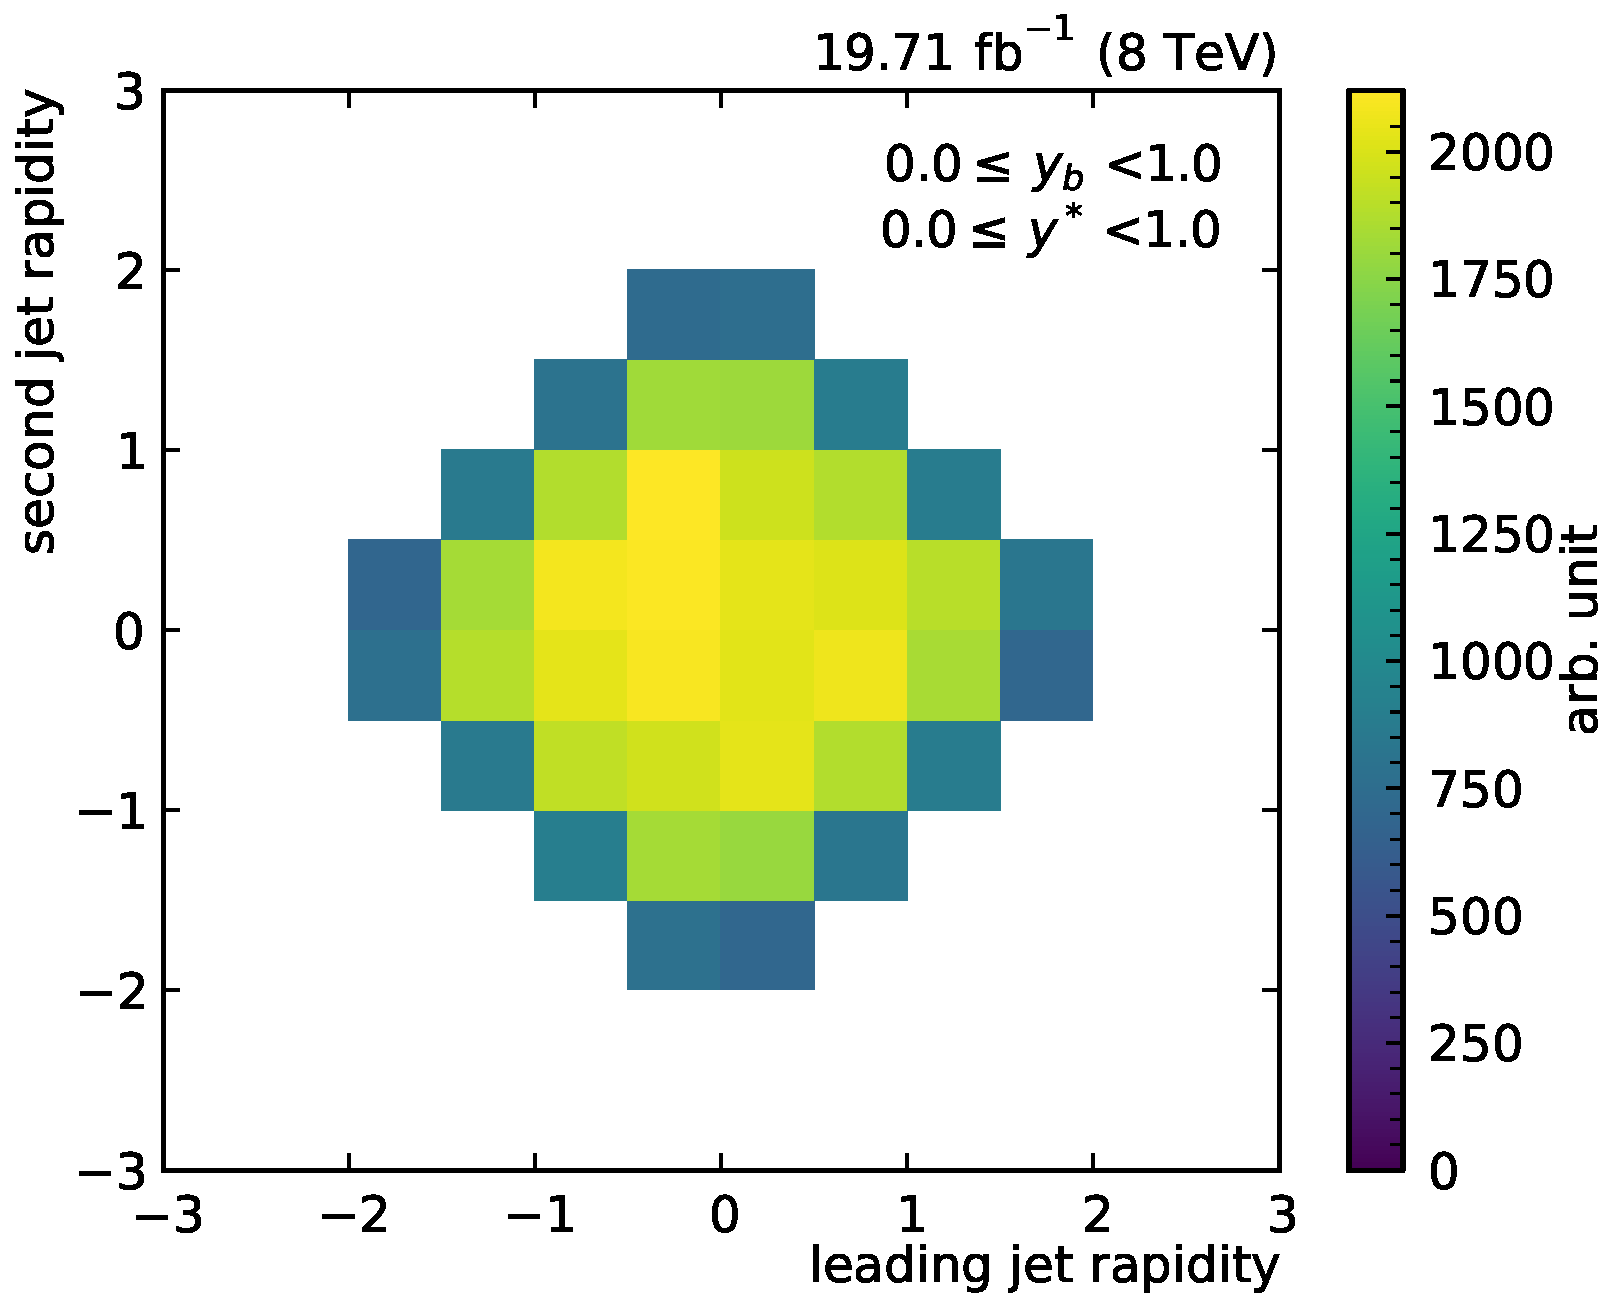
\includegraphics[width=0.45\textwidth]{figures/measurement/jet12_rapidity_yb0ys0.pdf}\hfill
    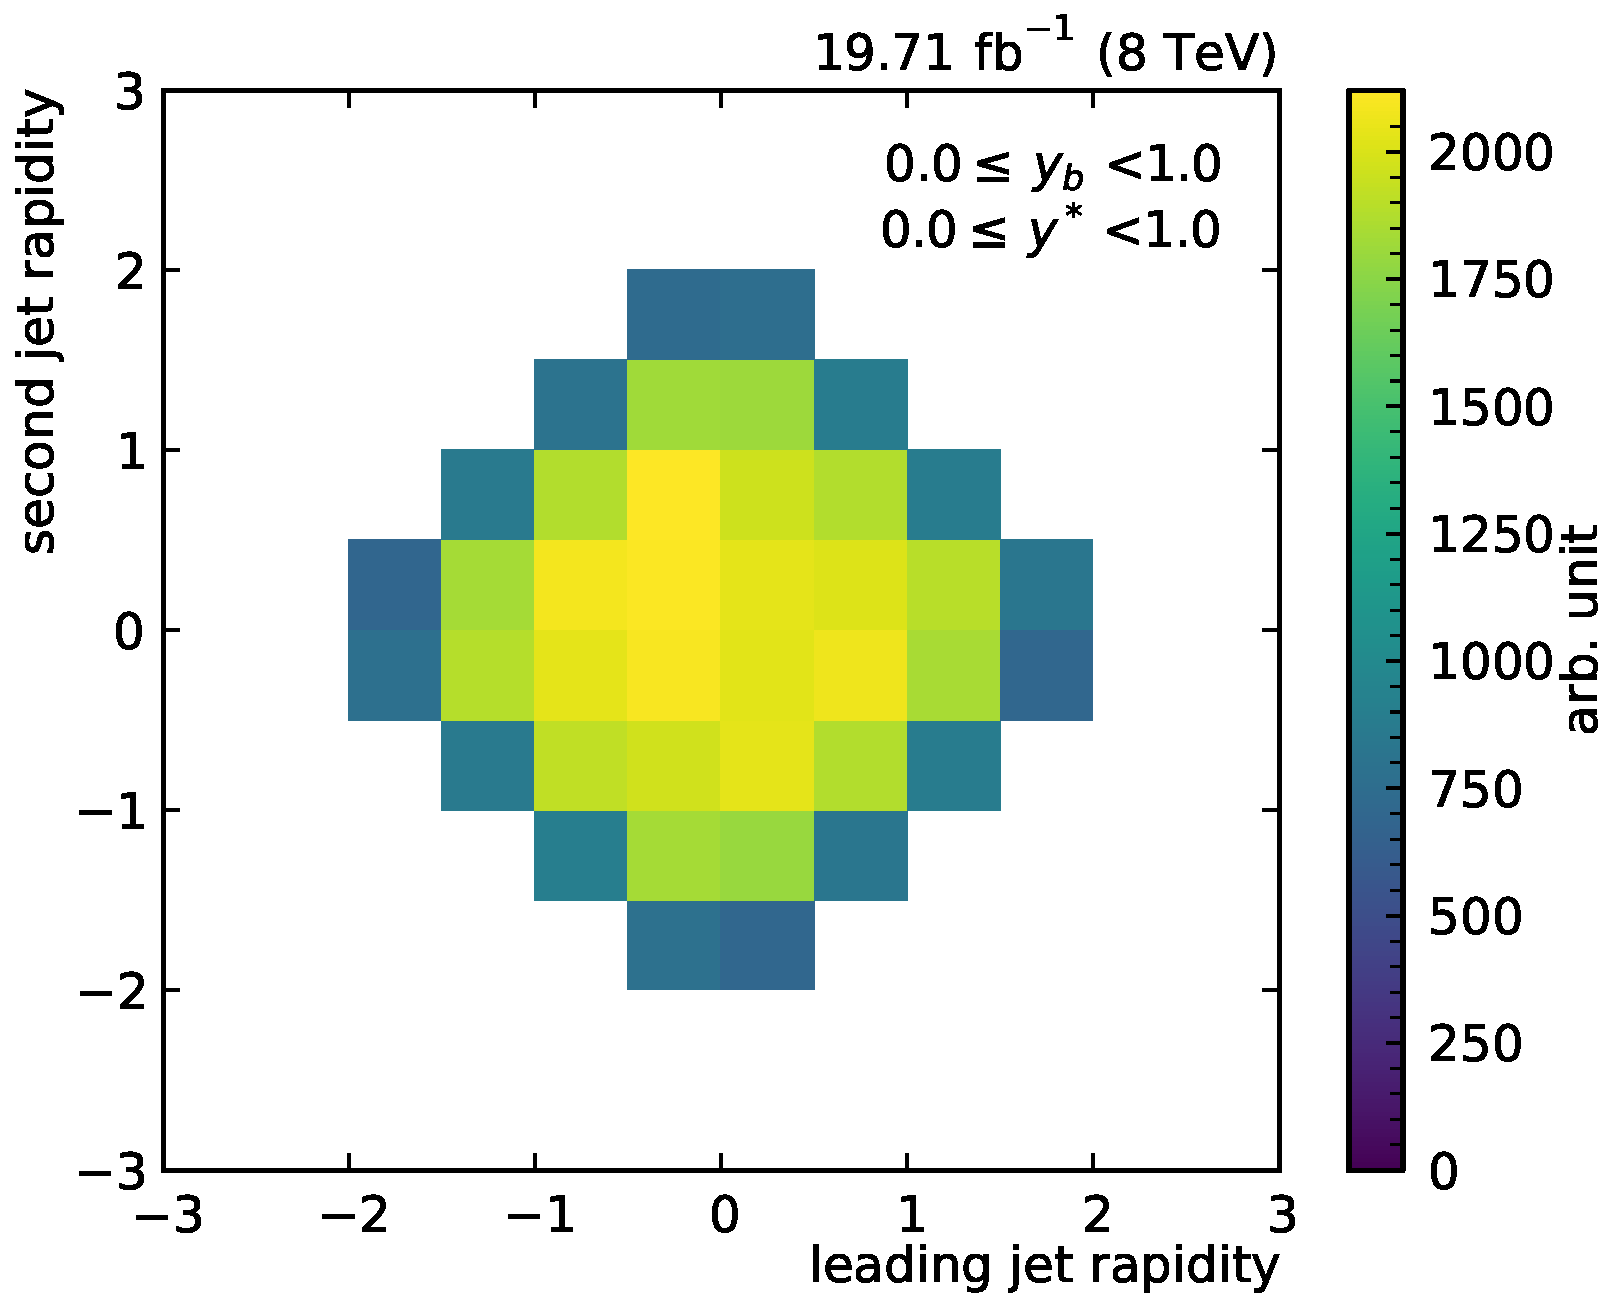
\includegraphics[width=0.45\textwidth]{figures/measurement/jet12_rapidity_yb0ys0.pdf}
    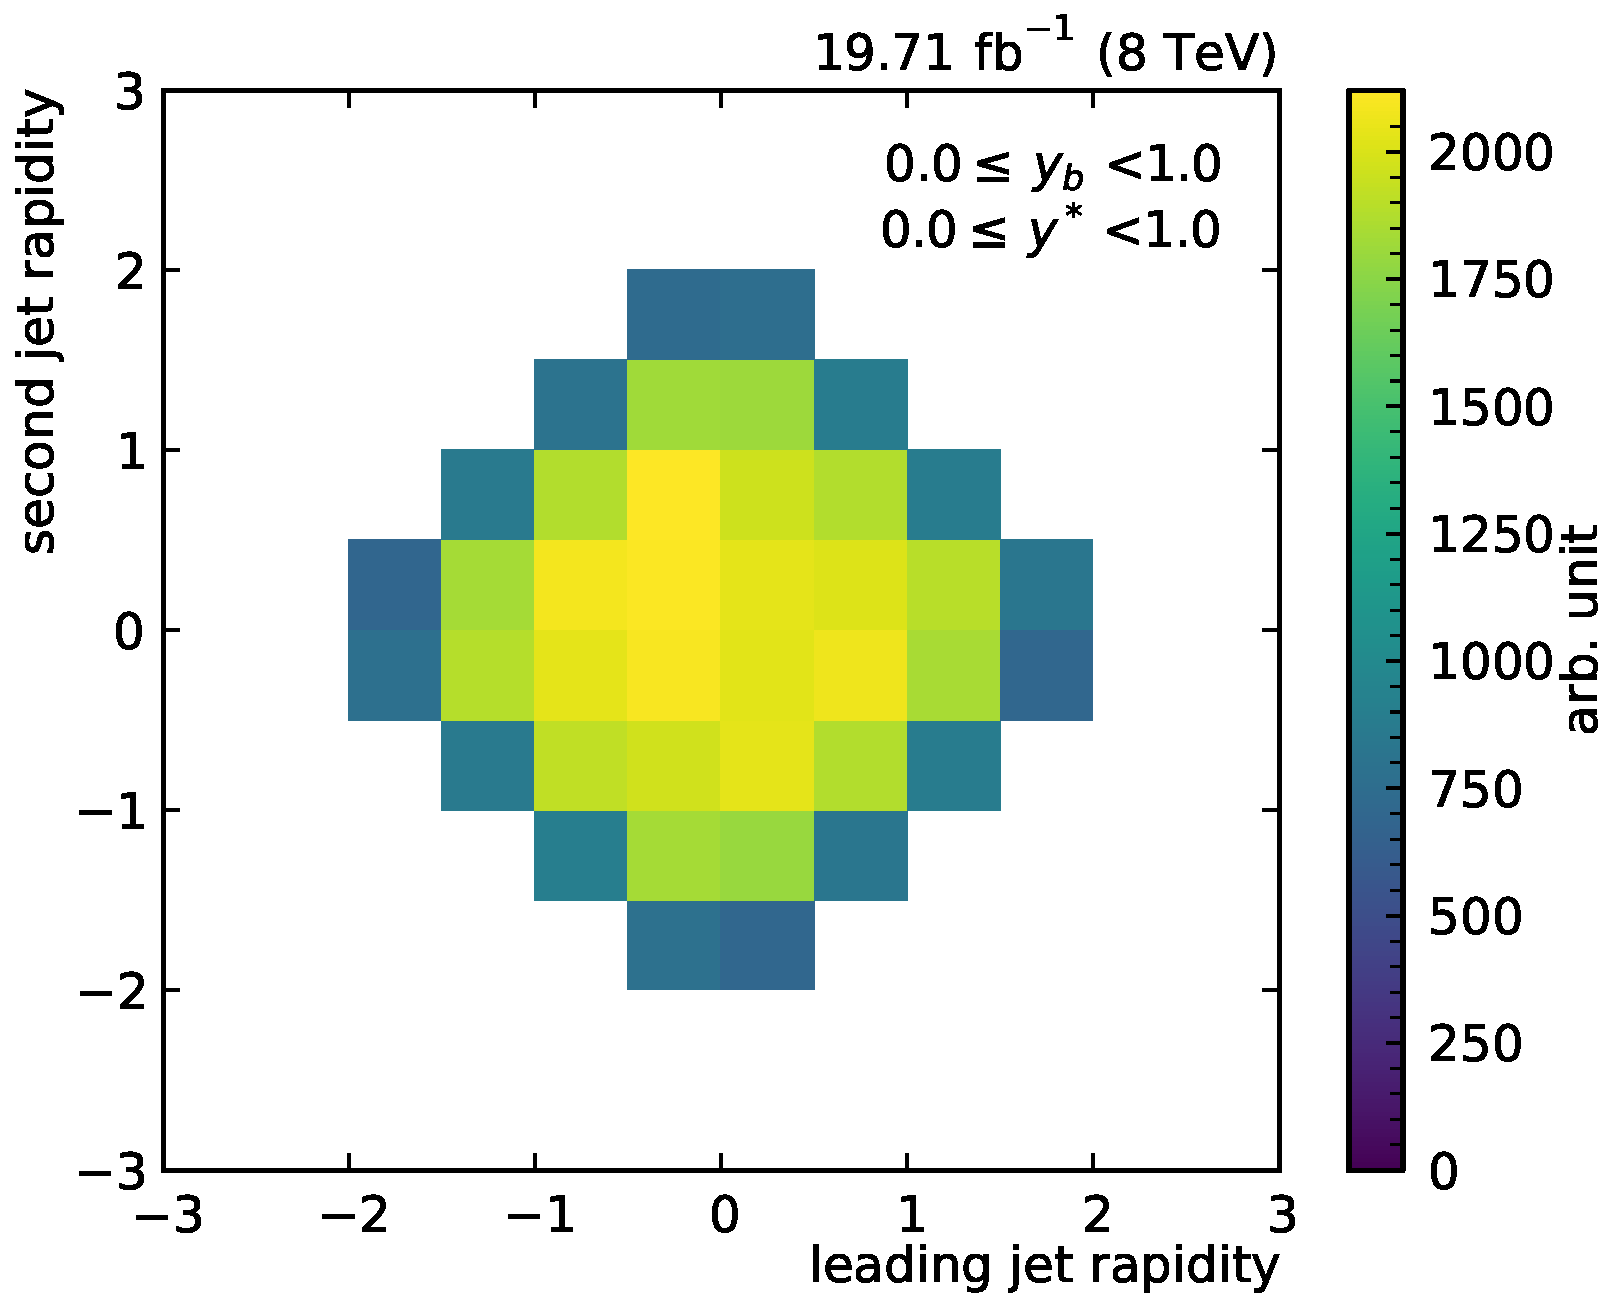
\includegraphics[width=0.45\textwidth]{figures/measurement/jet12_rapidity_yb0ys0.pdf}\hfill
    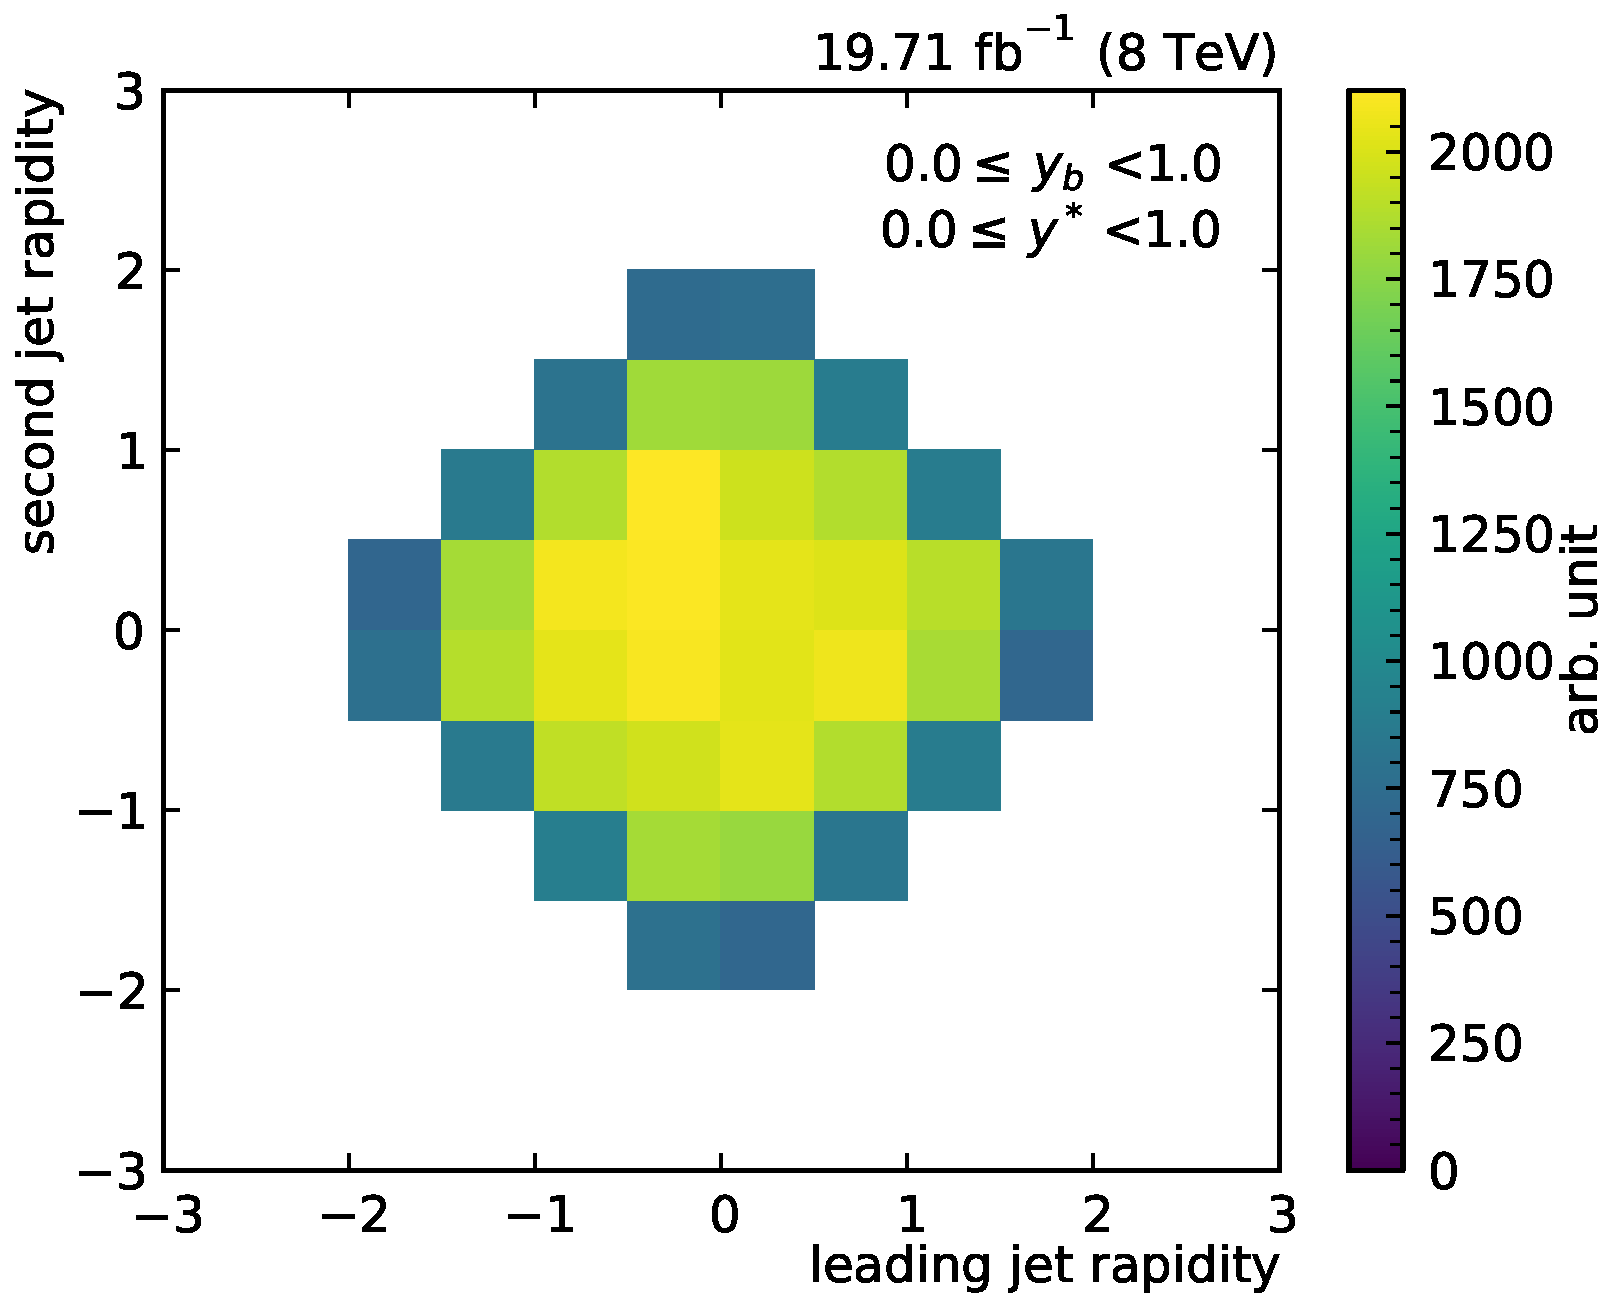
\includegraphics[width=0.45\textwidth]{figures/measurement/jet12_rapidity_yb0ys0.pdf}
    \caption{The plots show the basic kinematic quantities of the two leading jets in a selected event.
             The transvers momentum of the leading (left plot) and the second (right plots) jet is shown
         in the top row. The rapidity of the jets is shown in the middle row. The azimuthal angle of the
     leading jet and the second jet is shown on the bottom row.}
    \label{fig:controlplots:rapidity}
\end{figure}


\subsection{Cross section Comparison}

The Monte-Carlo simulation is used to compare the prediction including the detector simulation
to the measured data distribution which is smeared due to the finite detector resolution. Figure~\ref{fig:ratio_recotodata}
show the prediction of the MG+P6 and the P8 simulations as a ratio to the measured data spectrum.
While the agreement in the inner detector region is fine, the shape and especially the normalization
of the MC prediction cannot describe the data. Additionally the fixed order prediction of NLOJET++
is shown. This prediction is on parton level and is not corrected for non-perturbative effects. Still
it describes best the data apart from the known effects due to NP and detector resolution effects.

\begin{figure}[htbp]
    \centering
    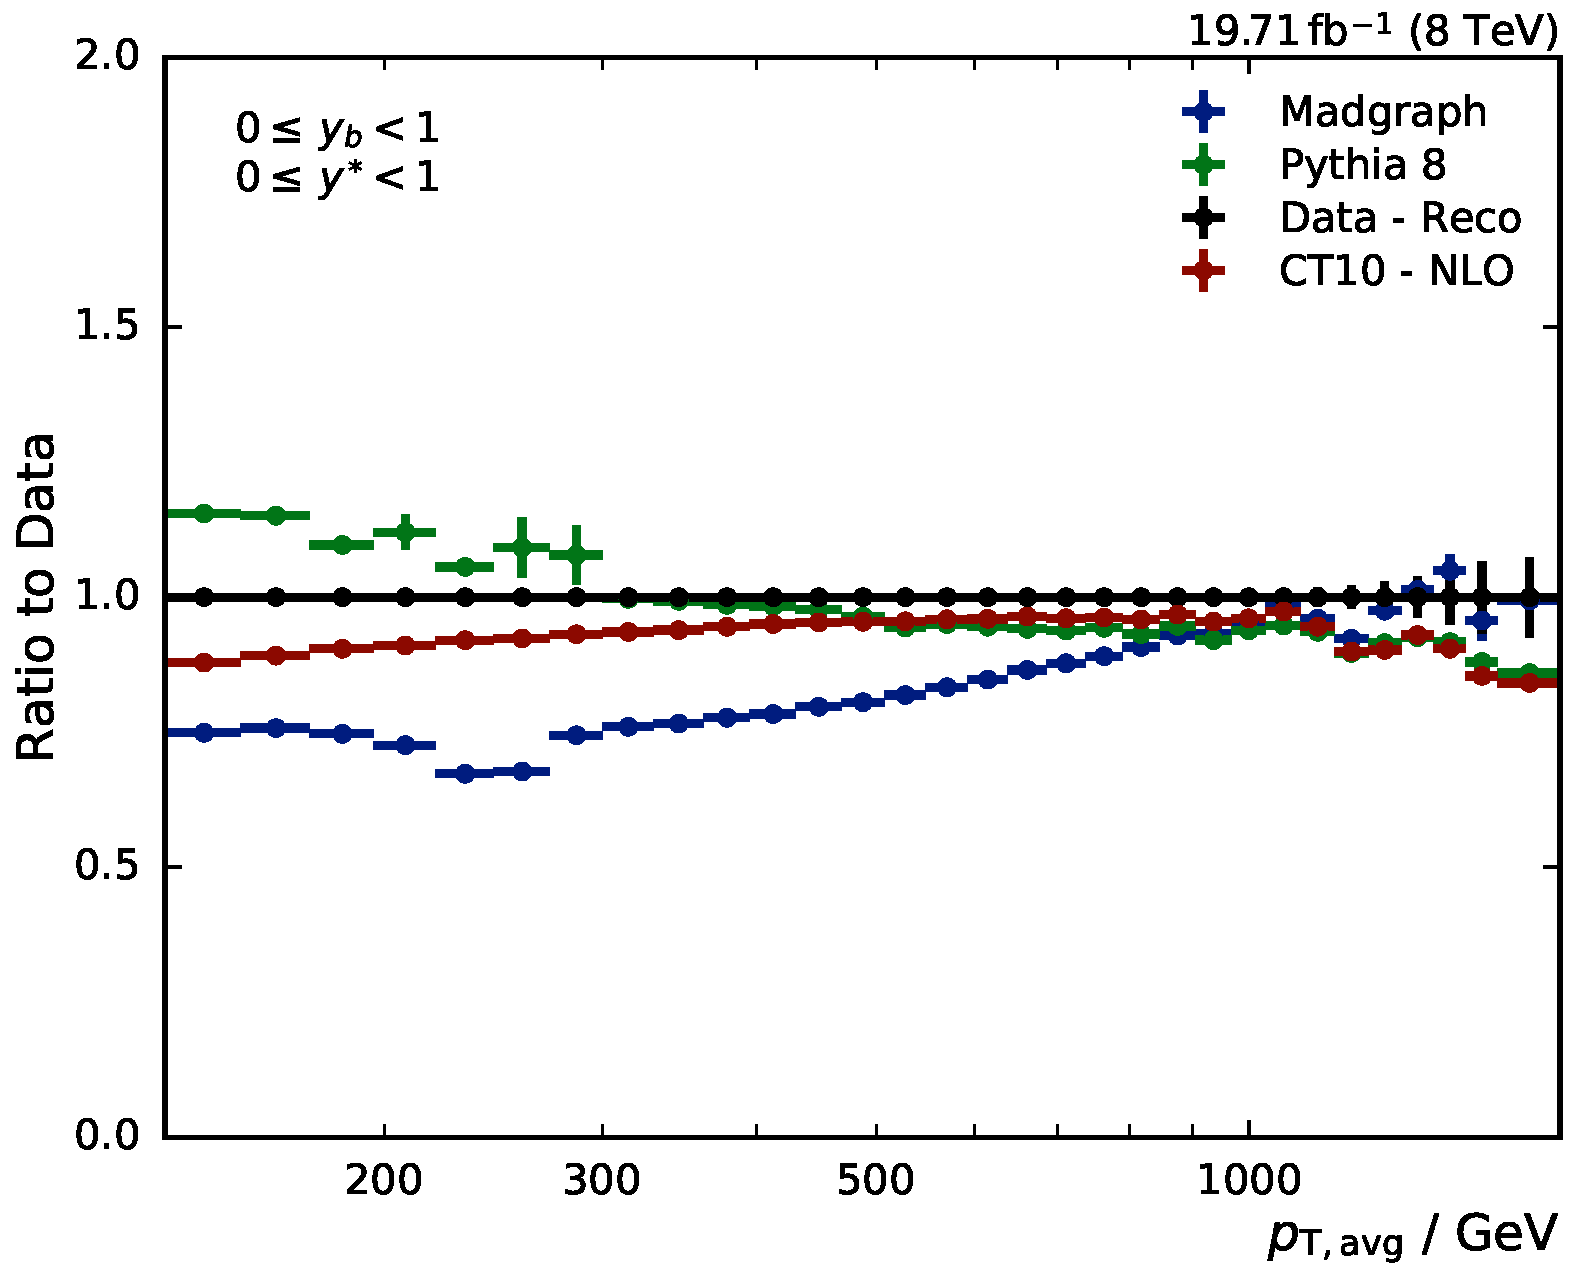
\includegraphics[width=0.45\textwidth]{figures/measurement/ratio_reco_to_data_yb0ys0.pdf}\hfill
    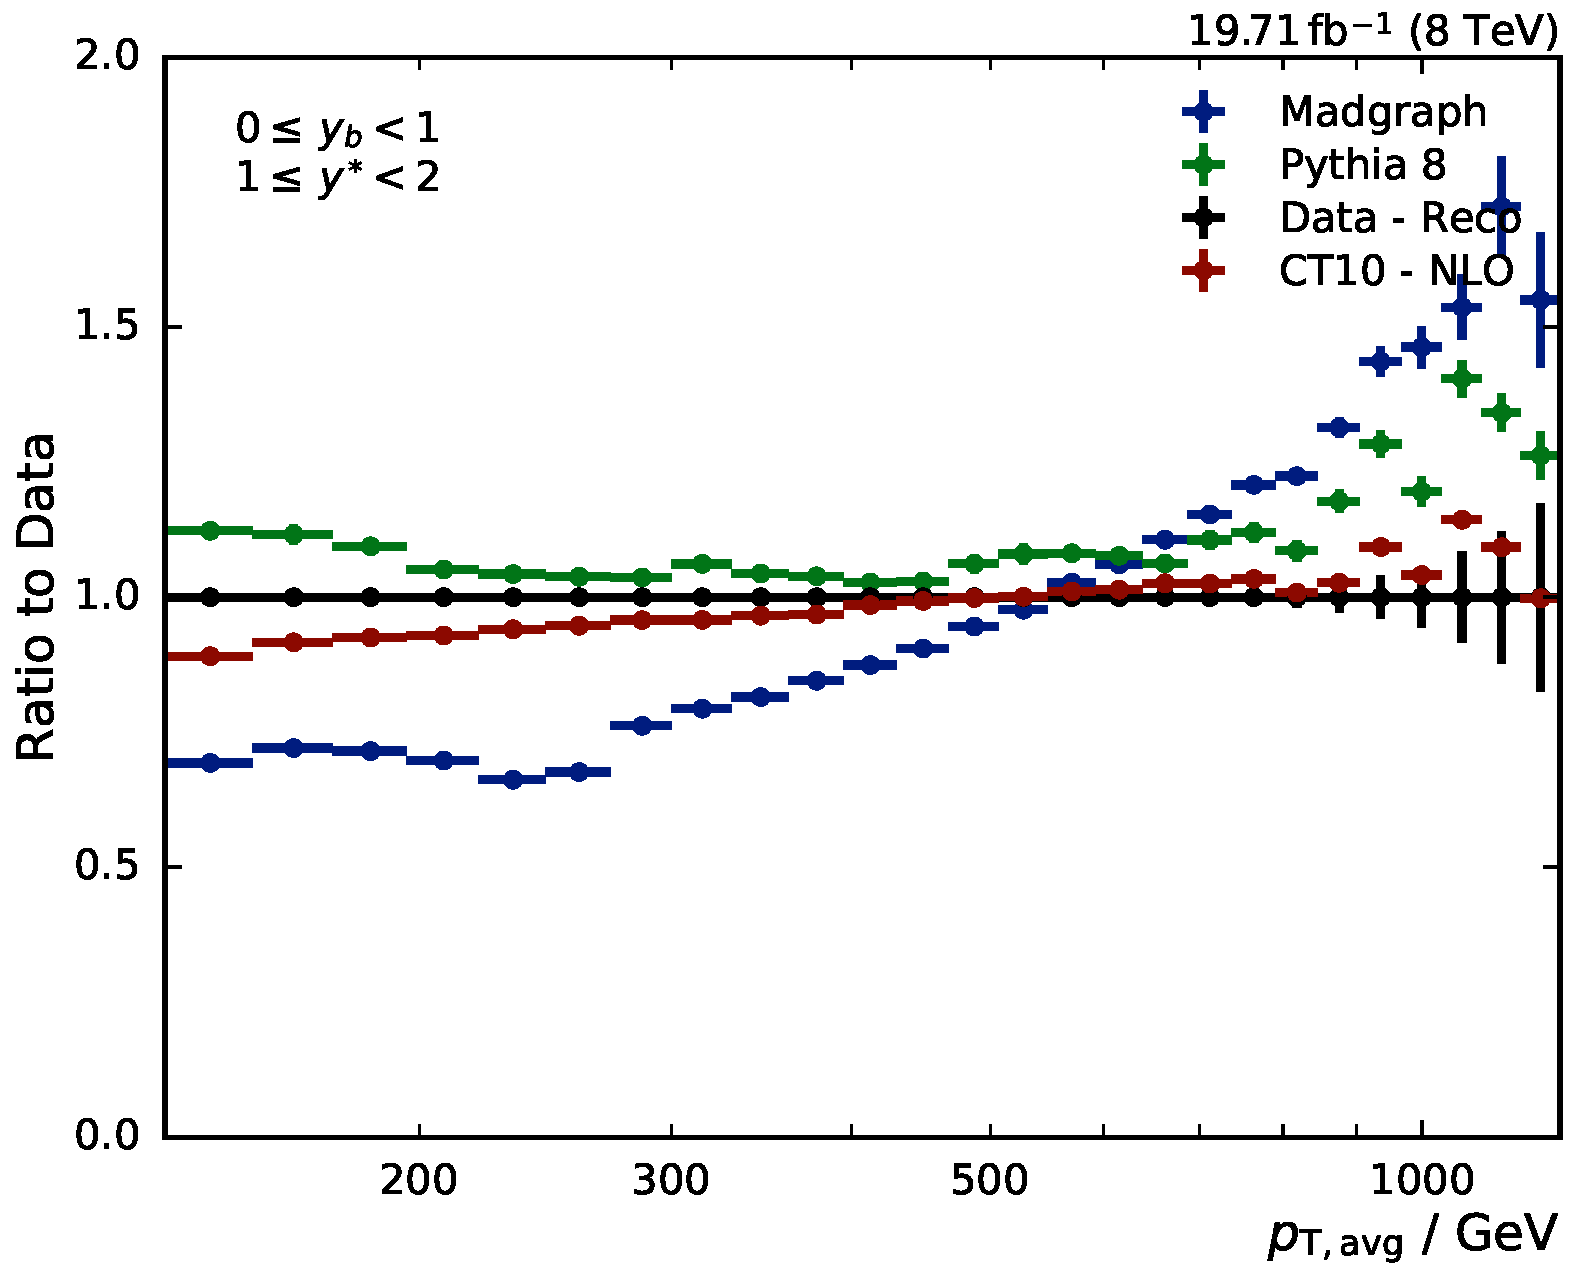
\includegraphics[width=0.45\textwidth]{figures/measurement/ratio_reco_to_data_yb0ys1.pdf}
    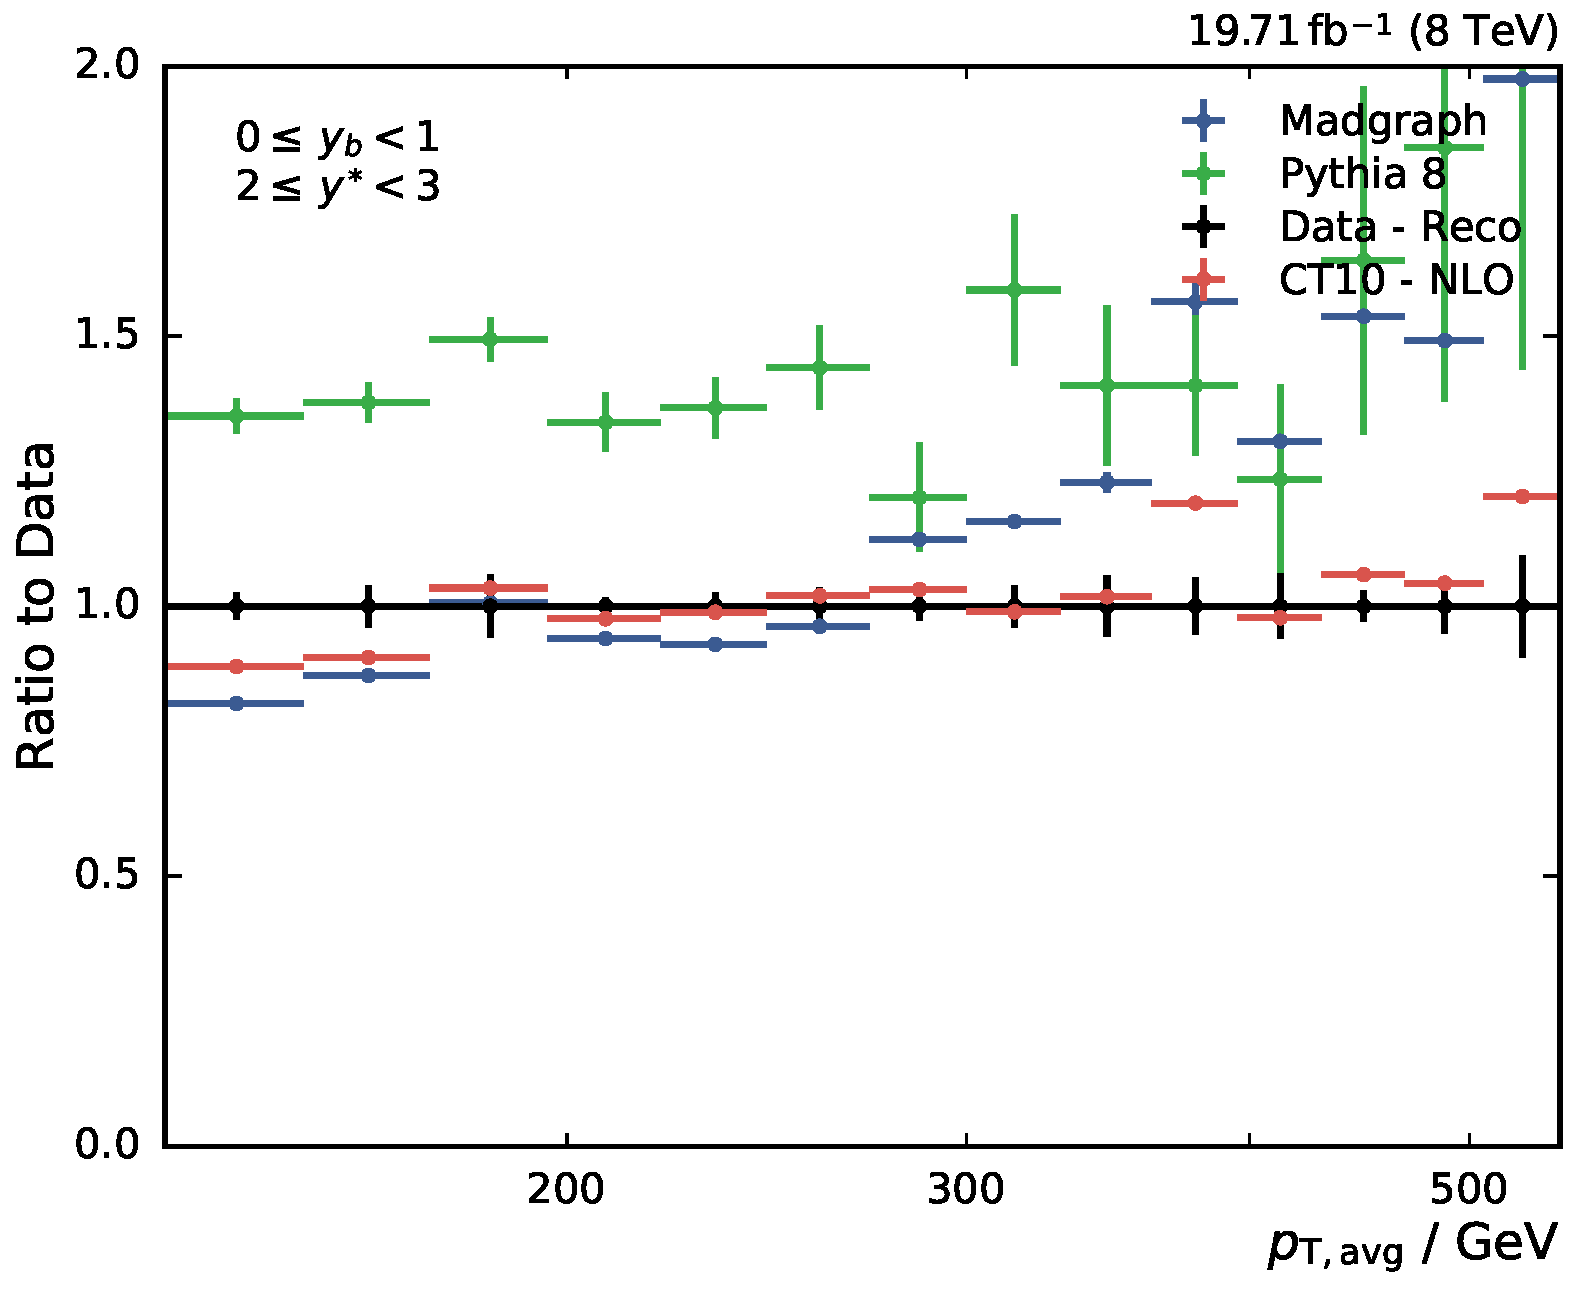
\includegraphics[width=0.45\textwidth]{figures/measurement/ratio_reco_to_data_yb0ys2.pdf}\hfill
    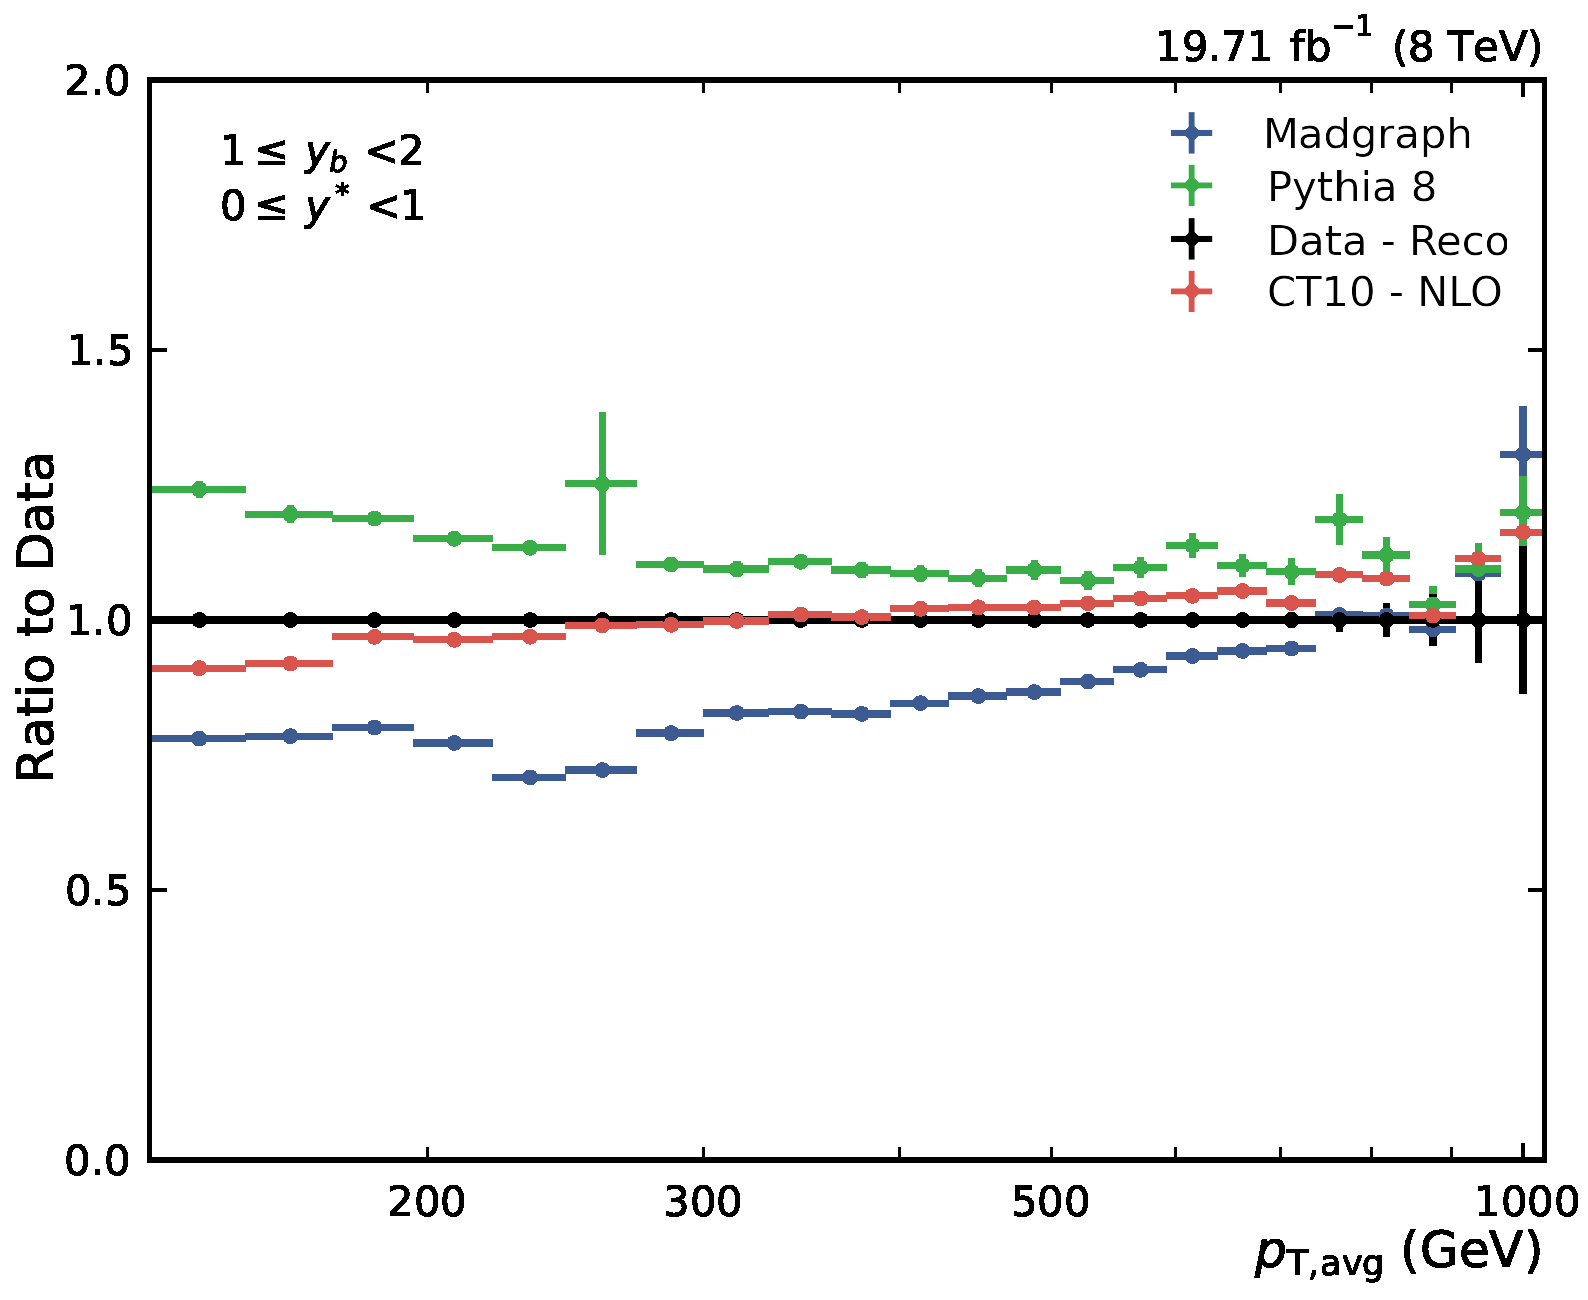
\includegraphics[width=0.45\textwidth]{figures/measurement/ratio_reco_to_data_yb1ys0.pdf}
    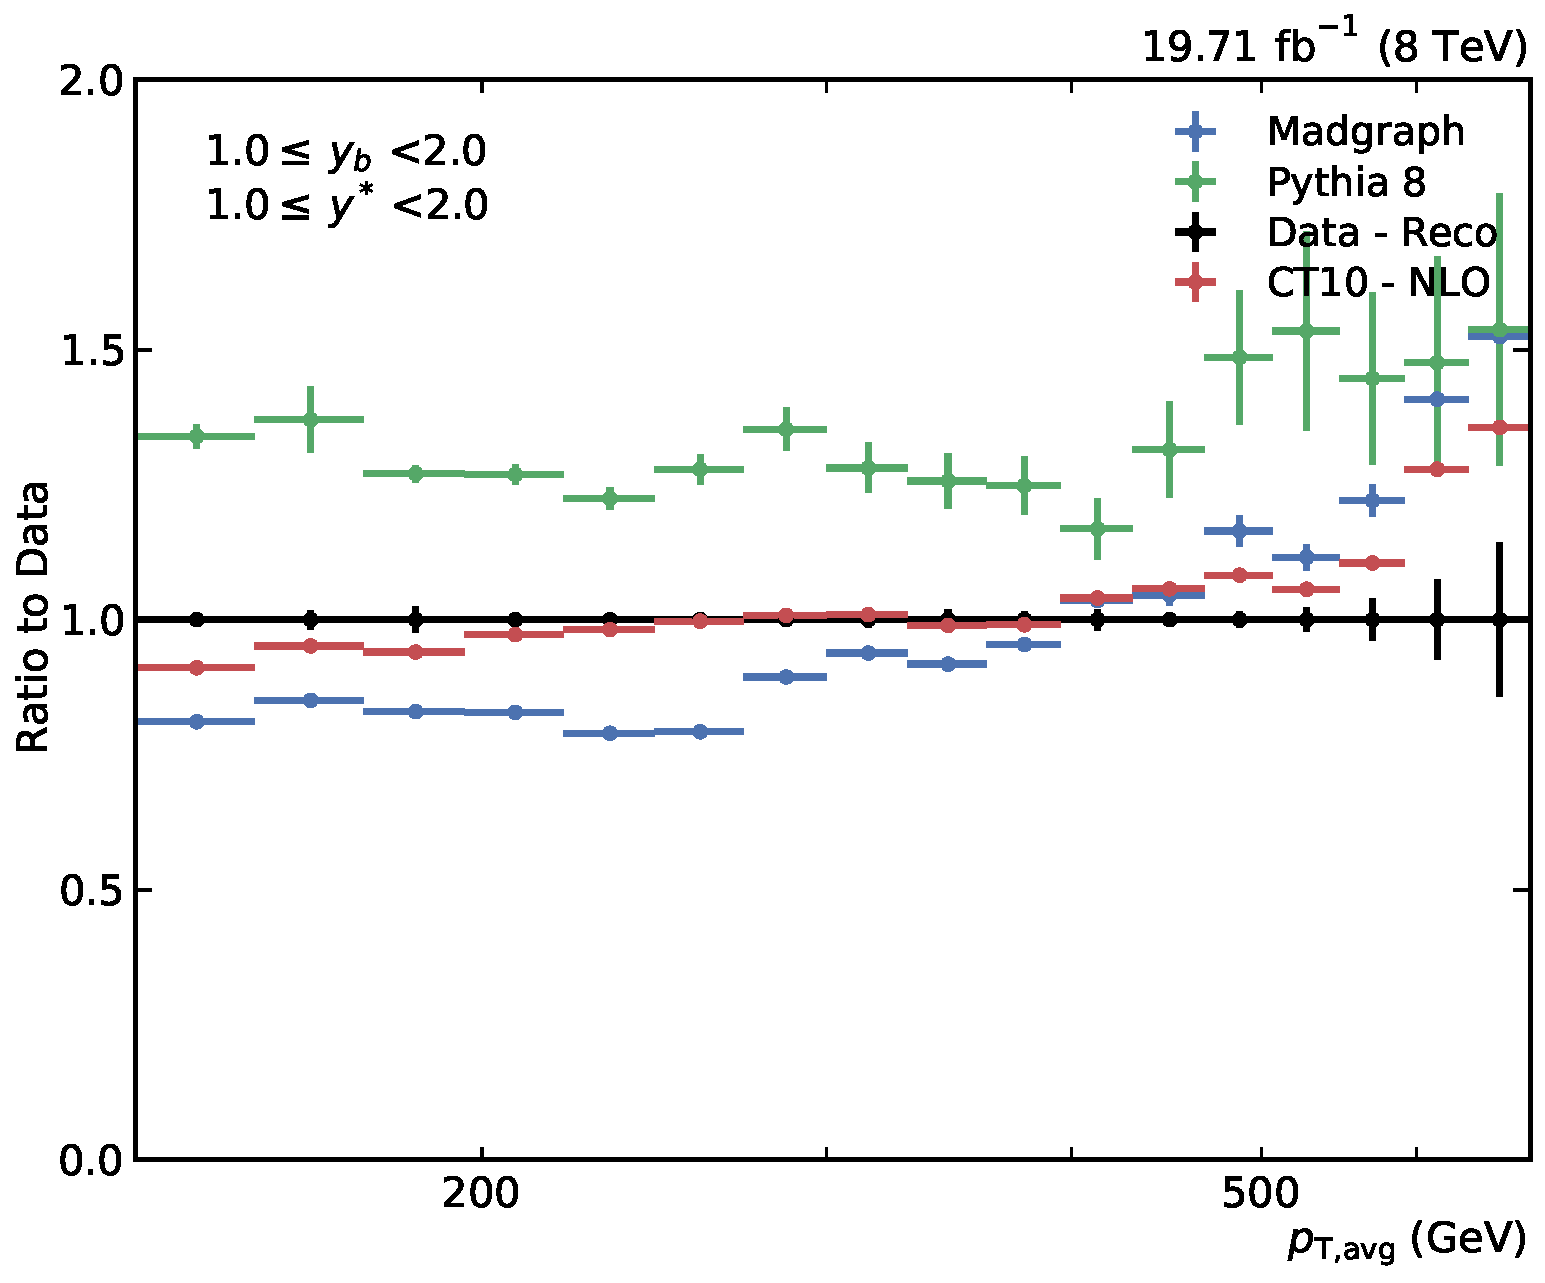
\includegraphics[width=0.45\textwidth]{figures/measurement/ratio_reco_to_data_yb1ys1.pdf}\hfill
    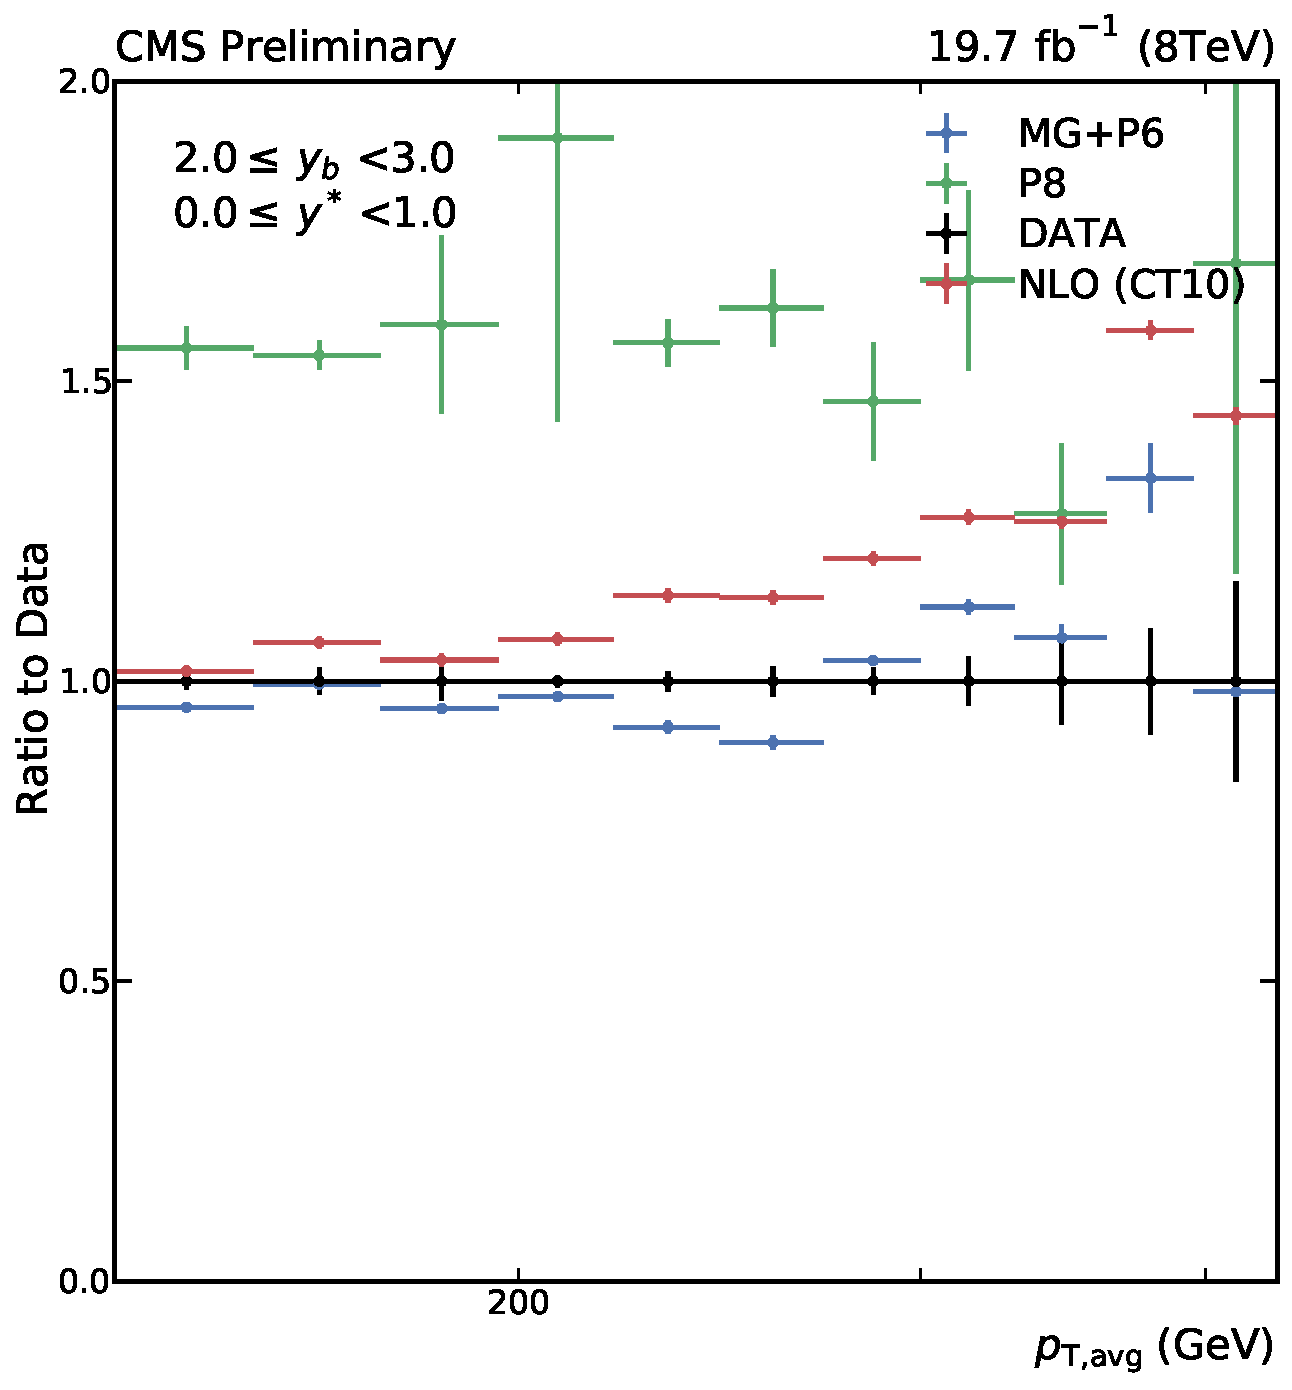
\includegraphics[width=0.45\textwidth]{figures/measurement/ratio_reco_to_data_yb2ys0.pdf}
    \caption{Comparison of the measurement and the predictions using P8 and MG+P6. The data distributions are normalized
    to the integrated luminosity, the simulated events to the number of generated events and the cross section. The ratio of the simulated
    events to the data points is shown.}
    \label{fig:ratio_recotodata}
\end{figure}


\todo{figure with jet rapidities?}

\section{Dijet Transverse Momentum  Resolution}
\label{sec:resolution}

The true transverse momentum of the jets is smeared through the finite
resolution of the CMS detector. To measure the resolution of the \ptavg
observable, the truth information of Monte-Carlo events propagated through the
detector is used. The jets are clustered from stable generator particles as well
as from particle flow candidates reconstructed from the simulated detector
output. When studying the resolution, only events in which the leading two
generator jets are well matched to the reconstructed jets are used. The distance
$\Delta R$ in the $\eta$-$\phi$ plane is calculated as

\begin{equation}
\Delta R = \sqrt{\Delta \eta^2 + \Delta \phi^2}
\end{equation}
and needs to satisfy $\Delta R < 0.3$.

Measurements of the JERC working group at CMS show that the jet energy
resolution in data is actually worse than in simulation and the reconstructed
jet transverse momentum needs to be smeared additonally to match the resolution
in data. Table~\ref{tab:res_smearing} shows the smearing factors which need to
be applied on the transverse momentum of simulated reconstructed jets. The
smearing factors are derived separately for each region of the detector geometry.

\begin{table}[htbp]
\setlength\tabcolsep{4.5pt} 
    \centering
    \begin{tabular}{lccccccr}
    \toprule
    & & \multicolumn{6}{c}{$|\eta|$}\\\cmidrule{2-8}
               & $0.0$ -- $0.5$ & $0.5$ -- $1.1$ & $1.1$ -- $1.7$ & $1.7$ --
               $2.3$ & $2.3$ -- $2.8$ & $2.8$ -- $3.2$ & $3.2$ -- $5.0$\\
               $c_\text{res}$ &  &  &  & & & & \\\cmidrule{1-1}
    central    & 1.079                   & 1.099                   & 1.121    & 1.208                   & 1.254                   & 1.395    & 1.056\\
    down       & 1.053                   & 1.071                   & 1.092    & 1.162                   & 1.192                   & 1.332 & 0.865\\
    up         & 1.105                   & 1.127                   & 1.150 & 1.254                   & 1.316                   & 1.458 & 1.247\\
    \bottomrule
    \end{tabular}
    \caption{Since the resolution in data is significantly
             worse than in MC, the reco jet \pt was smeared using factors obtained from the
             JER twiki~\cite{JERC:Resolution}.}
    \label{tab:res_smearing}
\end{table}

Each reconstructed jet which is matched to a generated jet is smeared  using the formula
\begin{equation}
\ptreco = \max \left( 0, \ptgen + c(\eta) \cdot (\ptreco - \ptgen) \right)
\end{equation}

After applying the mentioned correction factor, the average dijet
transverse momentum is calculated both using the generator particle jets and
the particle flow jets on detector level. The response $R$ is calculated as

\begin{equation}
    R = \frac{\ptavg^{\text{reco}}}{\ptavg^{\text{gen}}}
\end{equation}

Since the response is dependent on the detector region as well as the transverse
momentum of the jets, the dijet average transverse momentum resolution is
calculated as a function of \ptavggen for each measurement bin in the phase
space variables \ystar and \yboost. Figure~\ref{fig:gen_vs_reco_over_gen} shows the
two-dimensional distributions for each bin.

\begin{figure}[htbp]
    \centering
    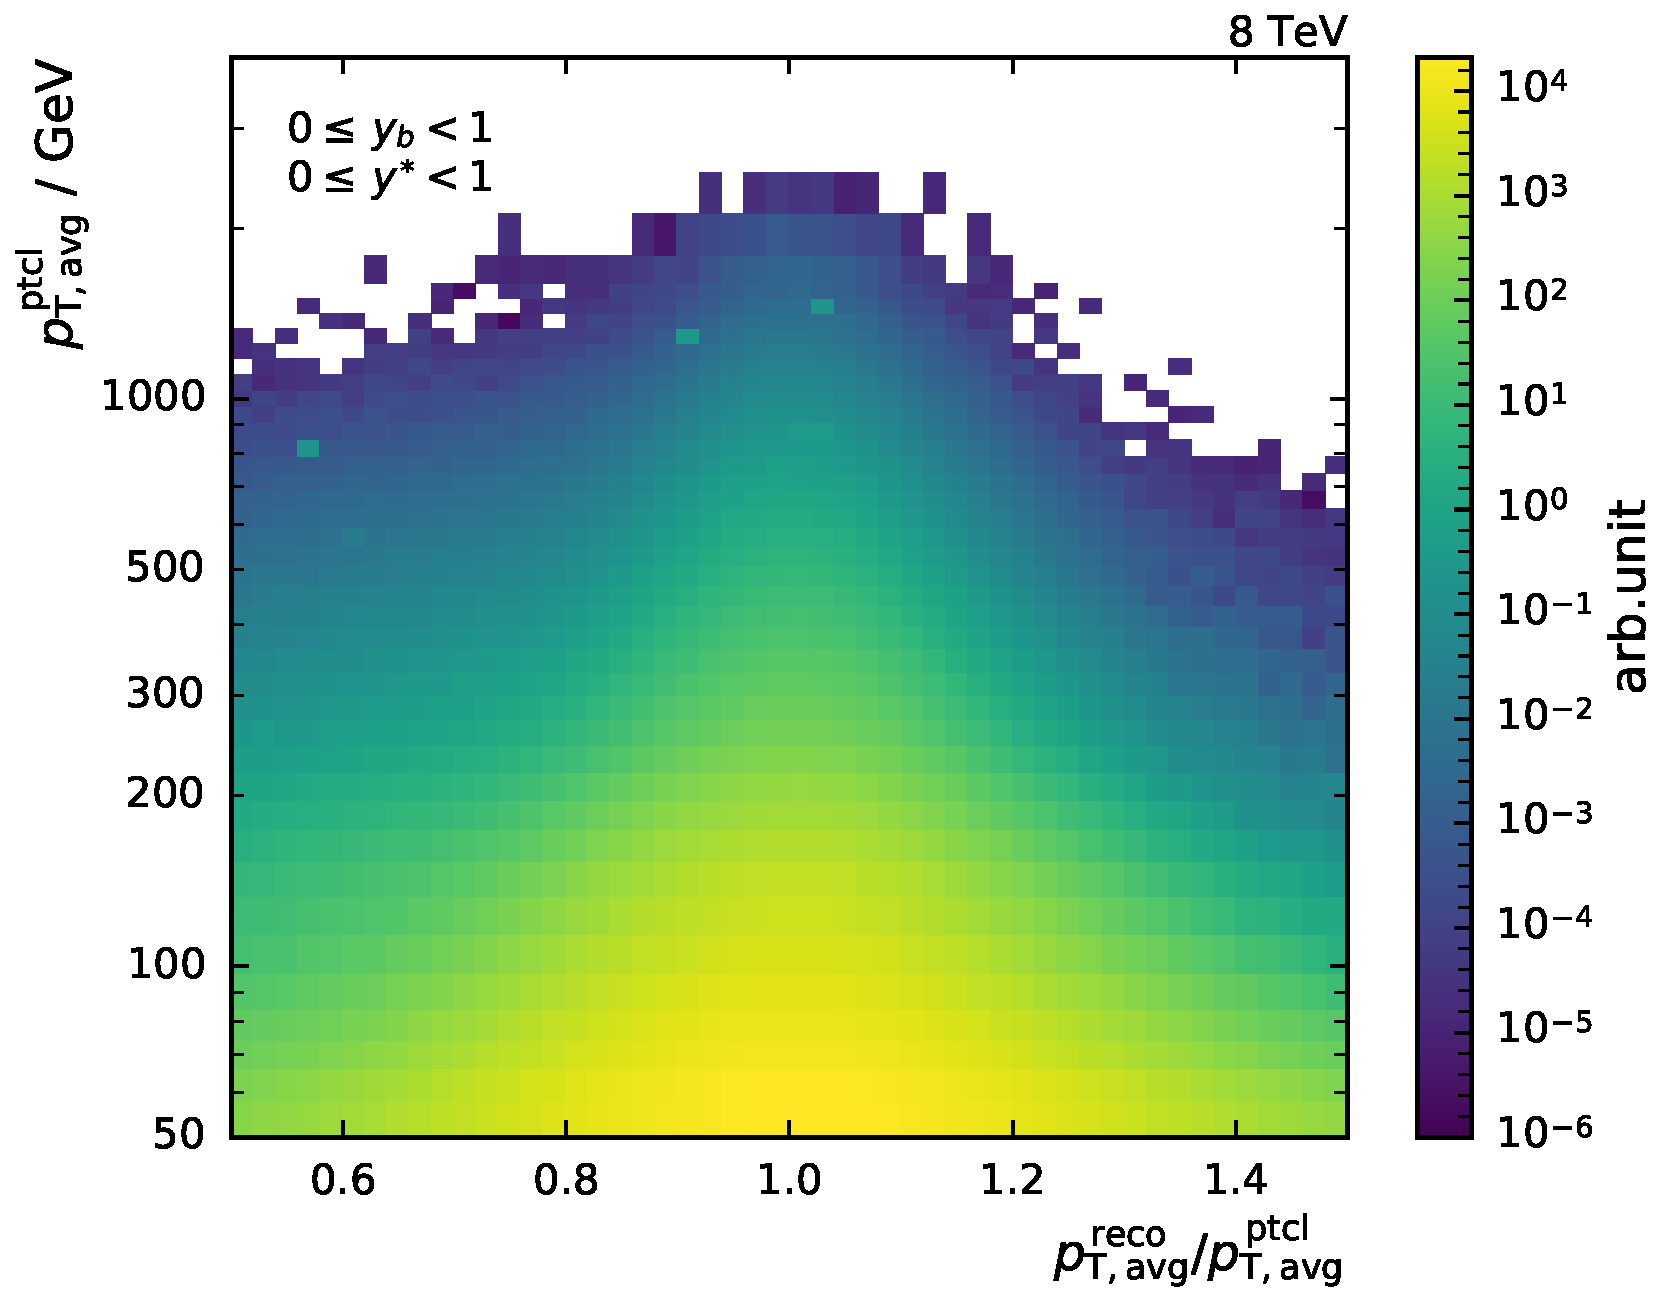
\includegraphics[width=0.45\textwidth]{figures/measurement/gen_vs_reco_vs_gen_ptavg_yb0ys0.pdf}\hfill
    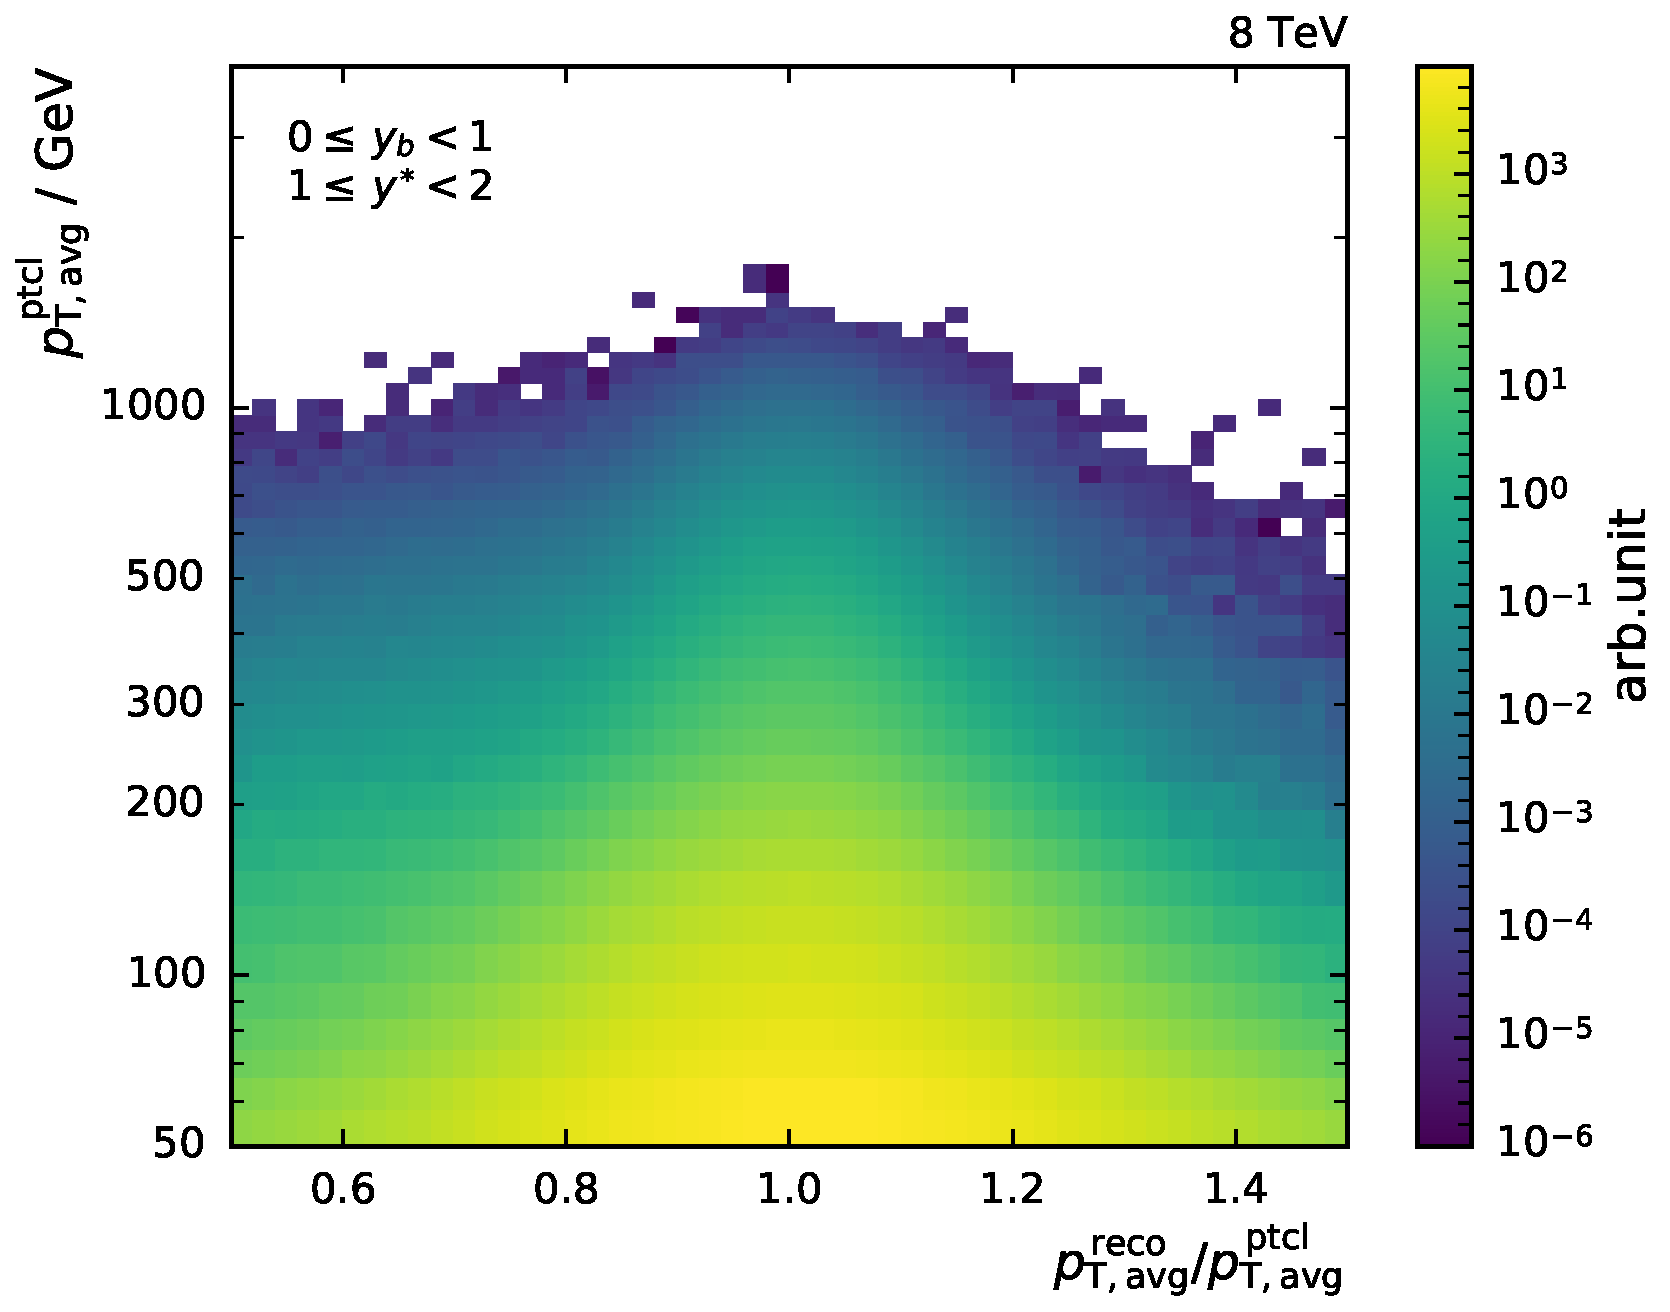
\includegraphics[width=0.45\textwidth]{figures/measurement/gen_vs_reco_vs_gen_ptavg_yb0ys1.pdf}
    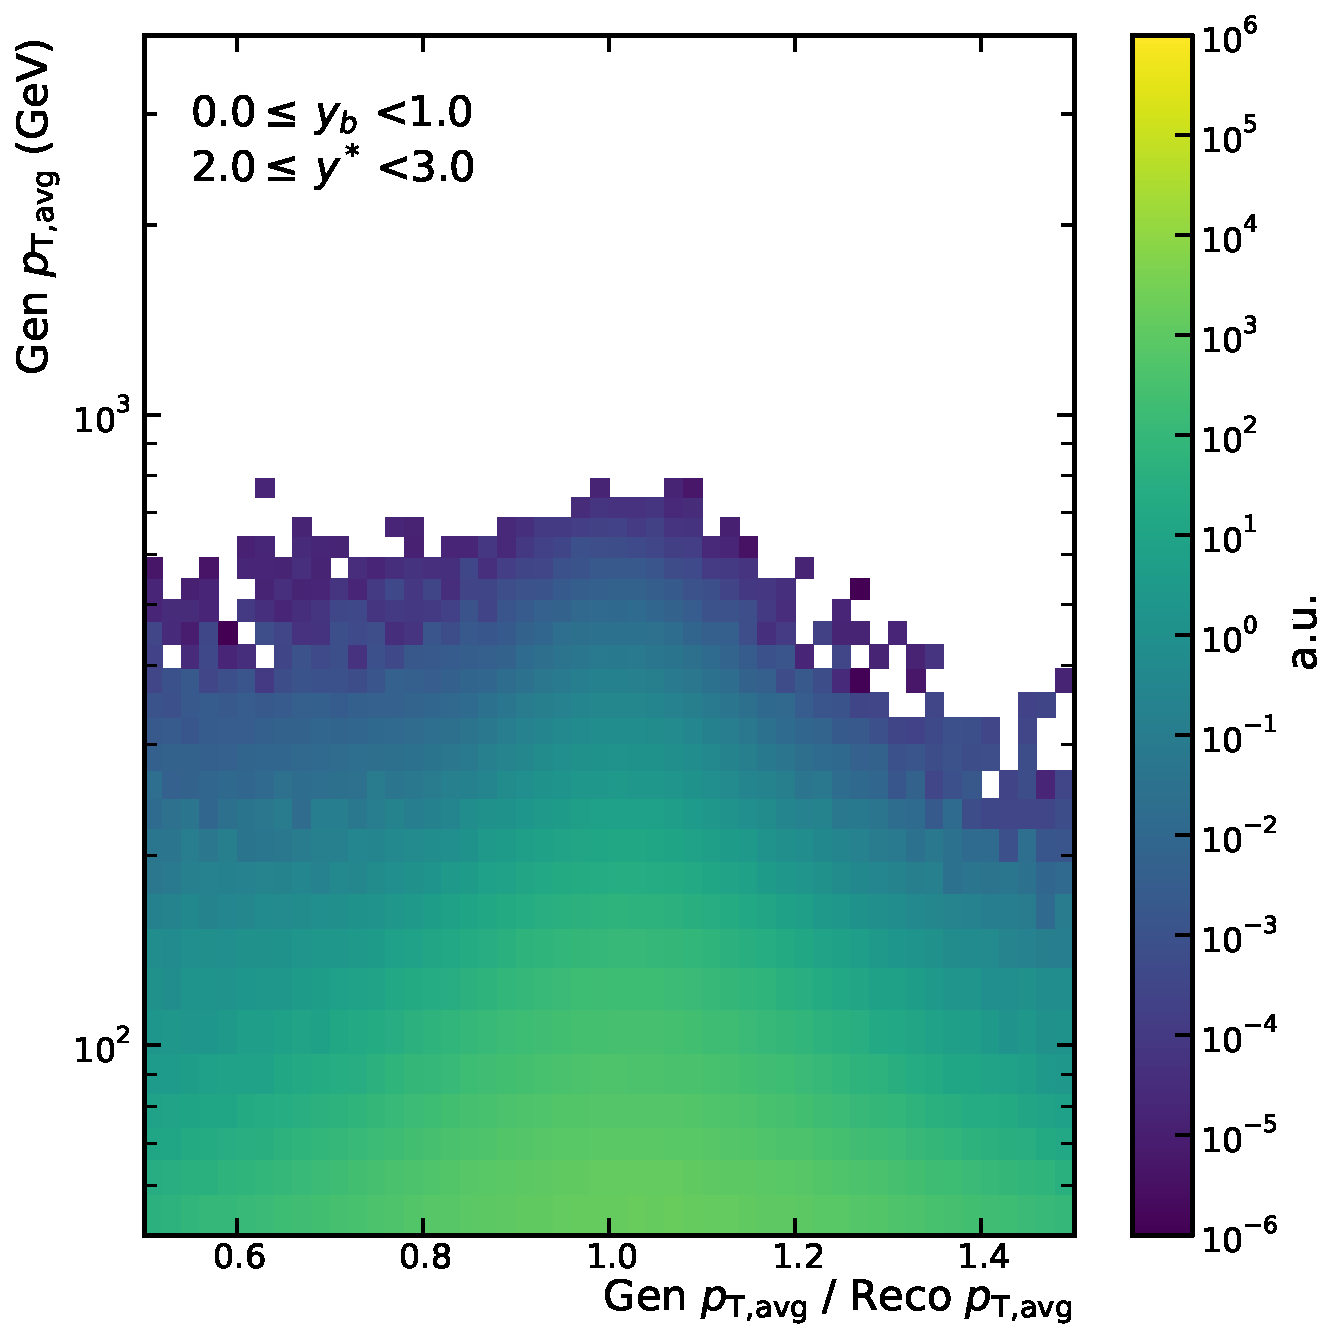
\includegraphics[width=0.45\textwidth]{figures/measurement/gen_vs_reco_vs_gen_ptavg_yb0ys2.pdf}\hfill
    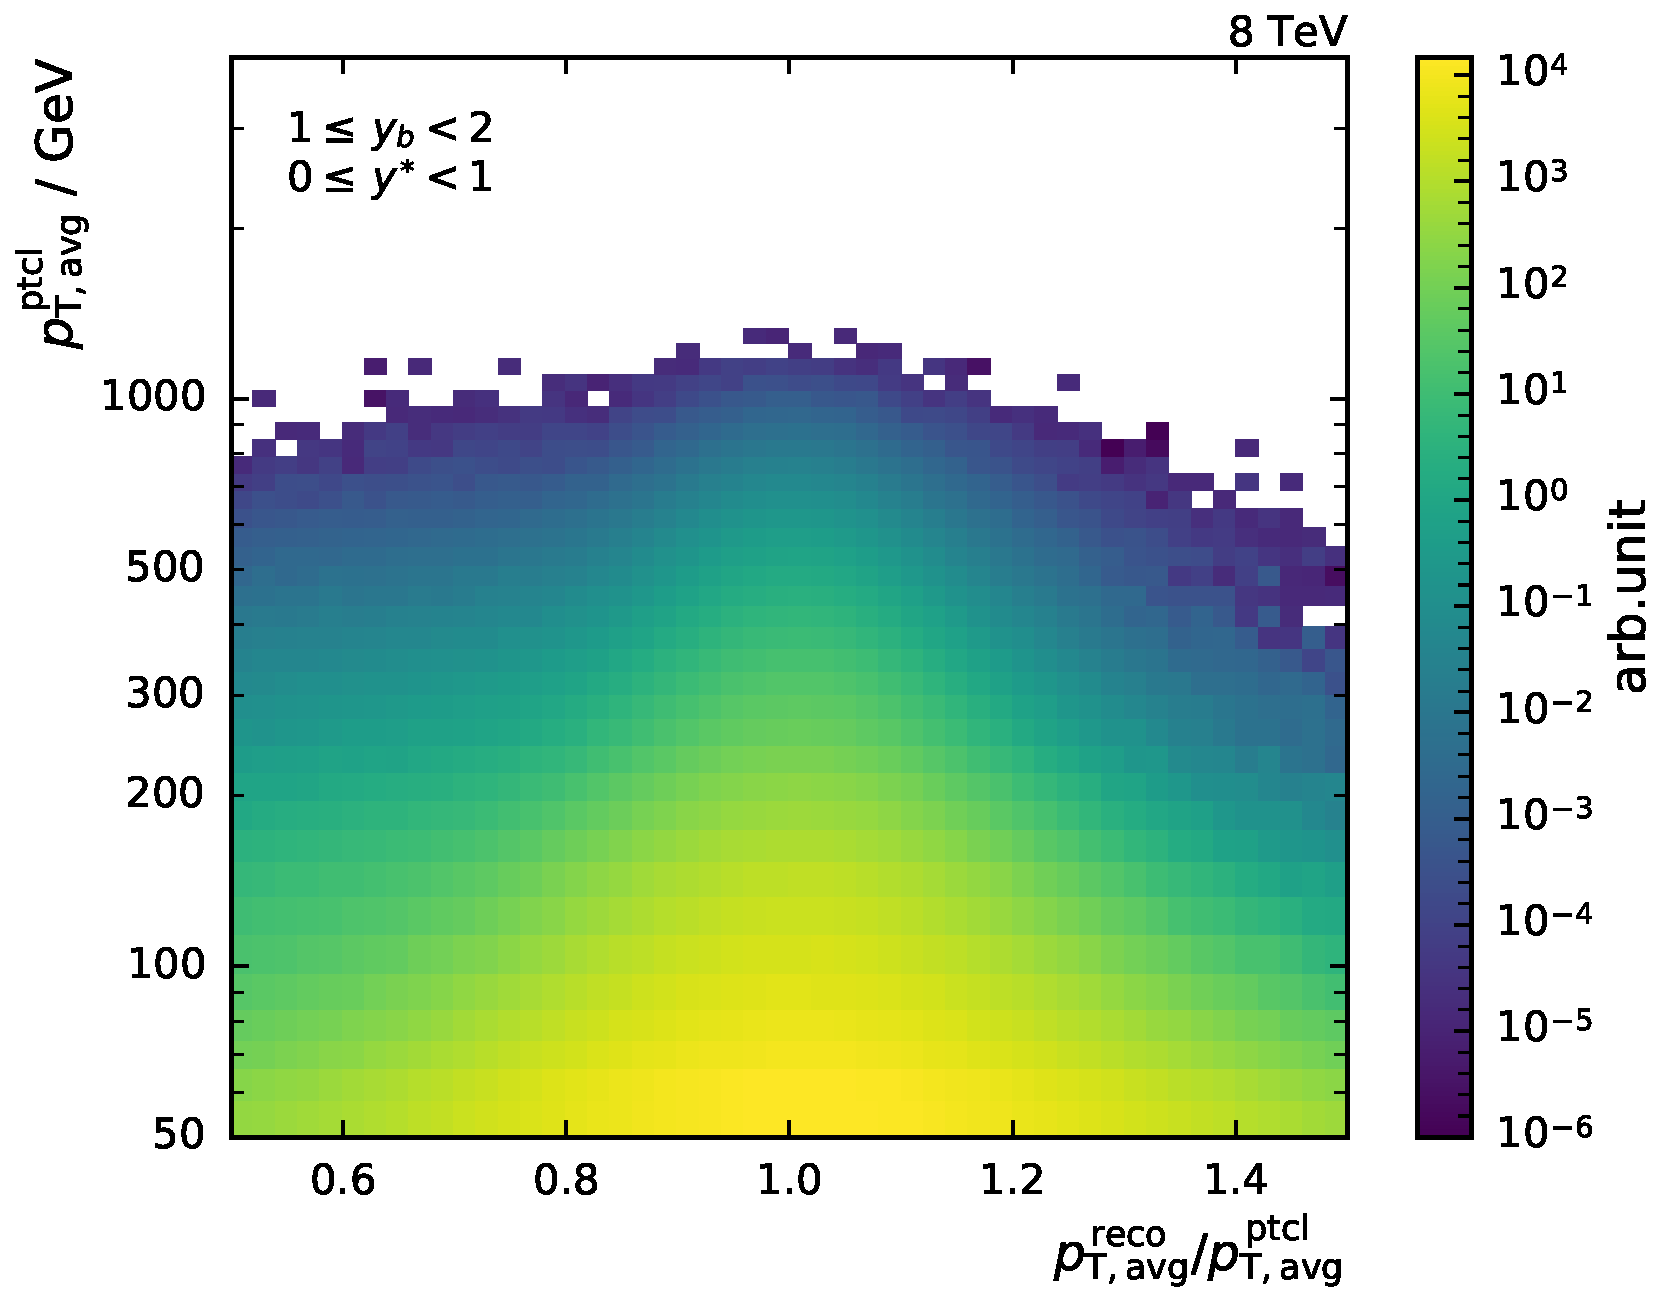
\includegraphics[width=0.45\textwidth]{figures/measurement/gen_vs_reco_vs_gen_ptavg_yb1ys0.pdf}
    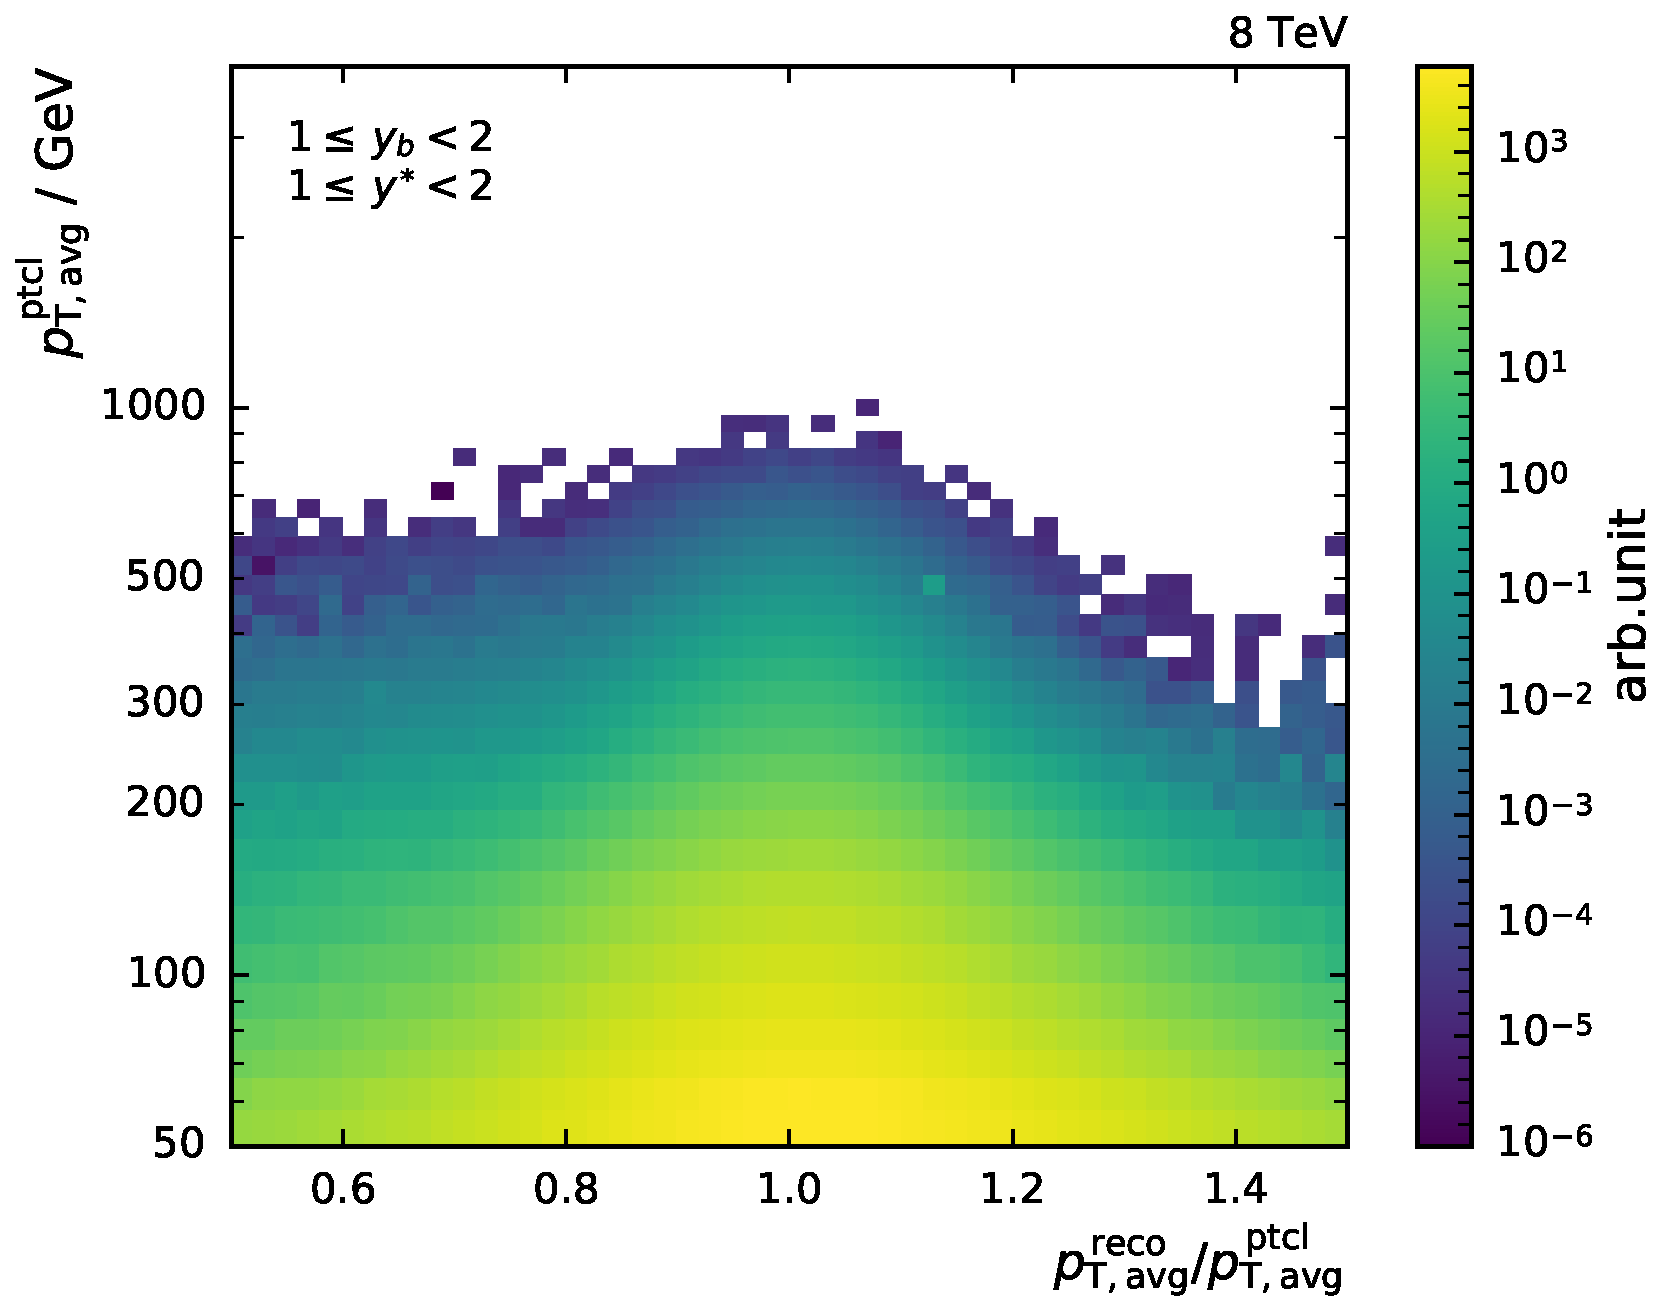
\includegraphics[width=0.45\textwidth]{figures/measurement/gen_vs_reco_vs_gen_ptavg_yb1ys1.pdf}\hfill
    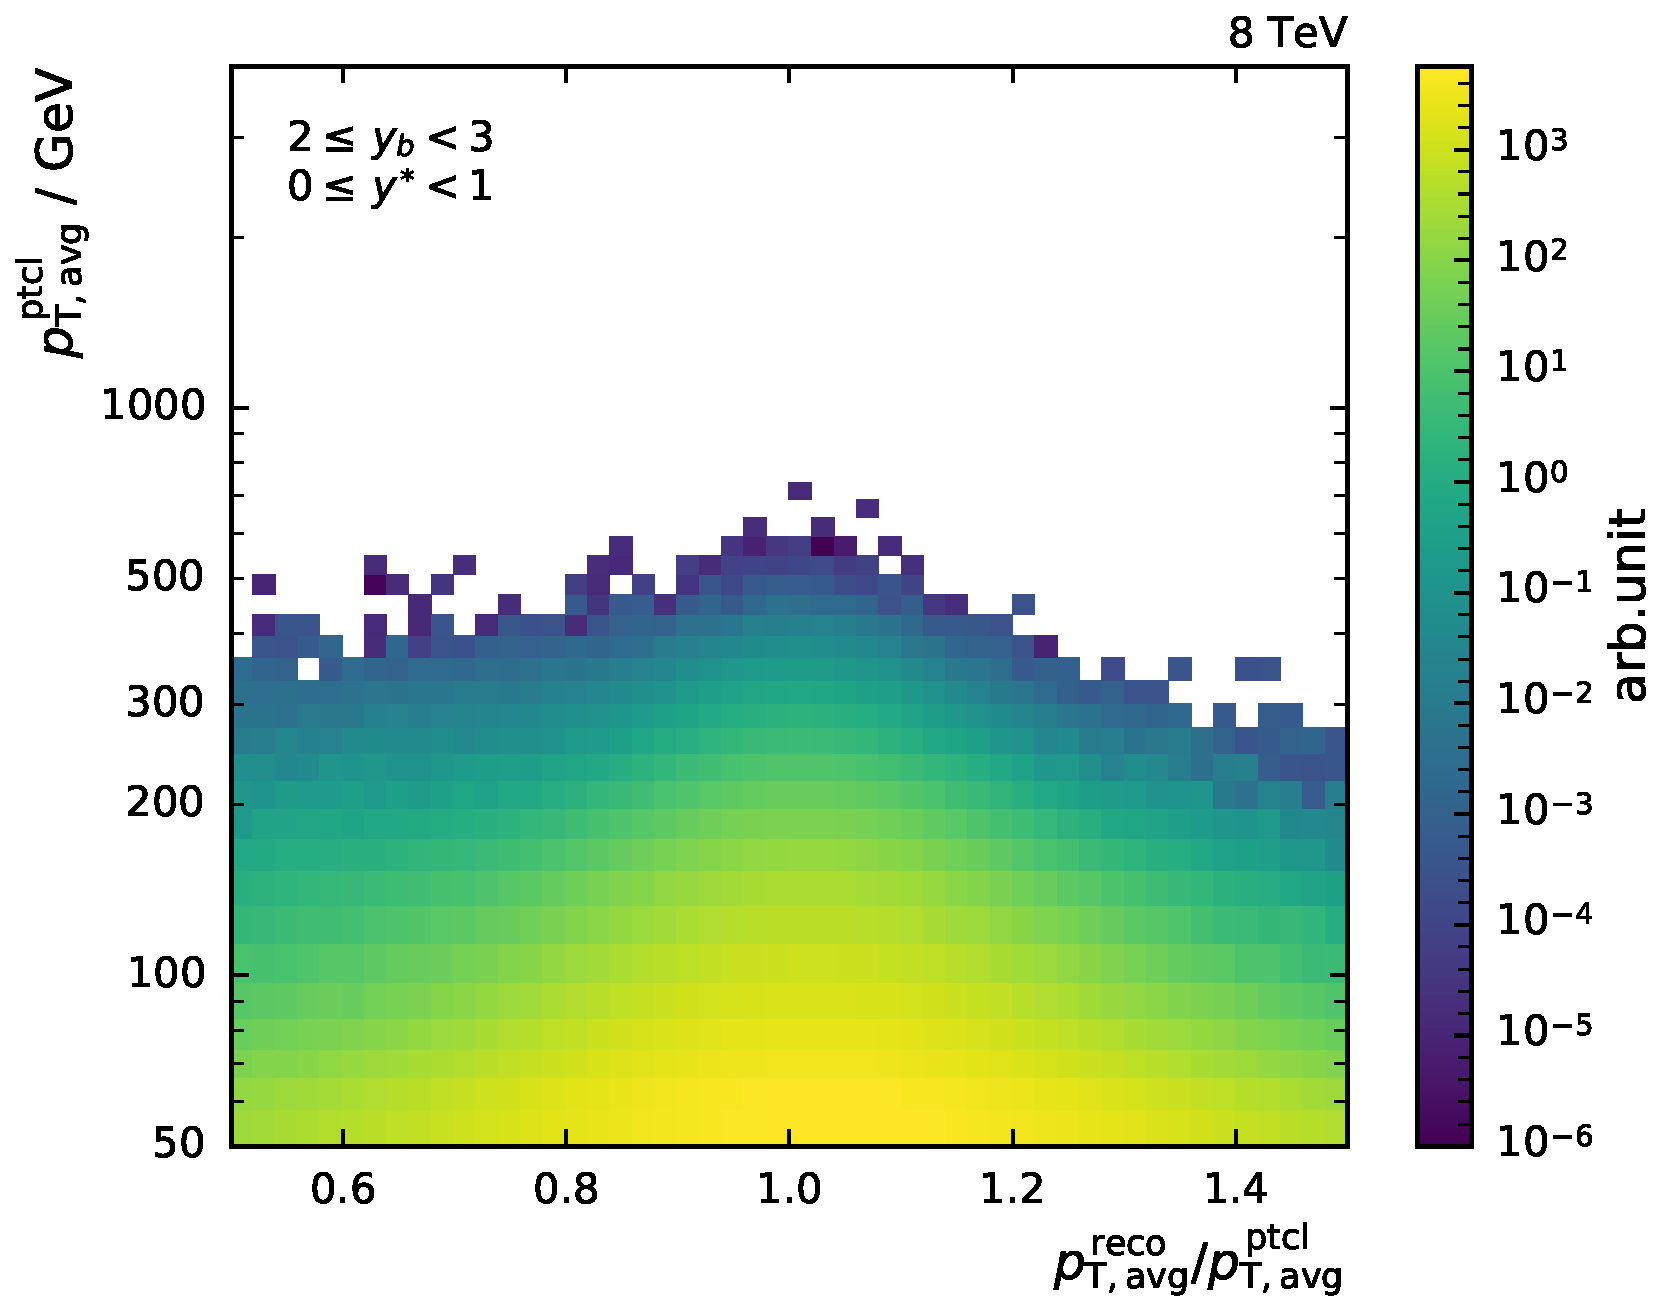
\includegraphics[width=0.45\textwidth]{figures/measurement/gen_vs_reco_vs_gen_ptavg_yb2ys0.pdf}
    \caption{Response matrix used for the unfolding procedure. The response matrices are obtained
            using the smearing method and are normalized to the number of gen events in each row to improve
            the readibility.}
    \label{fig:gen_vs_reco_over_gen}
\end{figure}

Figure~\ref{fig:resolution_bin} shows the distribution for one \ptavg bin. The
width is fitted using a gaussian function. The non-gaussian tails, visible in
the logarithmic representation, were found to not influence the resulting
resultion. The width of the distributions in each /ptavg is then shown as a
function of \ptavg. Figure~\ref{fig:resolution_ptavg} shows the final relative
resolution for each \ystar and \yboost bin. The relative resolution is described
by a modified version of the NSC formula.

\begin{equation}
    \frac{\sigma_{\text{ptavg}}}{\ptavg} (\ptavg) = \sqrt{\sgn{N} \left(\frac{N}{\ptavg}\right)^2 + \left(\frac{\ptavg}{\text{GeV}}\right)^s \frac{S^2}{\ptavg} + C^2 }
    \label{eq:resolution}
\end{equation}

\begin{figure}[htbp]
    \centering
    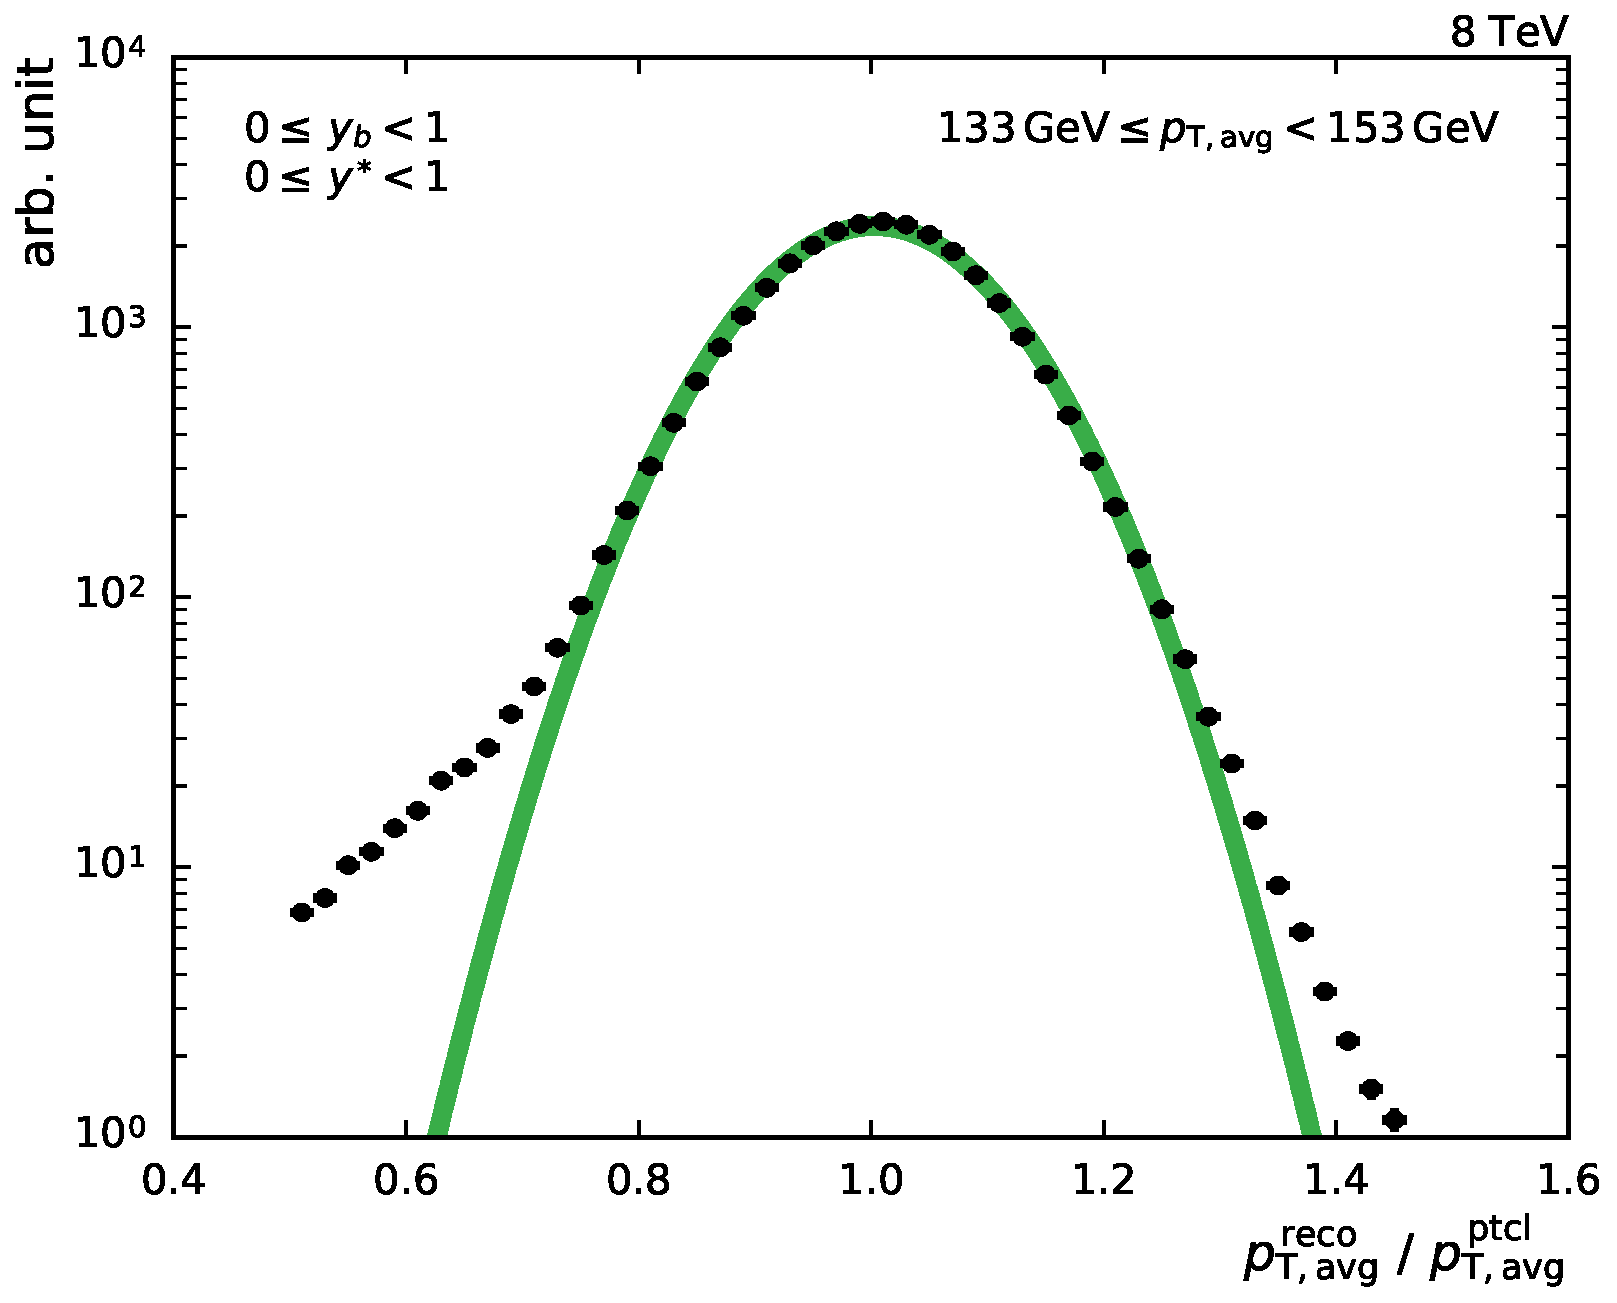
\includegraphics[width=0.5\textwidth]{figures/measurement/resolution_yb0ys0_bin10.pdf}
    \caption{Dijet \ptavg resolution}
    \label{fig:resolution_bin}
\end{figure}


\begin{figure}[htbp]
    \centering
    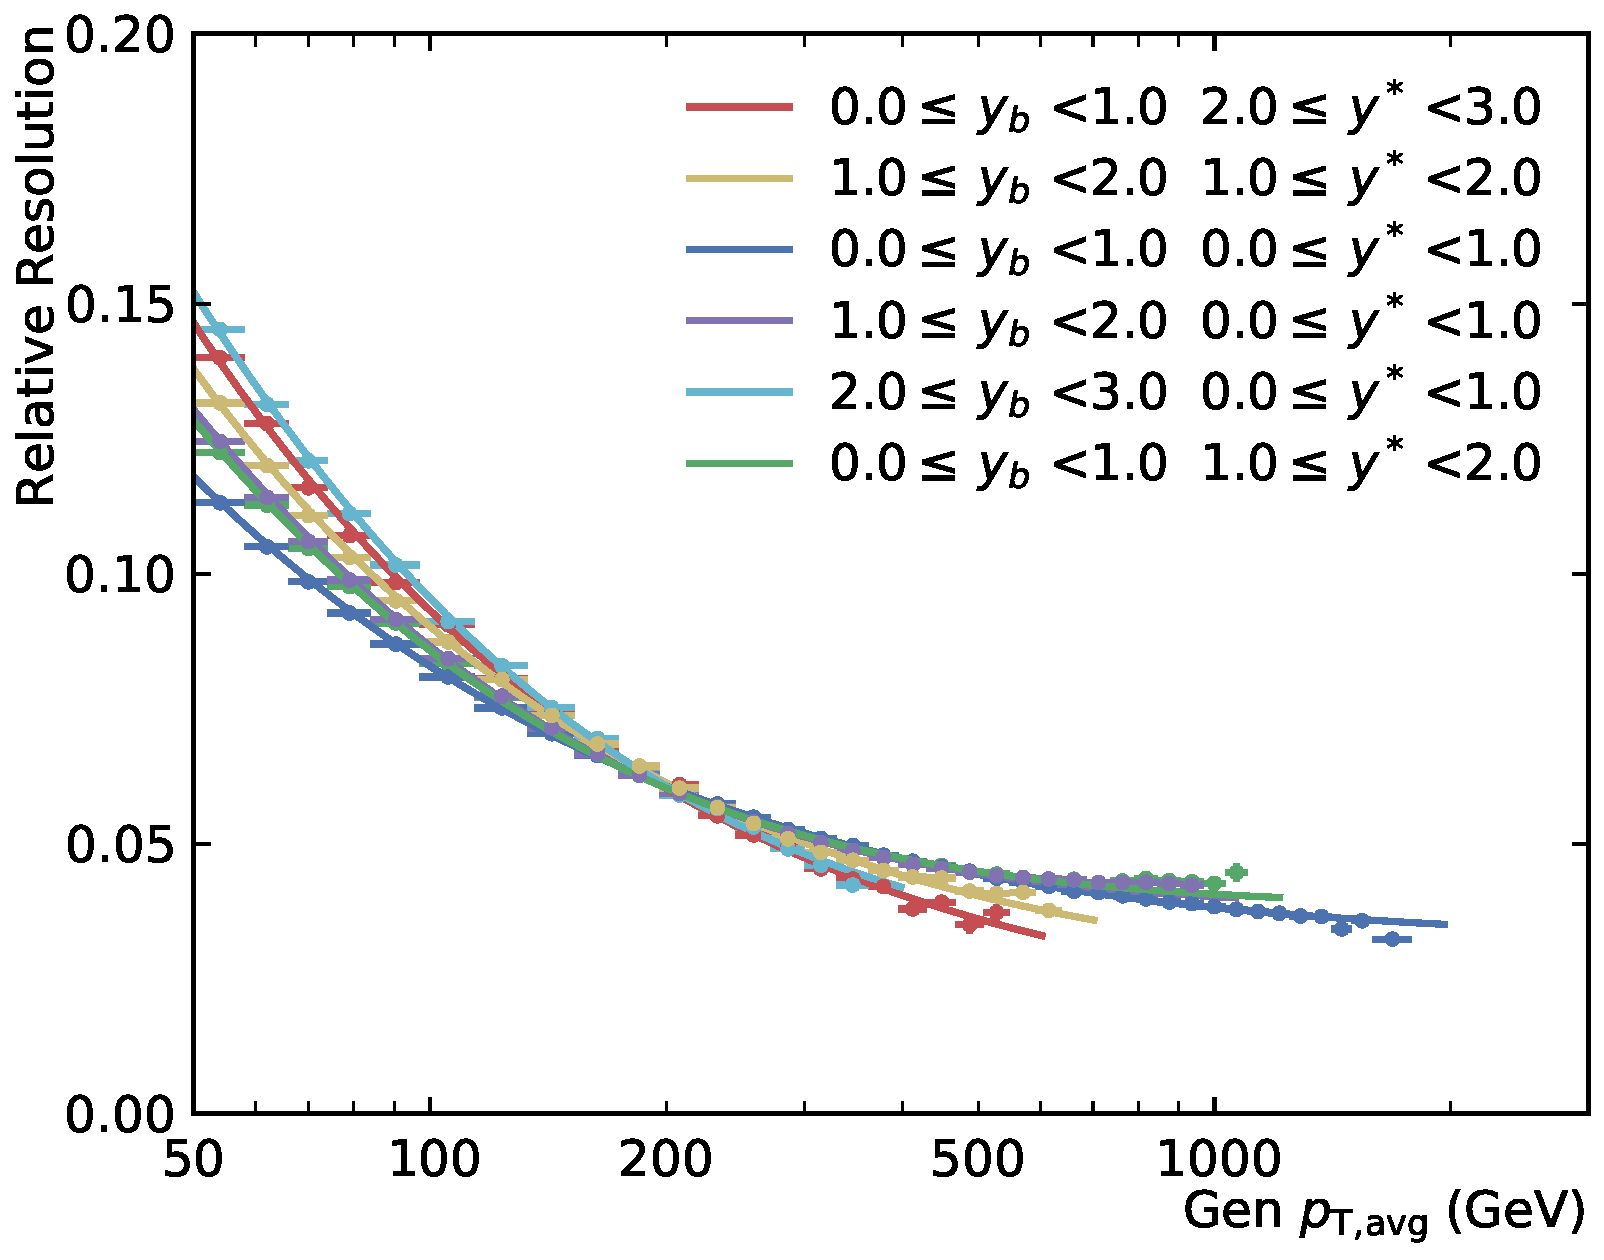
\includegraphics[width=0.5\textwidth]{figures/measurement/resolution_ptavg.pdf}
    \caption{Dijet \ptavg resolution}
    \label{fig:resolution_ptavg}
\end{figure}

The formula is based on the usual NSC formula which describes the resolution in
terms of noise $N$, a stochastic component $S$ and a constant term $C$.
Especially in the low-\pt region in which the tracking has a non-negligible
influence on the resolution due to the particle flow algorithm, a slightly
better fit is obtained by using the modified resolution
formula~\ref{eq:resolution}. Table~\ref{tab:resolution_parameters} gives the
parameters of the fit in each bin of the measurement.

\begin{table}[htbp]
    \centering
    \begin{tabular}{cccccr}
        \toprule
         \yboost & \ystar & N      & S     & C      & s\\\midrule
         0 -- 1  & 0 -- 1 & -6.26  & 3.62  & 0.05   & -0.43\\
         0 -- 1  & 1 -- 2 & -25.96 & 23.05 & 0.05   & -0.91\\
         0 -- 1  & 2 -- 3 & -6.56  & 4.02  & -0.017 & -0.43\\
         1 -- 2  & 0 -- 1 & -28.33 & 25.51 & 0.05   & -0.92\\
         1 -- 2  & 1 -- 2 & -5.79  & 3.13  & 0.03   & -0.35\\
         2 -- 3  & 0 -- 1 & -7.12  & 3.967 & 0.00   & -0.41\\\hline
            \bottomrule
    \end{tabular}
    \caption{The parameters of the resolution fit are shown for each bin in \ystar and \yboost.}
    \label{tab:resolution_parameters}
\end{table}

\section{Unfolding of the Measurement}

The final goal is the comparison of the triple-differential dijet cross section
with higher-order QCD calculations. Due to the finite detector acceptance and resolution
the measured spectrum is smeared causing differences between the true dijet \ptavg distribution
and the measured distribution. To accomplish that goal, the measurement has
to be unfolded to yield the result at particle level. Thus all future Monte-Carlo event
generators can be easily compared with this measurement without needing to apply
the detector simulation.

In this analysis, the iterative d'Agostini algorithm~\cite{DAgostini:1994zf} which is
implemented in the RooUnfold~\cite{Adye:2011gm} package is used. The unfolding
process is regularized by the number of interation steps in this algorithm. A
higher number of iterations yields a better reduced \chisq but also increases
the uncertainty and introduces larger bin-by-bin fluctuations and correlations.
The regularization was optimized using a Monte-Carlo data sample and best
results with low bin-by-bin correlations and a low \chisq were achieved using
four iterations in the unfolding algorithm.

In principal, the response matrix for the unfolding algorithm can be directly
filled using the Monte-Carlo generated events containing the thue and measured
information. However this method has several drawbacks. The LO prediction not
neccesarily describes the shape of the distribution in all cases. Additionally
the limited number of events in the Monte-Carlo sample, especially at high
rapidities and high transverse momentum, introduces large statistical
fluctuations in the response matrix. Because of these undesired effects a
different stategy is employed to populate the response matrix.

Based on the good description of the data spectrum by NLO predictions, a forward
smearing is applied. At first, the NLO prediction obtained with the CT14-NLO PDF
set and corrected for non-perturbative effects, is fitted using the function

\begin{equation}
    f(\ptavg) = A_0 \left(
    \frac{\ptavg}{A_3}\right)^{-A_1}\left(1-\frac{\ptavg}{A_3}\right)^{A_2}
\end{equation}

Using a Toy MC method a flat \ptavg spectrum is generated, which is weighted
according to the NLO distribution. The distribution of this generated sample
resembles the fastNLO cross section prediction and is used as the true \ptavg
spectrum. The generated events are smeared using the resolution function
measured in Section~\ref{sec:resolution}. The generation of these Monte-Carlo
toy events is very fast, and the response matrices are filled with around 100
million events each resulting in negligible statistical fluctuations.
Figure~\ref{fig:res_matrix} shows the response matrices used in the unfolding
process. The matrices in the figure are normalized to number of gen events in
each row to improve the readibility. The response matrices are diagonal with
small off-diagonal migrations between close-by \ptavg bins.

\begin{figure}[htp]
    \centering
    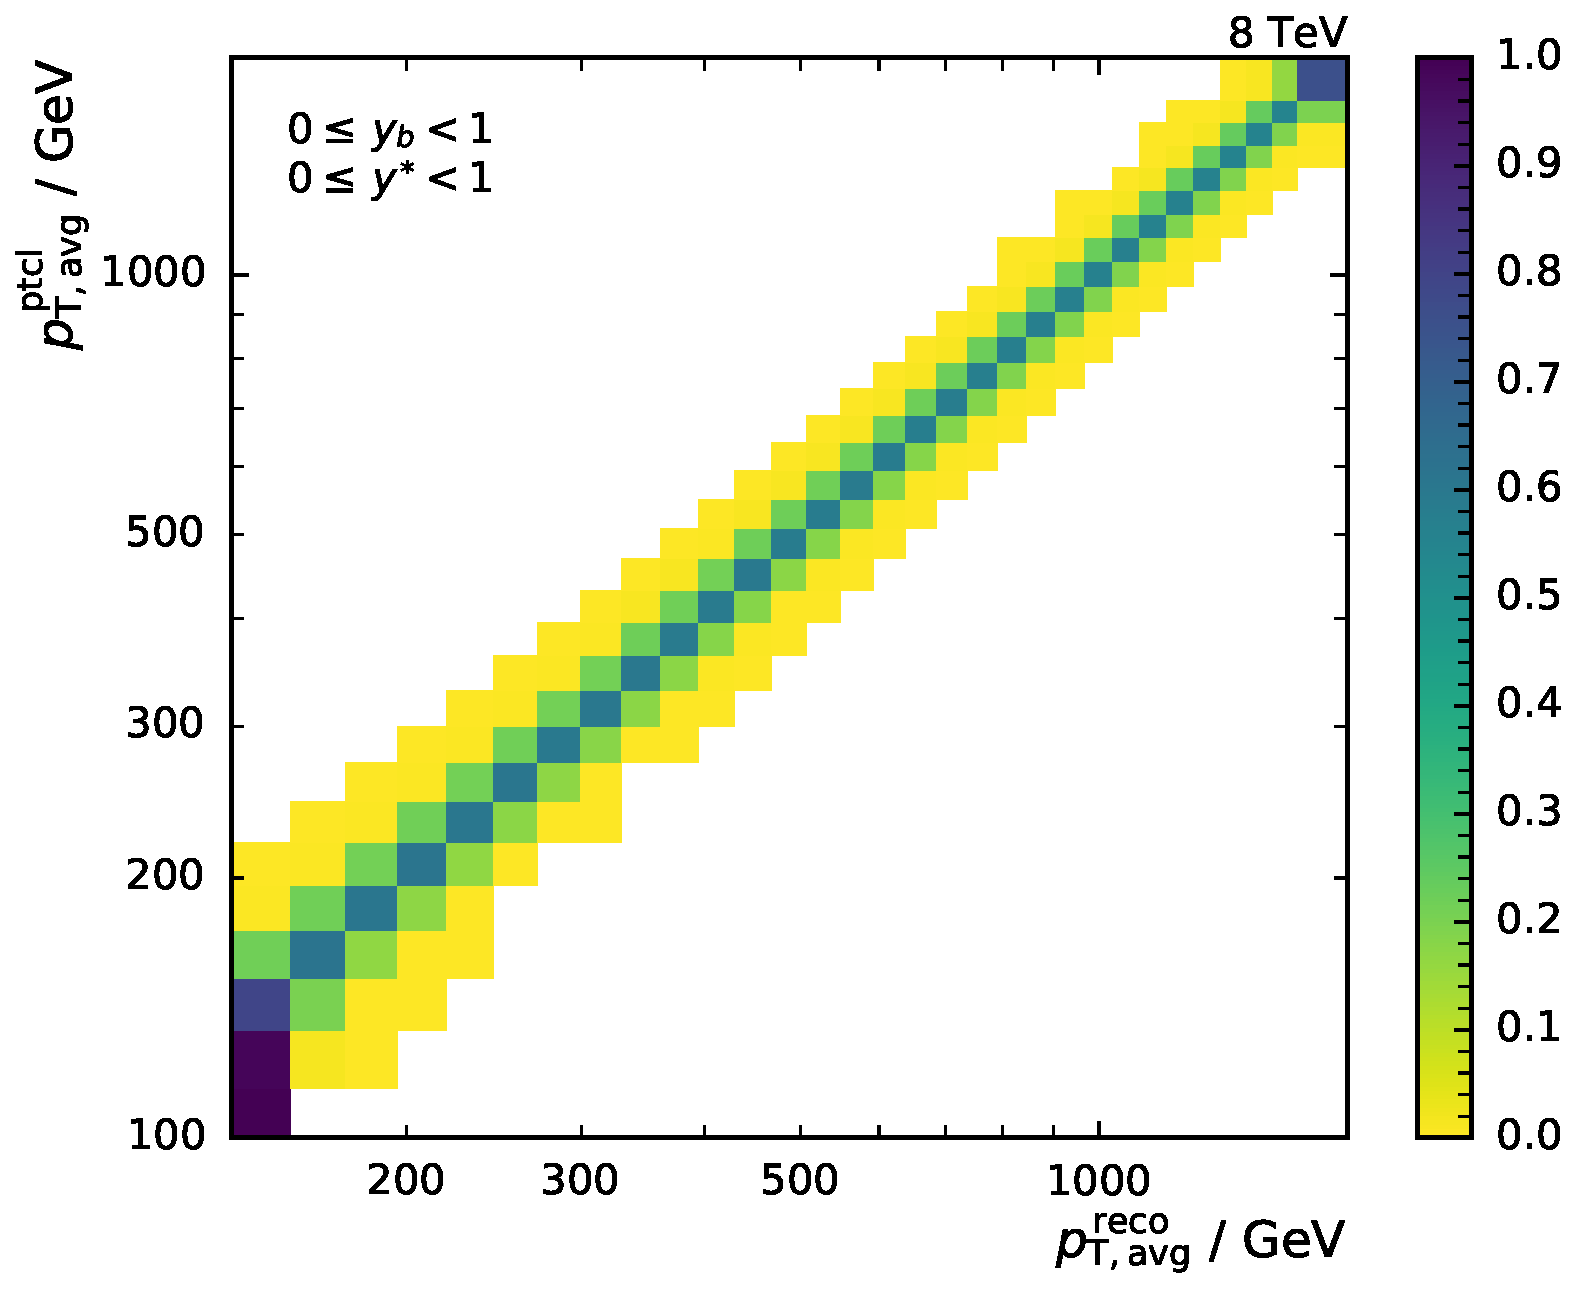
\includegraphics[width=0.45\textwidth]{figures/measurement/res_matrix_ptavg_normalized_yb0ys0.pdf}\hfill
    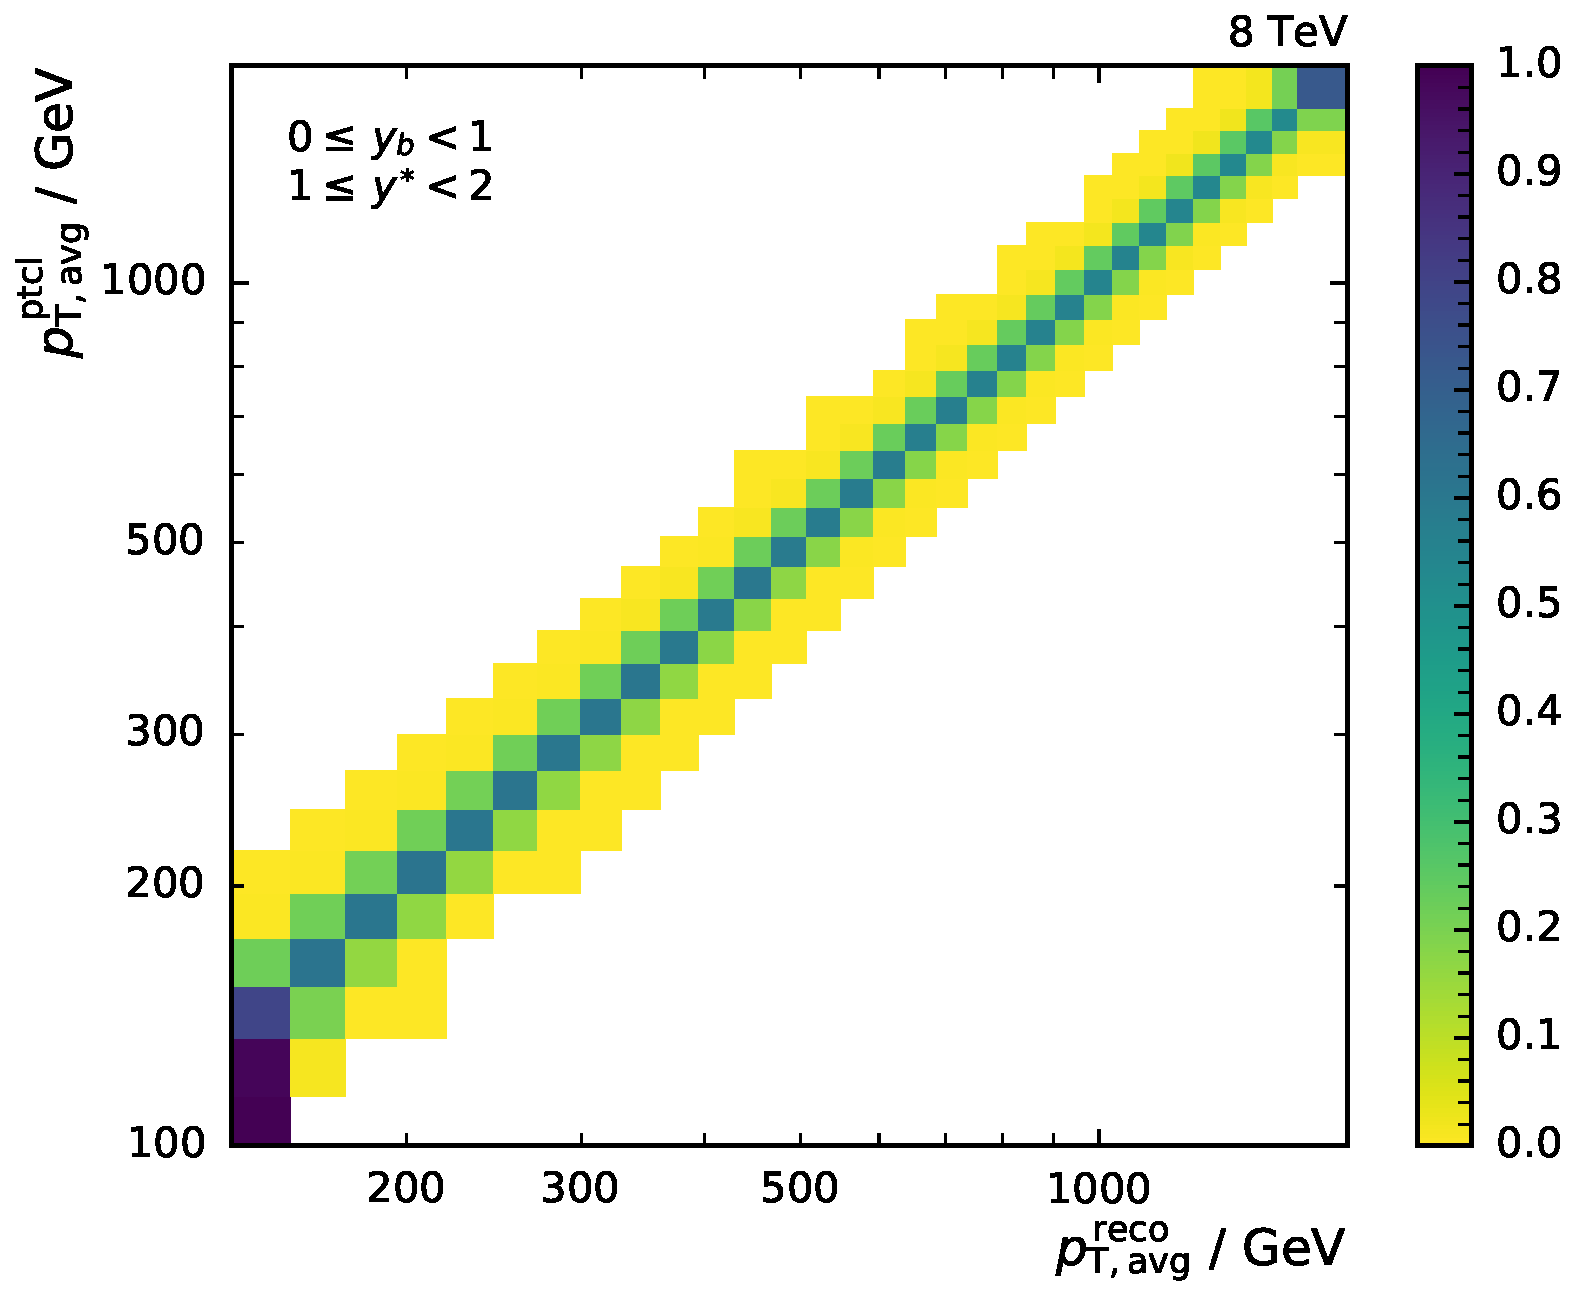
\includegraphics[width=0.45\textwidth]{figures/measurement/res_matrix_ptavg_normalized_yb0ys1.pdf}
    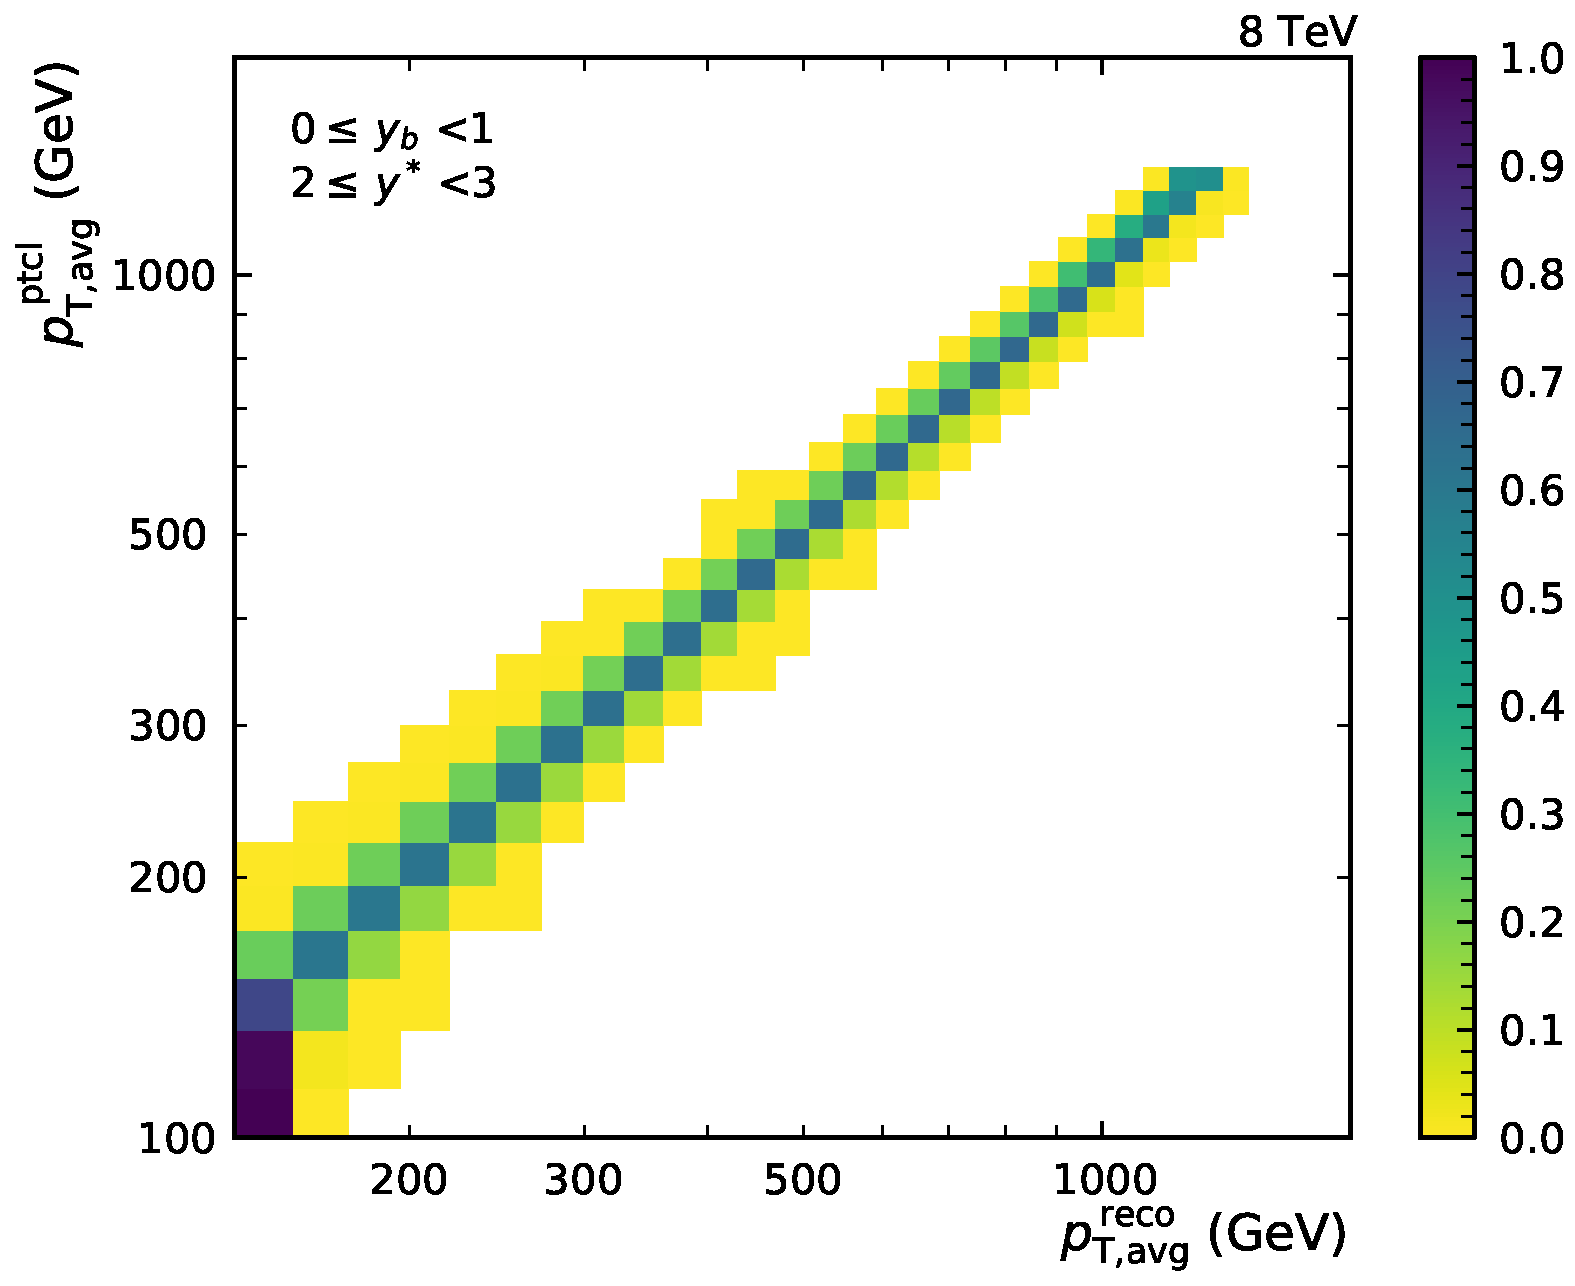
\includegraphics[width=0.45\textwidth]{figures/measurement/res_matrix_ptavg_normalized_yb0ys2.pdf}\hfill
    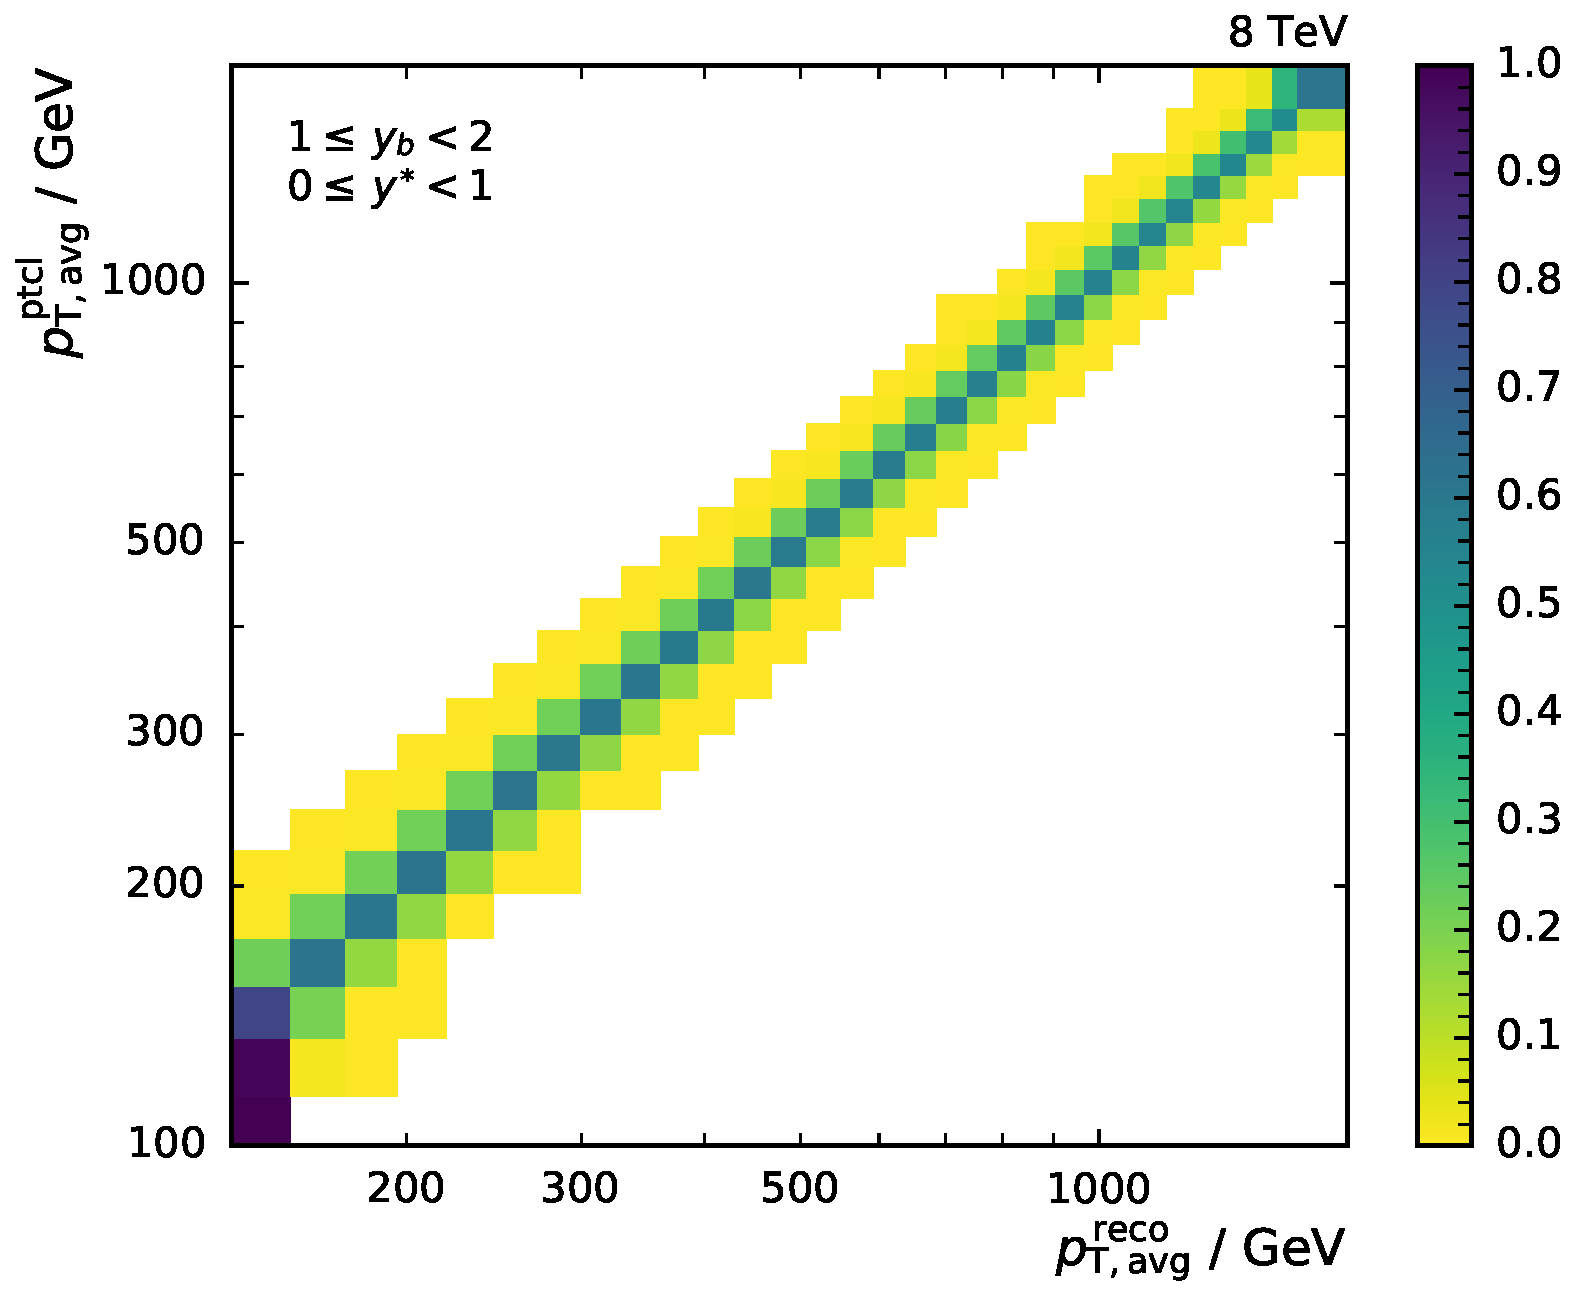
\includegraphics[width=0.45\textwidth]{figures/measurement/res_matrix_ptavg_normalized_yb1ys0.pdf}
    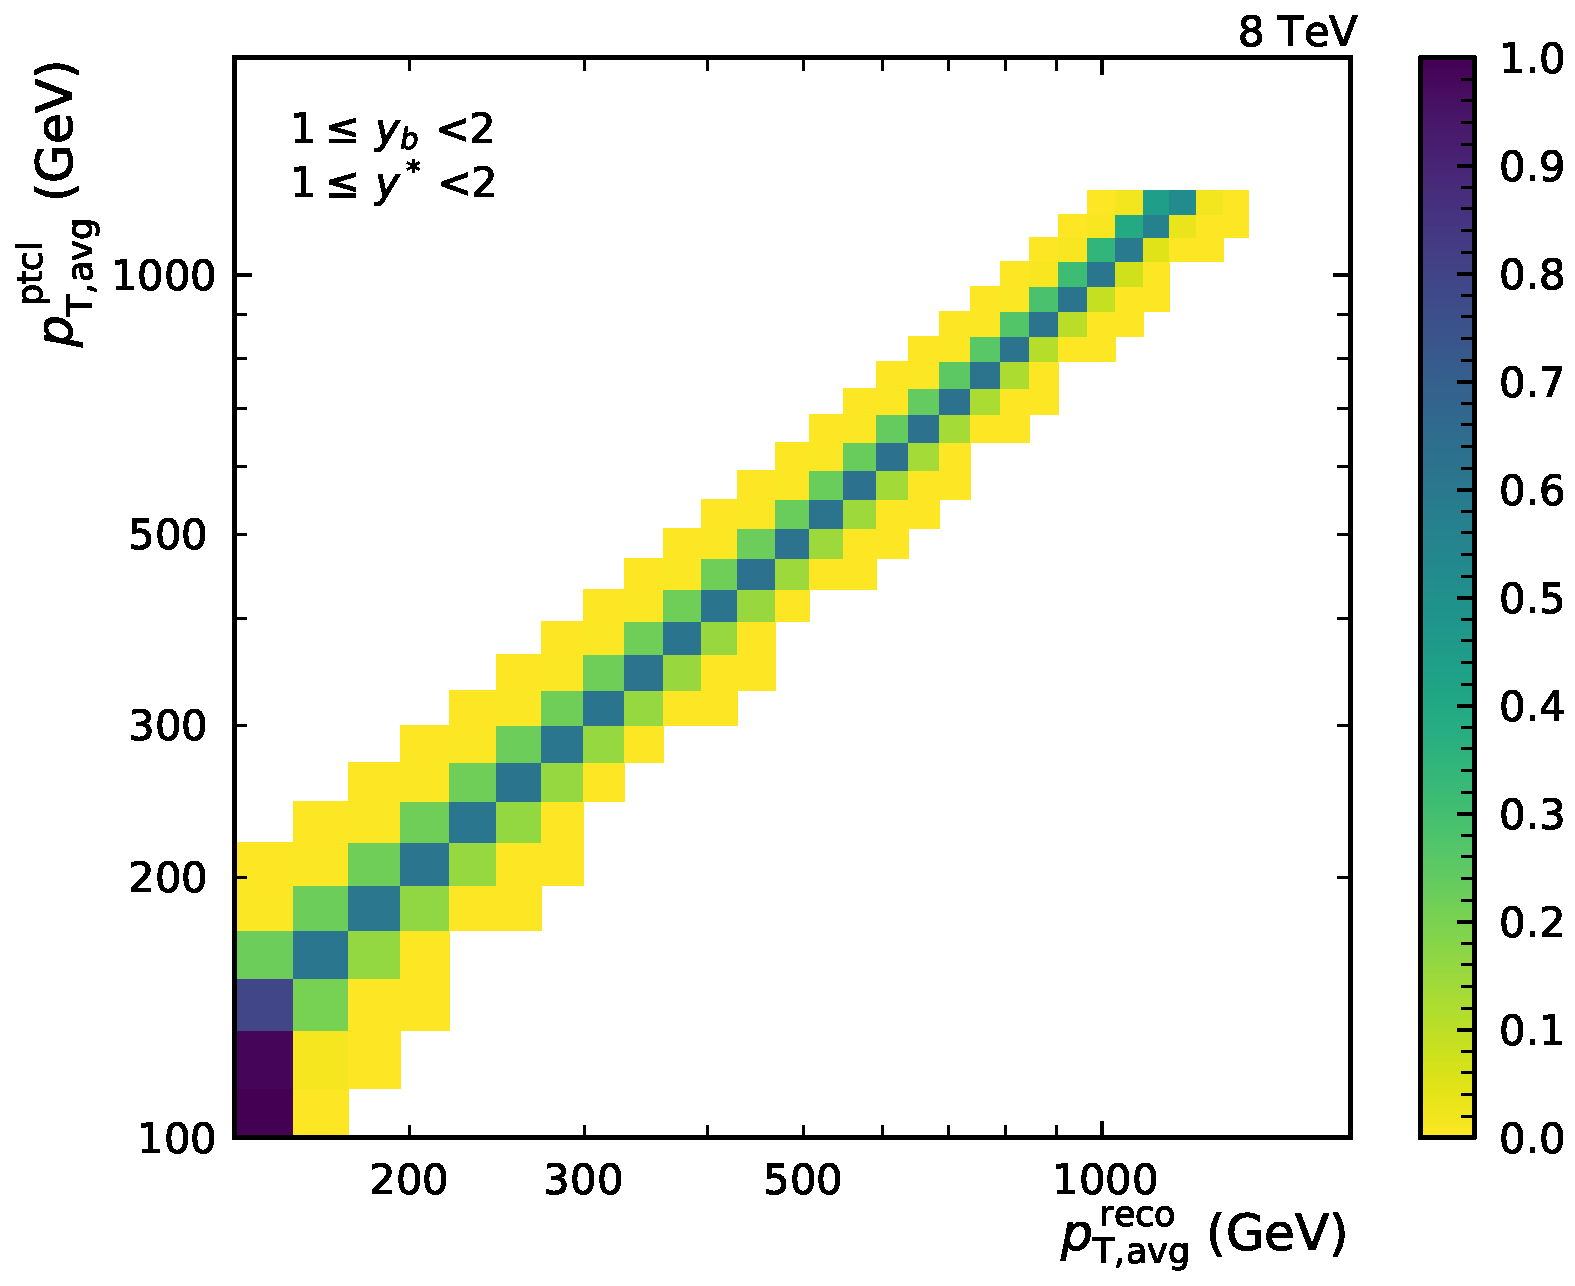
\includegraphics[width=0.45\textwidth]{figures/measurement/res_matrix_ptavg_normalized_yb1ys1.pdf}\hfill
    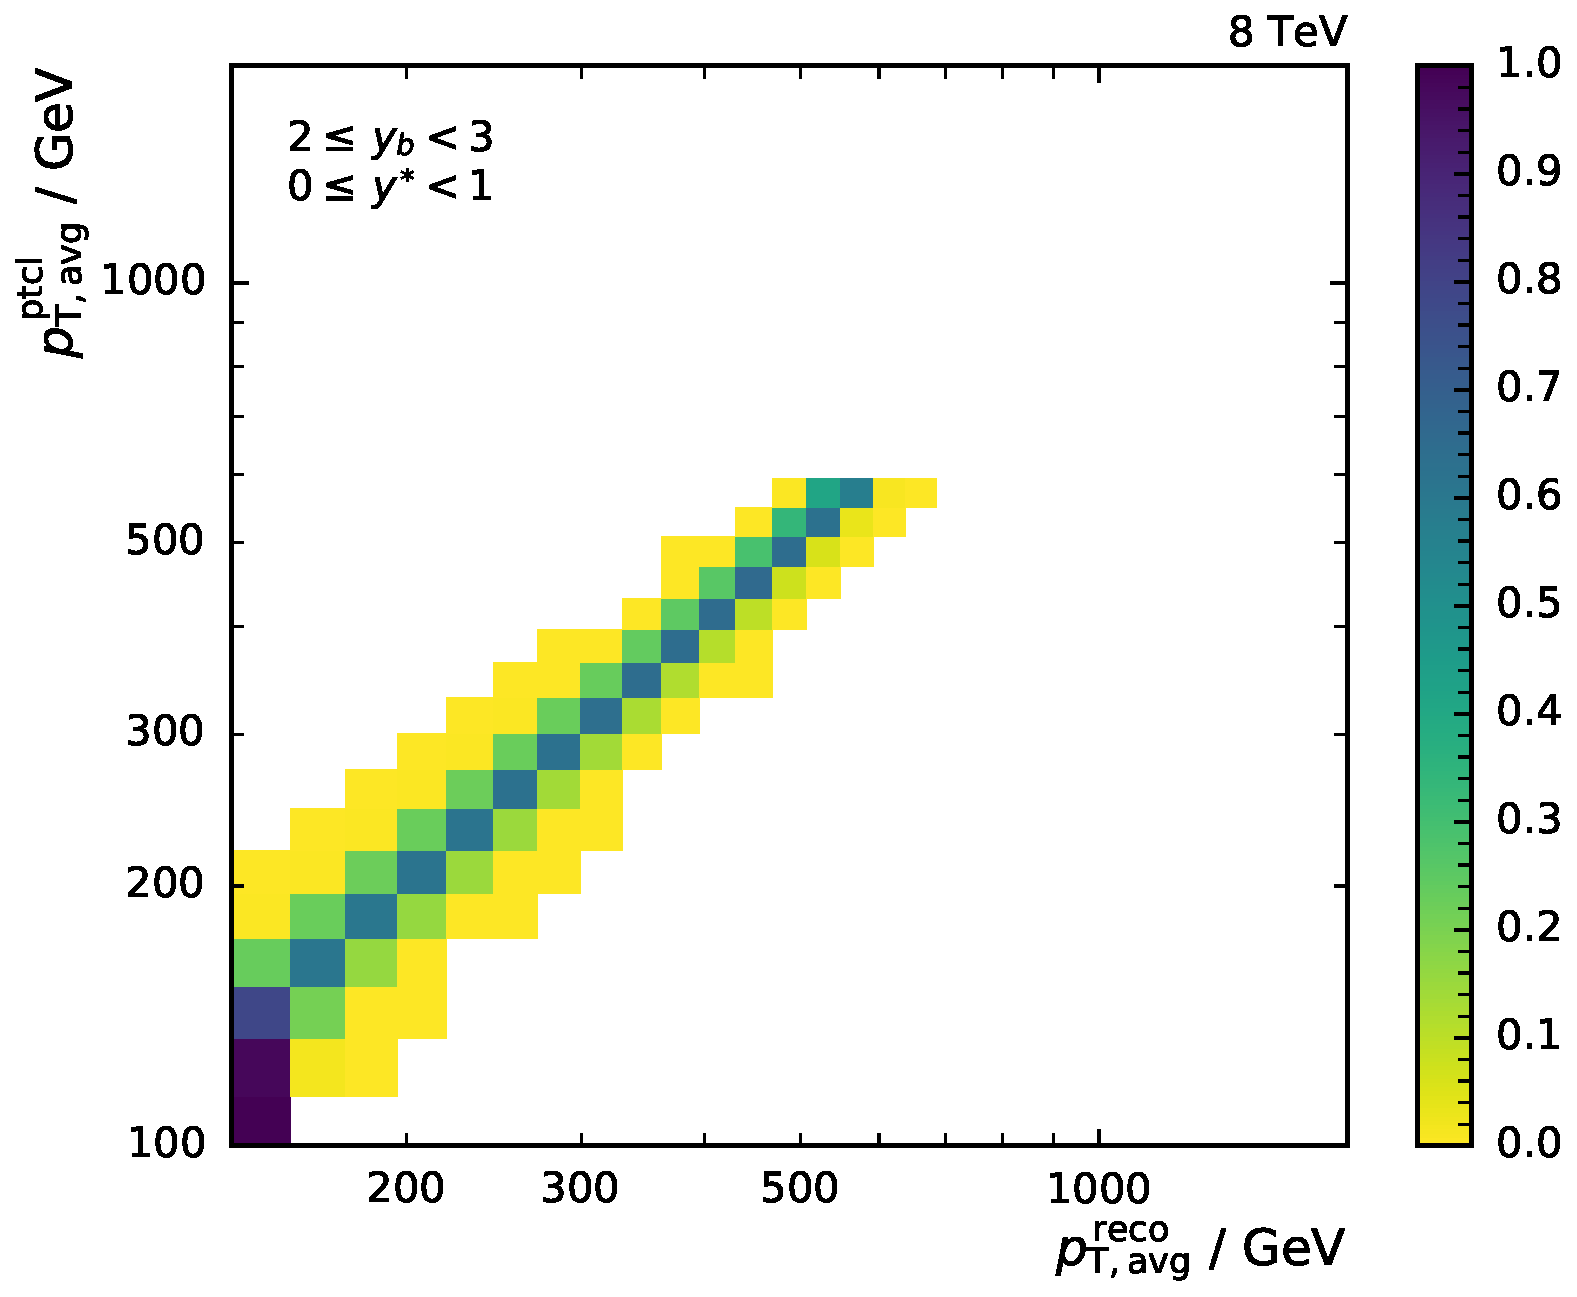
\includegraphics[width=0.45\textwidth]{figures/measurement/res_matrix_ptavg_normalized_yb2ys0.pdf}
    \caption{Response matrix used for the unfolding procedure. The response matrices are obtained
            using the smearing method and are normalized to the number of gen events in each row to improve
            the readibility.}
    \label{fig:res_matrix}
\end{figure}

A closure test was performed by applying the unfolding using response matrices
filled directly from the Monte-Carlo samples and from the generated and smeared
toy events. It was found that the results agree in both cases within statistical
uncertainties.

Additionally it was studied that the bin-by-bin migration between phase space
bins in \ystar and \yboost are small and the effects neglibible. Thereby it is
justified to perform the unfolding in each \ystar and \yboost bin separately and
to not perform a three-dimensional unfolding which is much more cumbersome.

The statistical uncertainties of the data distributions are propagated through
the unfolding procedure using toy experiments. The procedure as well as the
results are discussed in detail in Sec.~\ref{sec:stat_unf_uncert}.


\section{Experimental Uncertainties}

This section presents all experimental uncertainties, which affect the
measurement.  The luminosity uncertainty affects the
overall normalization of the cross section measurement. The dominant source of
uncertainty arises from the jet energy corrections which is split into 25
% separate sources of uncertainty. Table~\ref{tab:exp_uncerts} gives an overview
of the different sources of uncertainty and their influence on the measurement

% \todo{table exp uncertainties}

\subsection {Uncertainty on Luminosity Measurement}

As discussed in Sec.~\ref{sec:lumi_measurement}, the luminosity is measured from
the number of clusters in the silicon pixel detector. The integrated luminosity
for the selected data in the 2012 LHC run is determined to be \SI{19.71}{\per
\femto \barn}. 

The uncertainty on the luminosity measurement for the 2012 LHC run is estimated
to be 2.5\% (syst.) and 0.5\% (stat.)~\cite{CMS-PAS-LUM-13-001}. The luminosity
uncertainty afffects the normalization of any absolute cross section measurement
and is therefore taken into account.

\subsection{Unfolding and Statistical Uncertainty}
\label{sec:stat_unf_uncert}

The statistical uncertainties of the data distributions are are propagated
through the unfolding using a toy MC procedure in which the measured histogram
is smeared according to its statistical uncertainty and the unfolding procedure
is performed multiple times for each of these smeared spectra. A million
generated toy spectra are used to propagate the statistical uncertainty.
Figure~\ref{fig:statunc_relative} shows the relative statistical uncertainty before and
after the unfolding procedure. The uncertainty slightly increases during the unfolding
process as it is expected.

\begin{figure}[htbp]
    \centering
    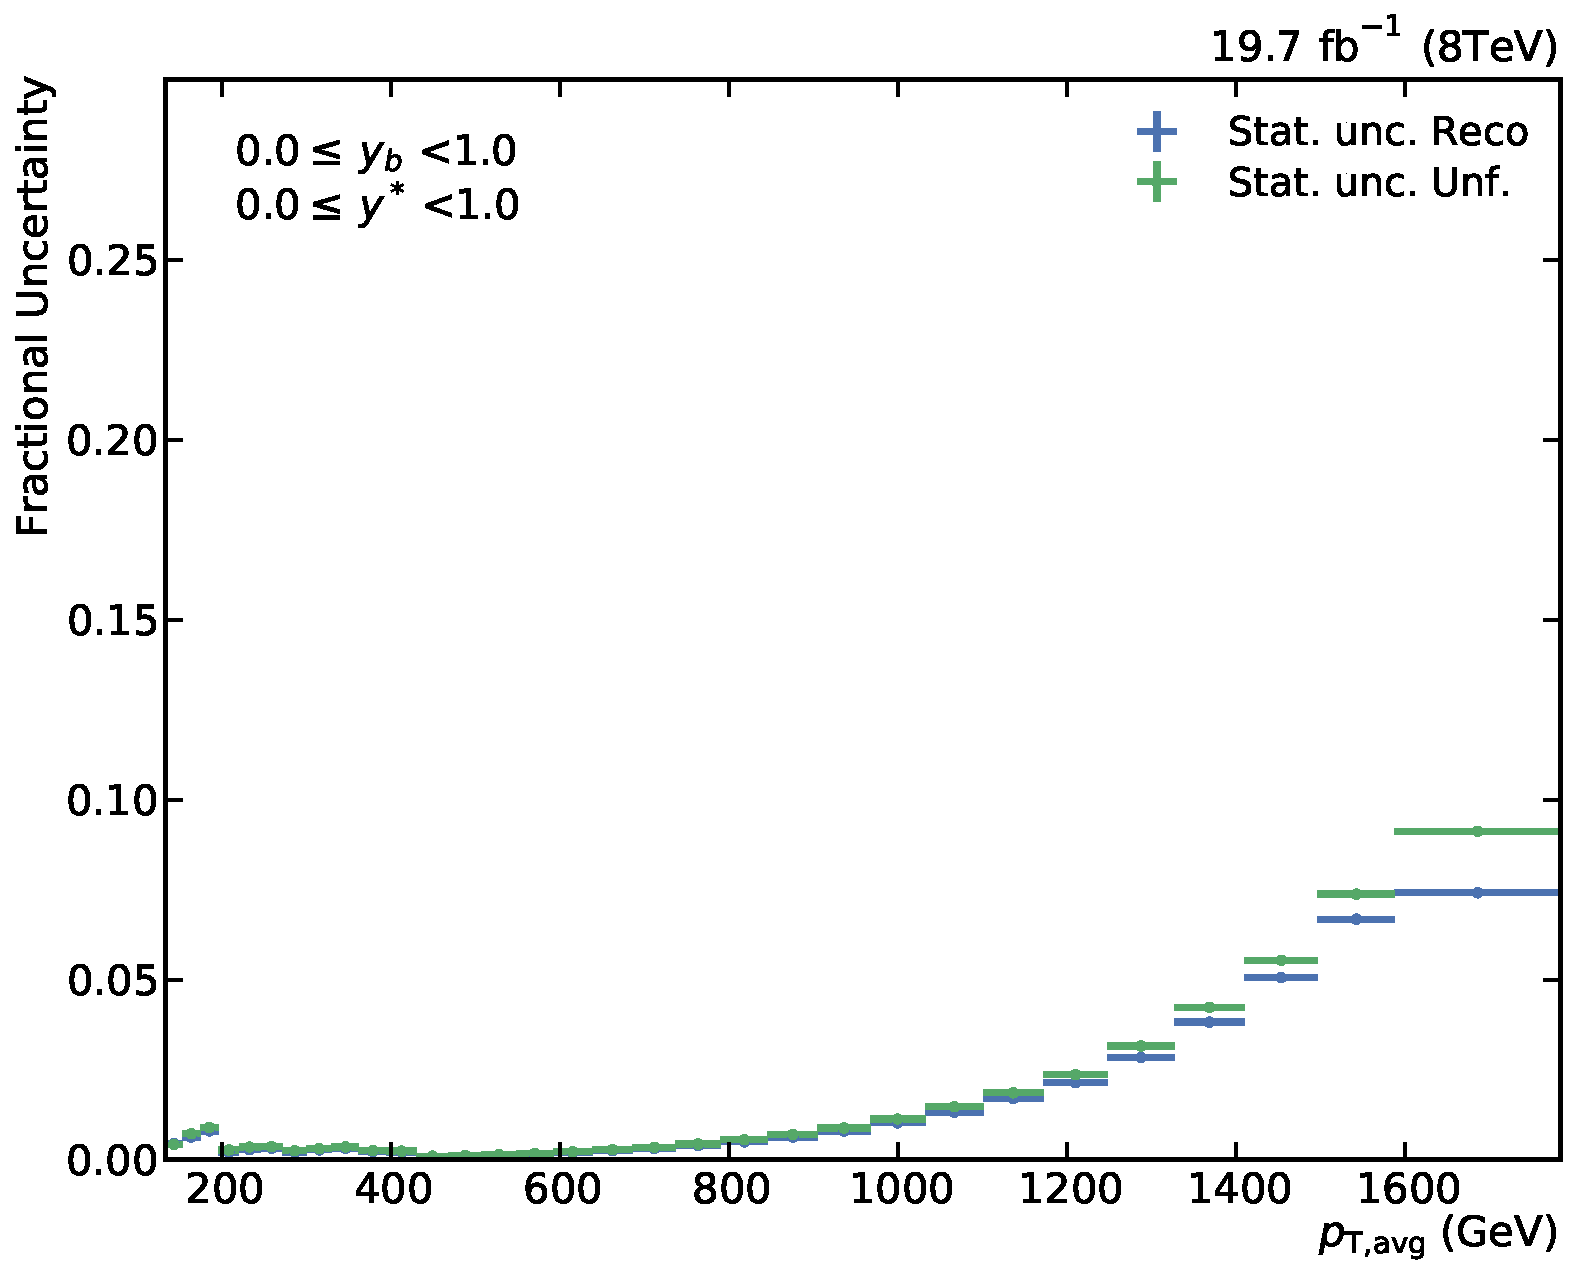
\includegraphics[width=0.45\textwidth]{figures/measurement/statunc_fractional_yb0ys0.pdf}\hfill
    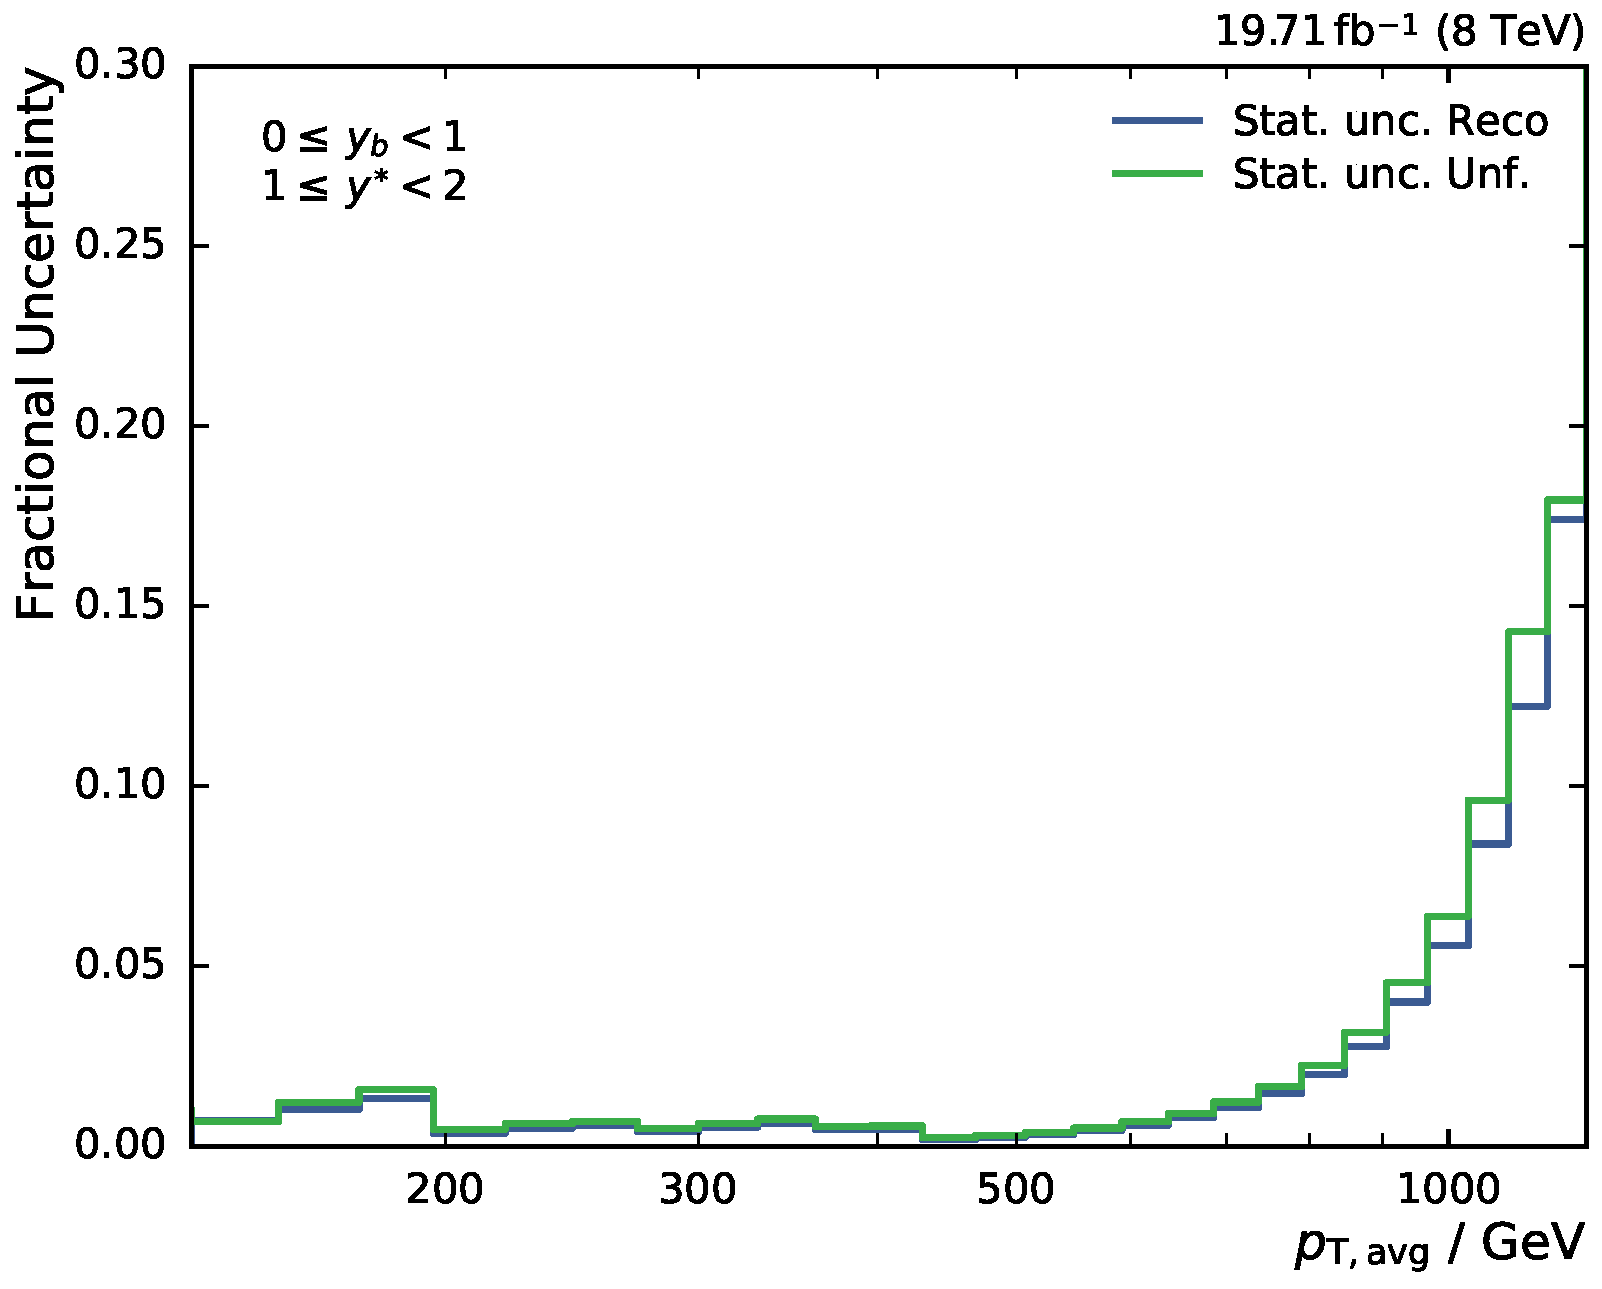
\includegraphics[width=0.45\textwidth]{figures/measurement/statunc_fractional_yb0ys1.pdf}
    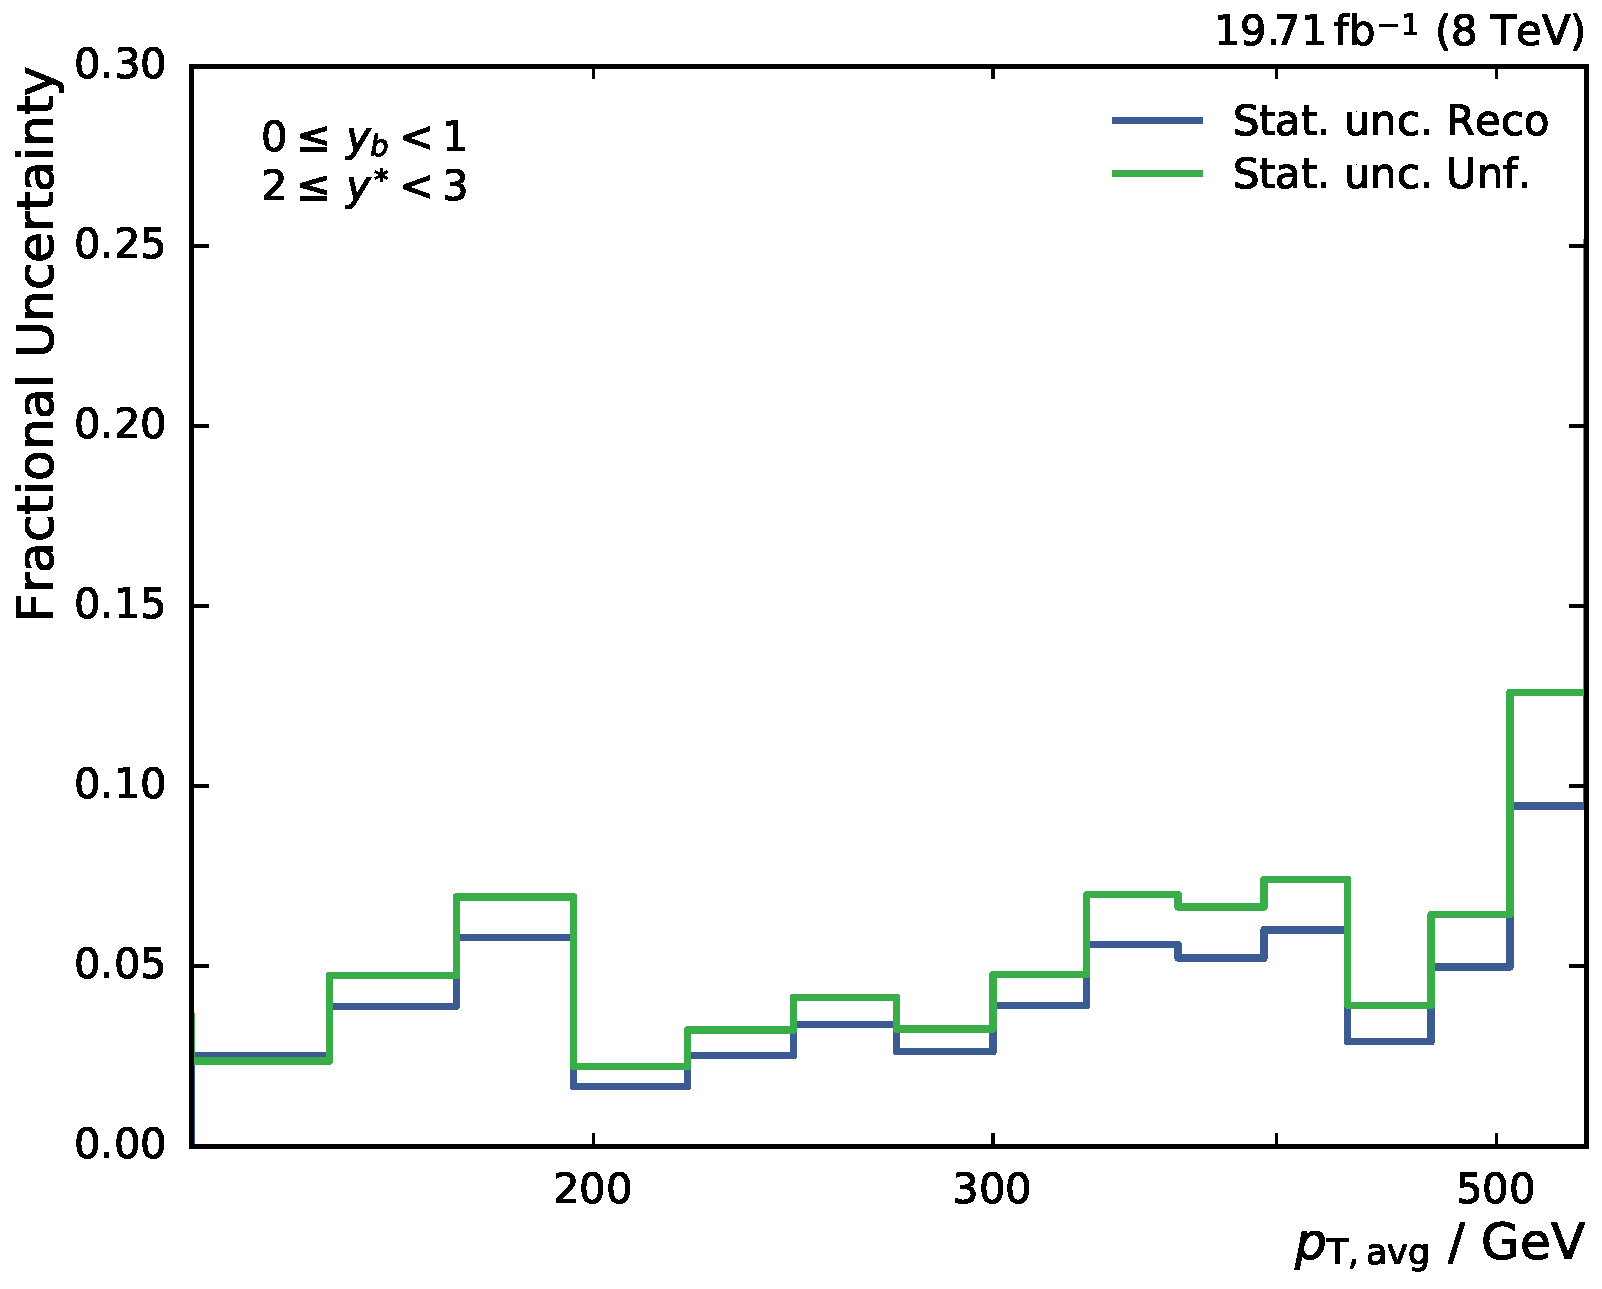
\includegraphics[width=0.45\textwidth]{figures/measurement/statunc_fractional_yb0ys2.pdf}\hfill
    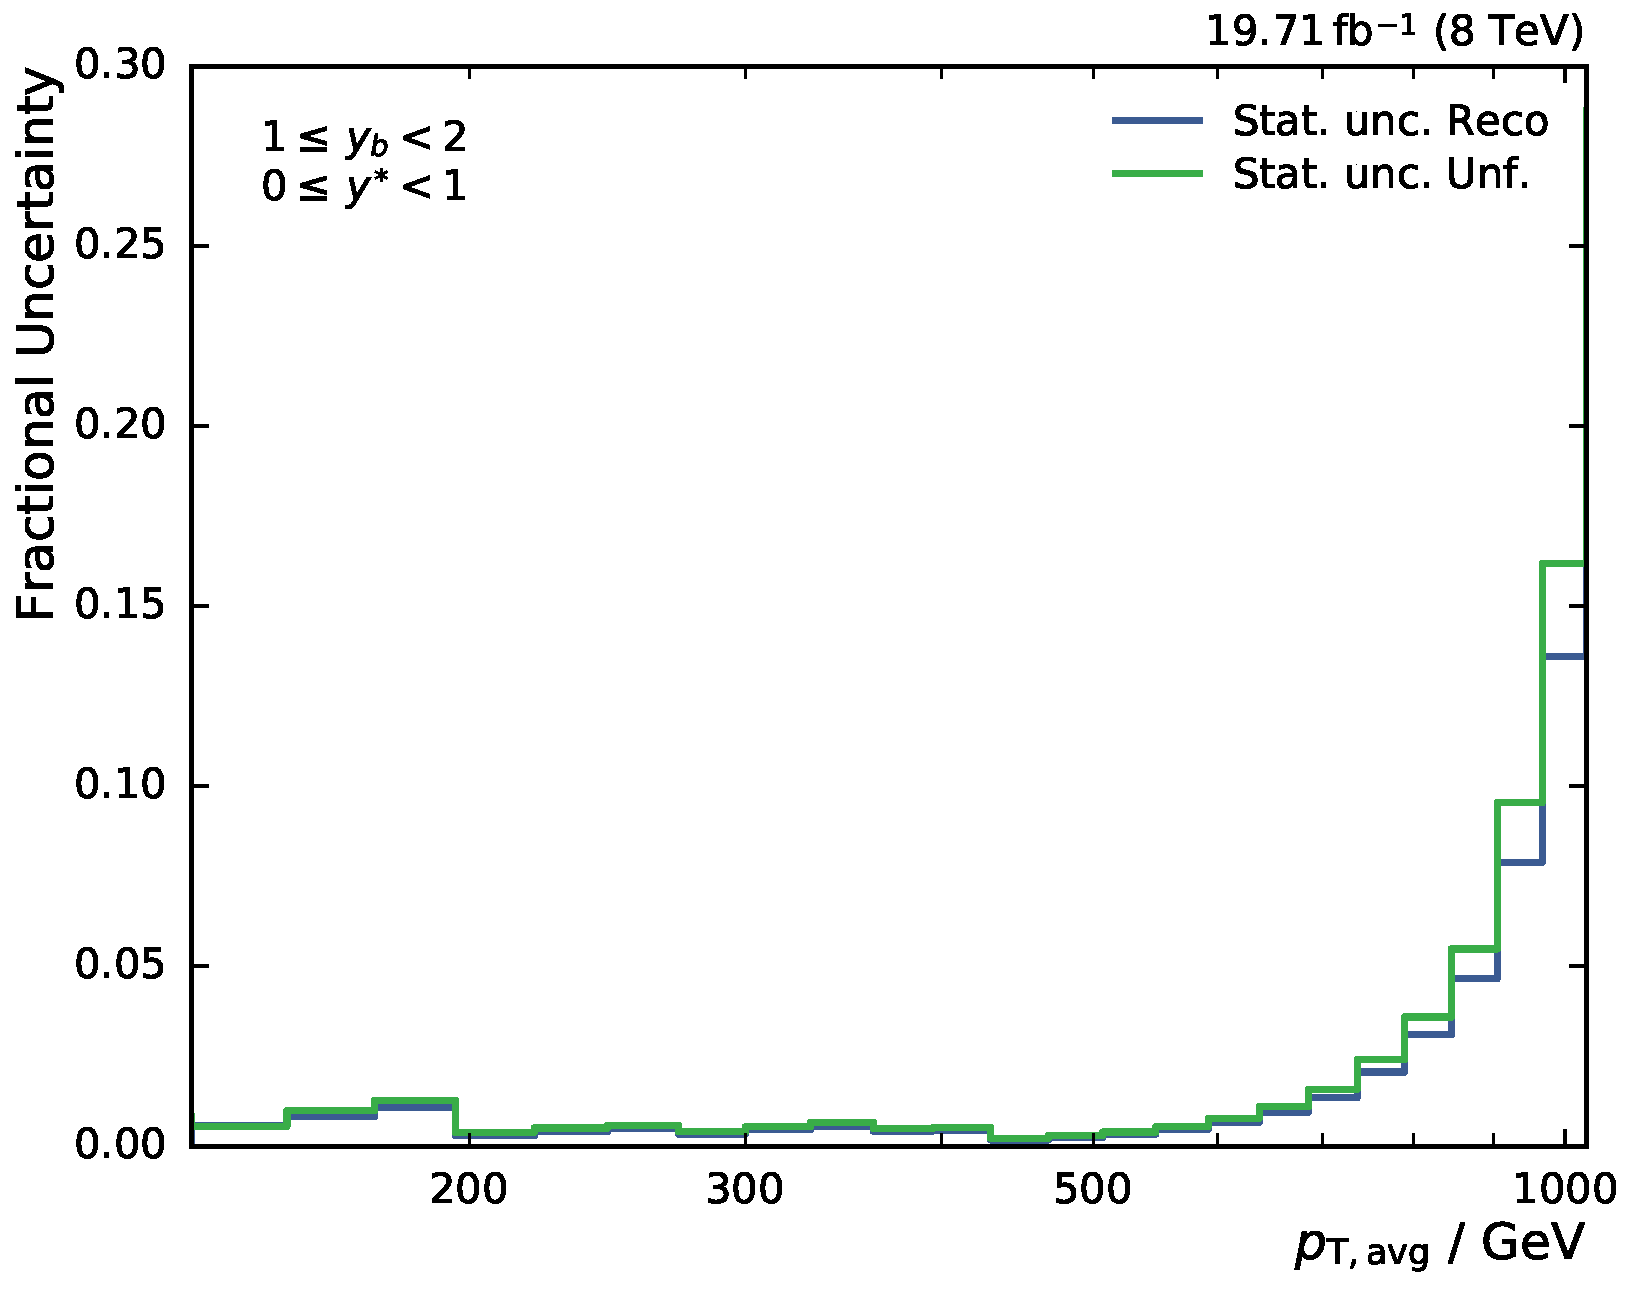
\includegraphics[width=0.45\textwidth]{figures/measurement/statunc_fractional_yb1ys0.pdf}
    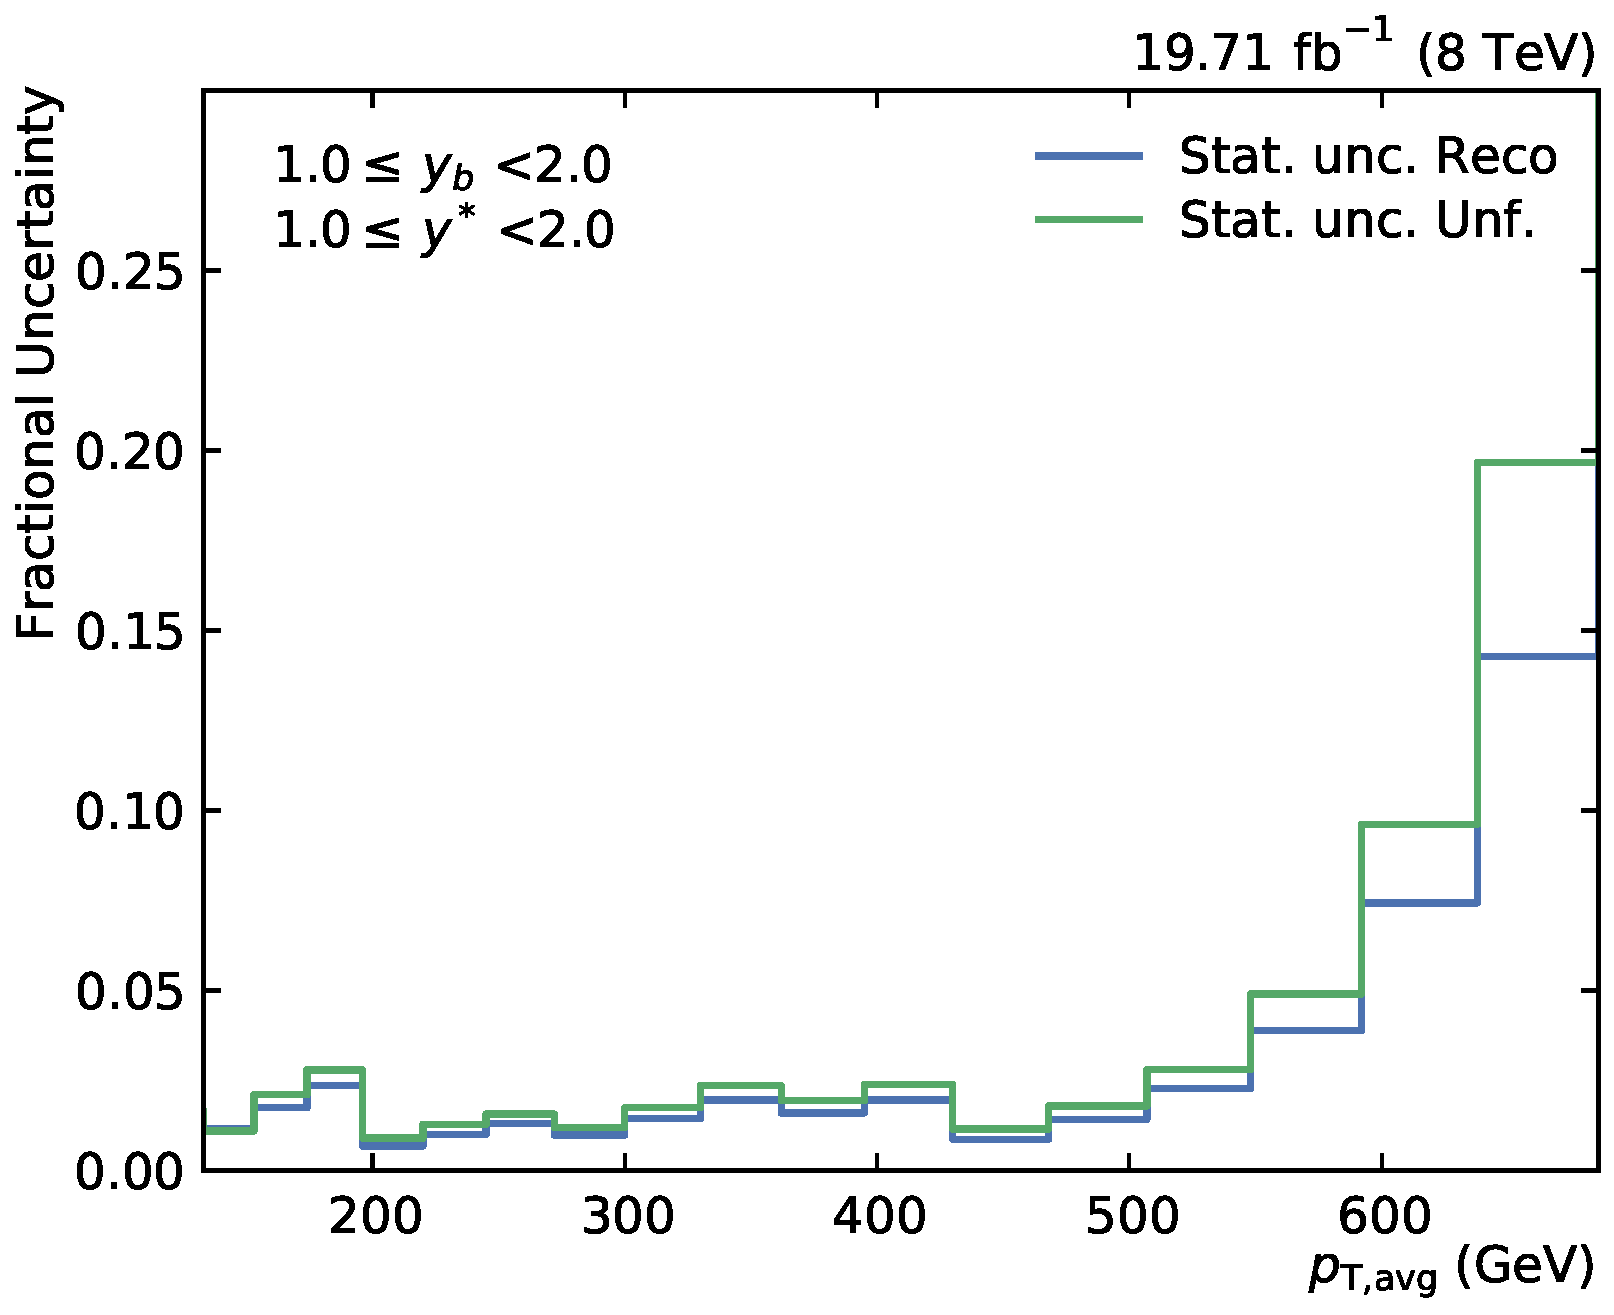
\includegraphics[width=0.45\textwidth]{figures/measurement/statunc_fractional_yb1ys1.pdf}\hfill
    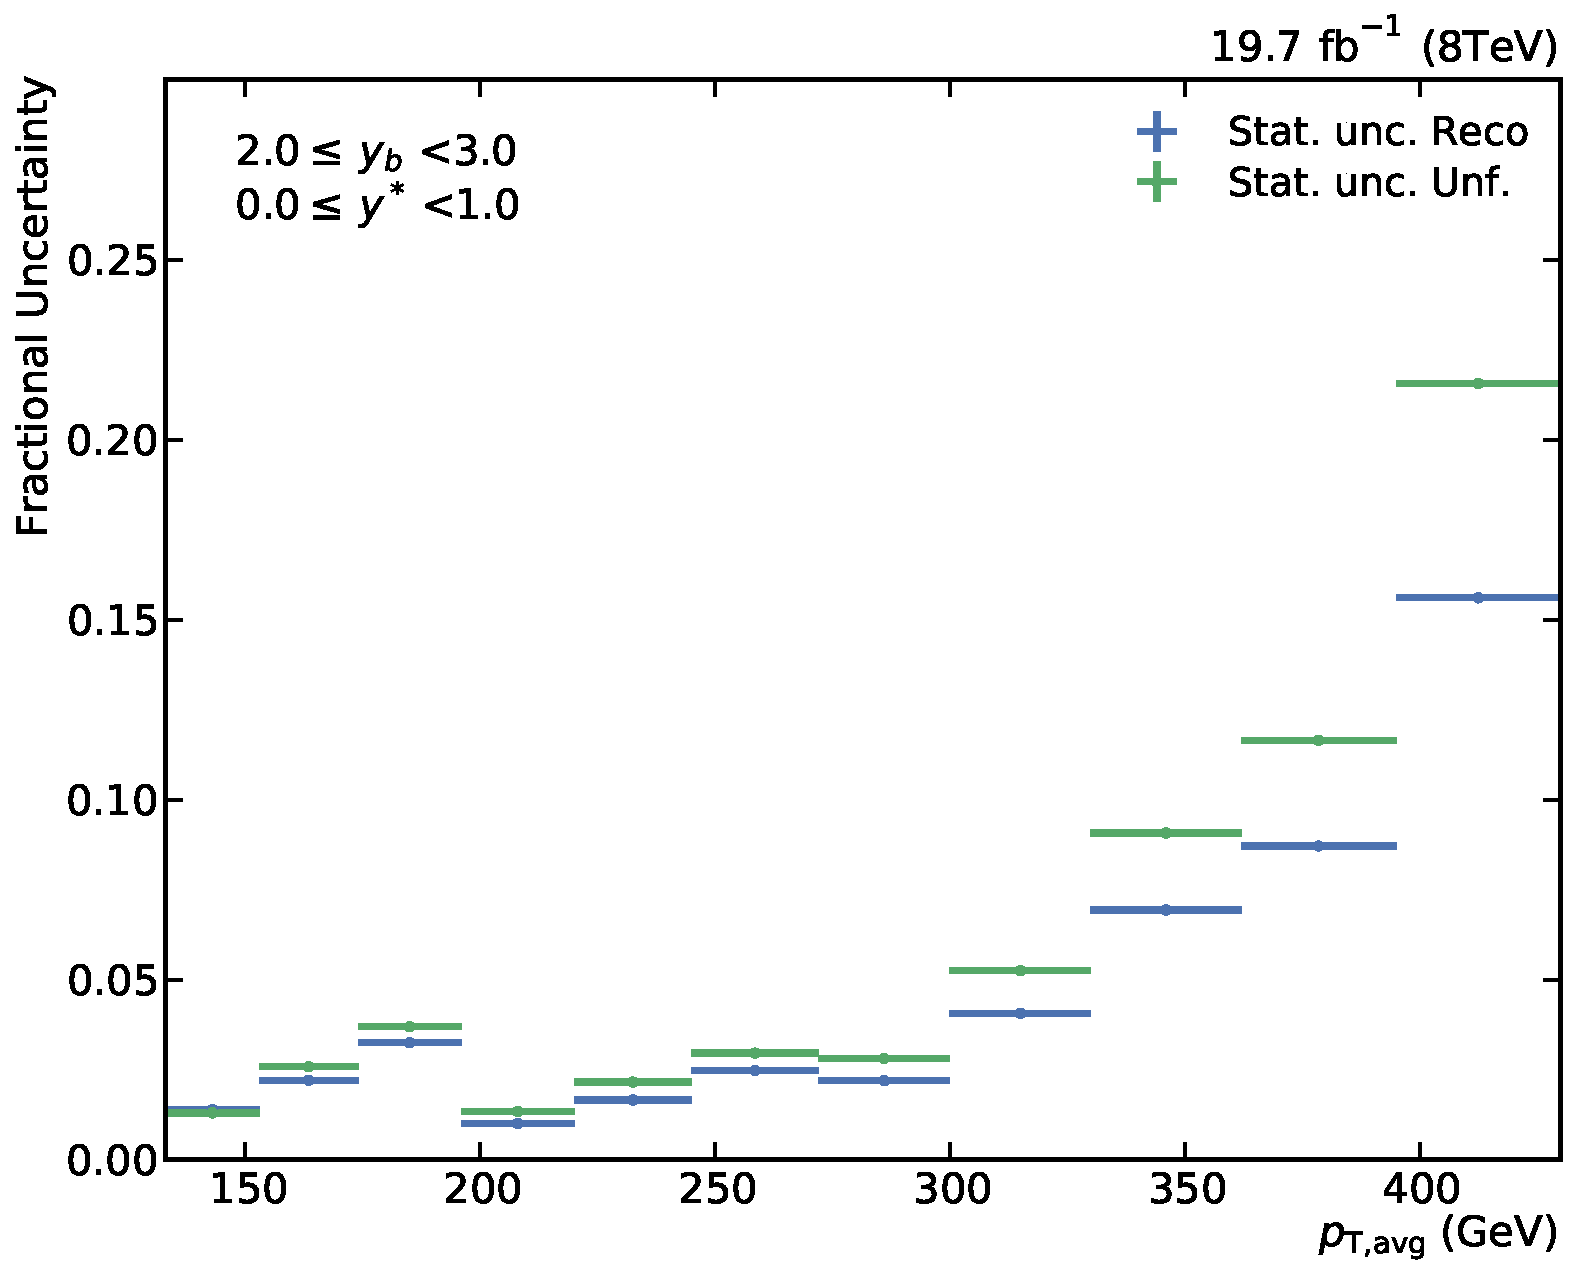
\includegraphics[width=0.45\textwidth]{figures/measurement/statunc_fractional_yb2ys0.pdf}
    \caption{The statistical uncertainties of the measured and the unfolded spectrum. Due
    to the unfolding procedure, the uncertainties slightly increase compared to the
    measured spectrum.}
    \label{fig:statunc_relative}
\end{figure}

Futhermore, the unfolding introduces a correlation between bins due to bin
migrations. These correlations are significant for neighbouring bins in \pt and
negligible for far off bins. Figure~\ref{fig:corr_unfolding_nlo} shows the
correlations of the statistical uncertainty after the unfolding.

\begin{figure}[htbp]
    \centering
    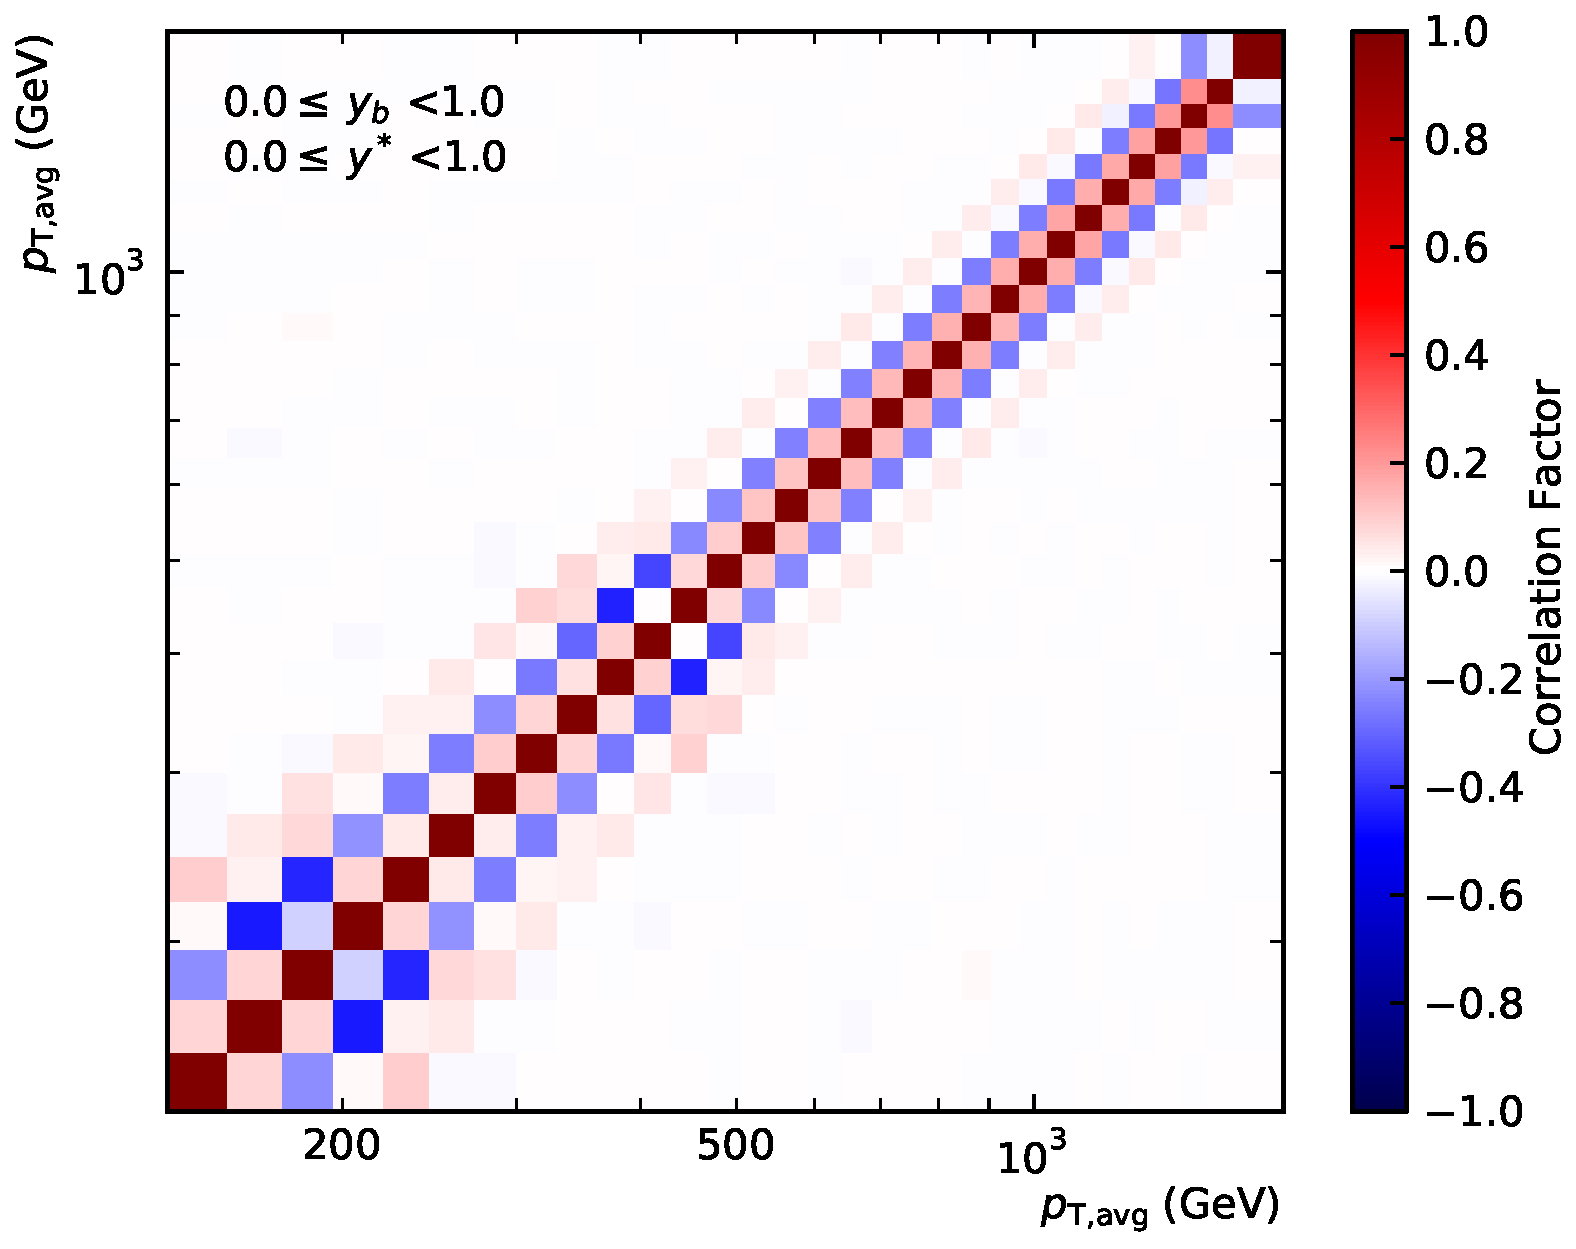
\includegraphics[width=0.45\textwidth]{figures/measurement/unf_nlo_corr_yb0ys0.pdf}\hfill
    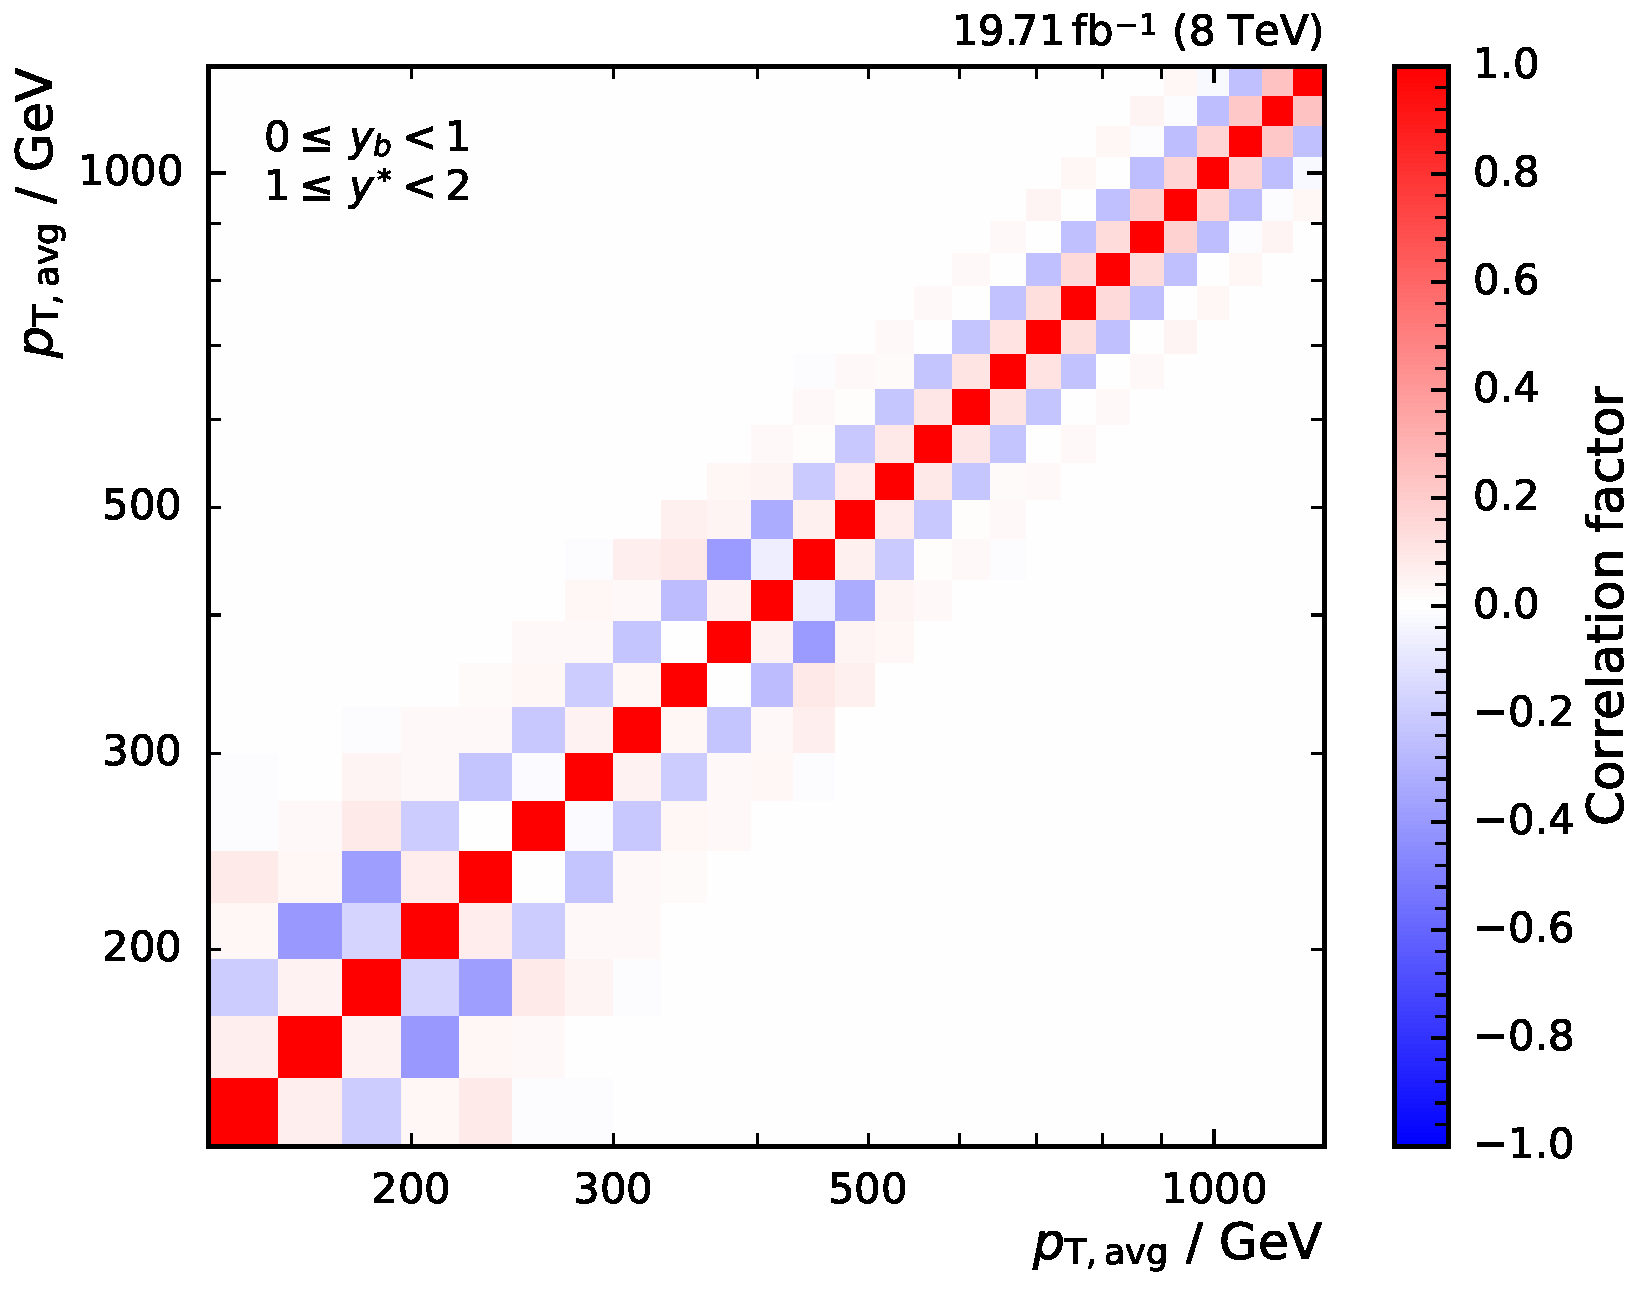
\includegraphics[width=0.45\textwidth]{figures/measurement/unf_nlo_corr_yb0ys1.pdf}
    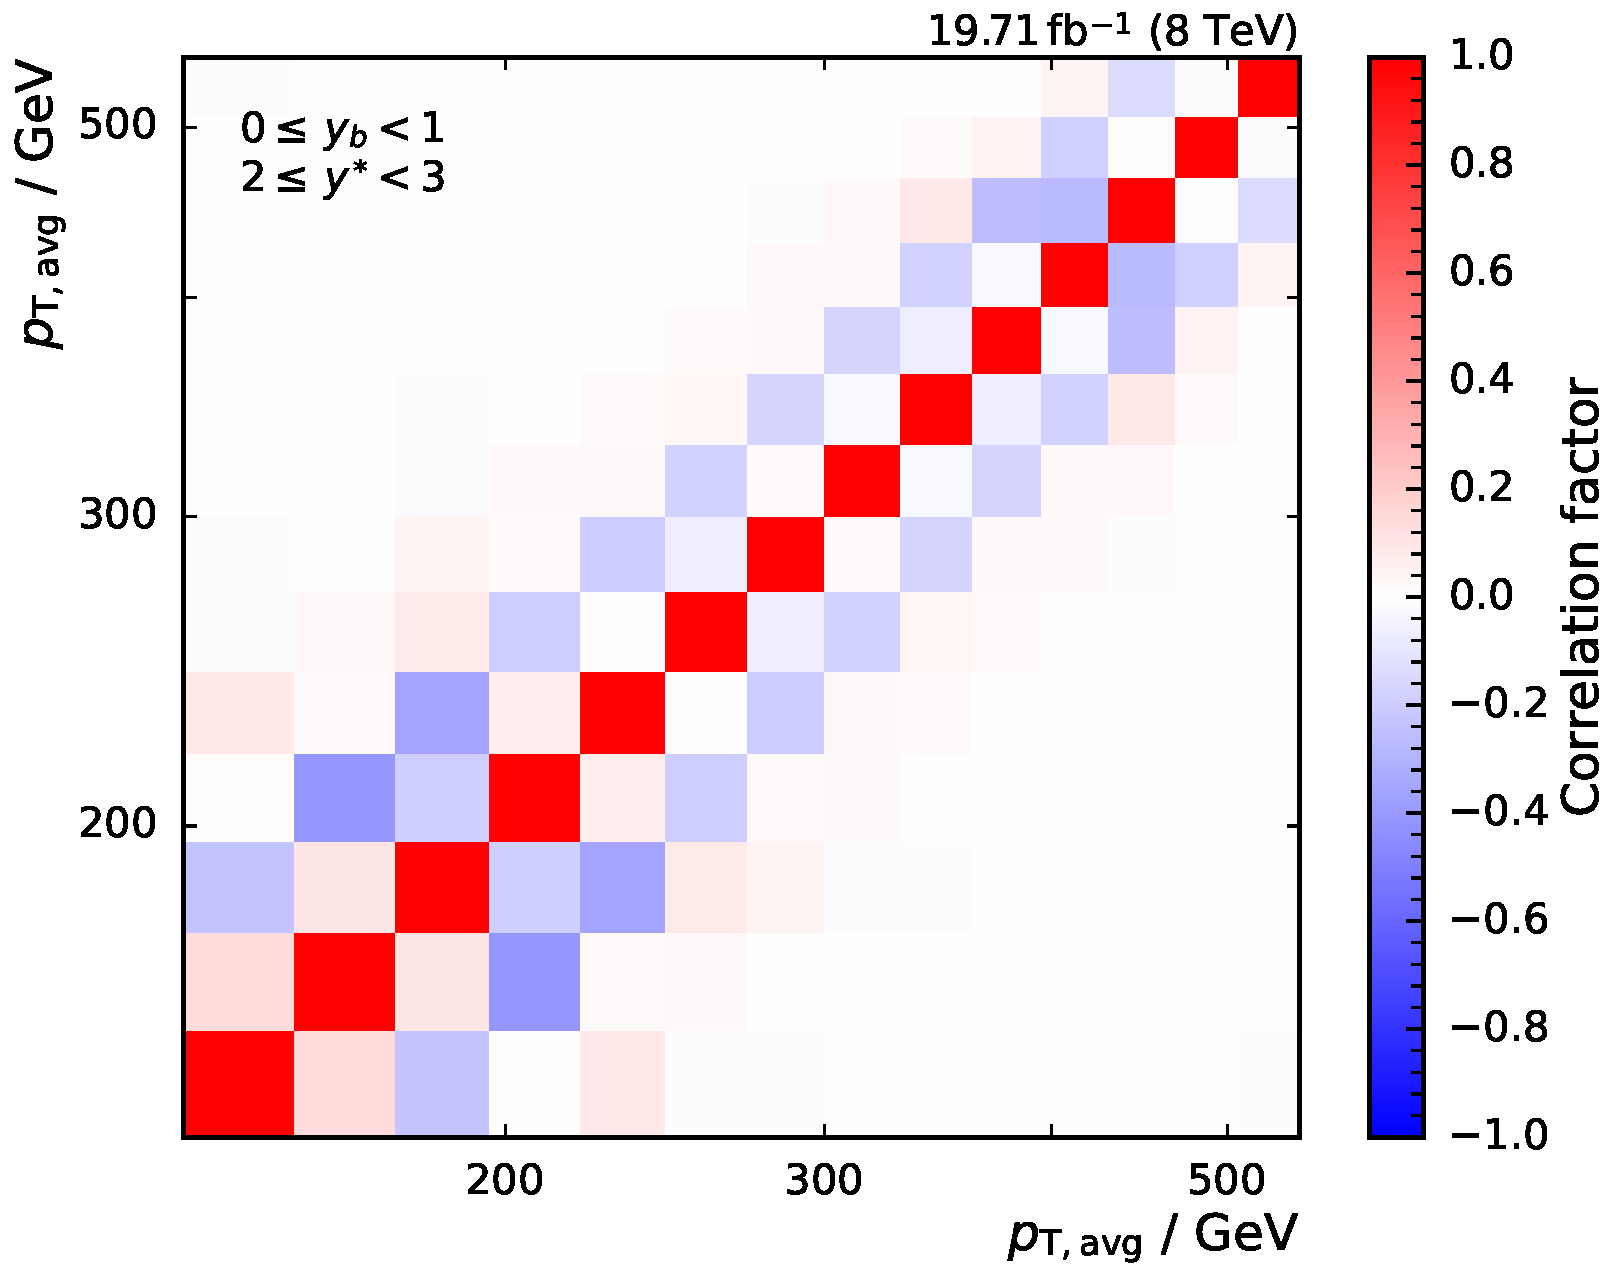
\includegraphics[width=0.45\textwidth]{figures/measurement/unf_nlo_corr_yb0ys2.pdf}\hfill
    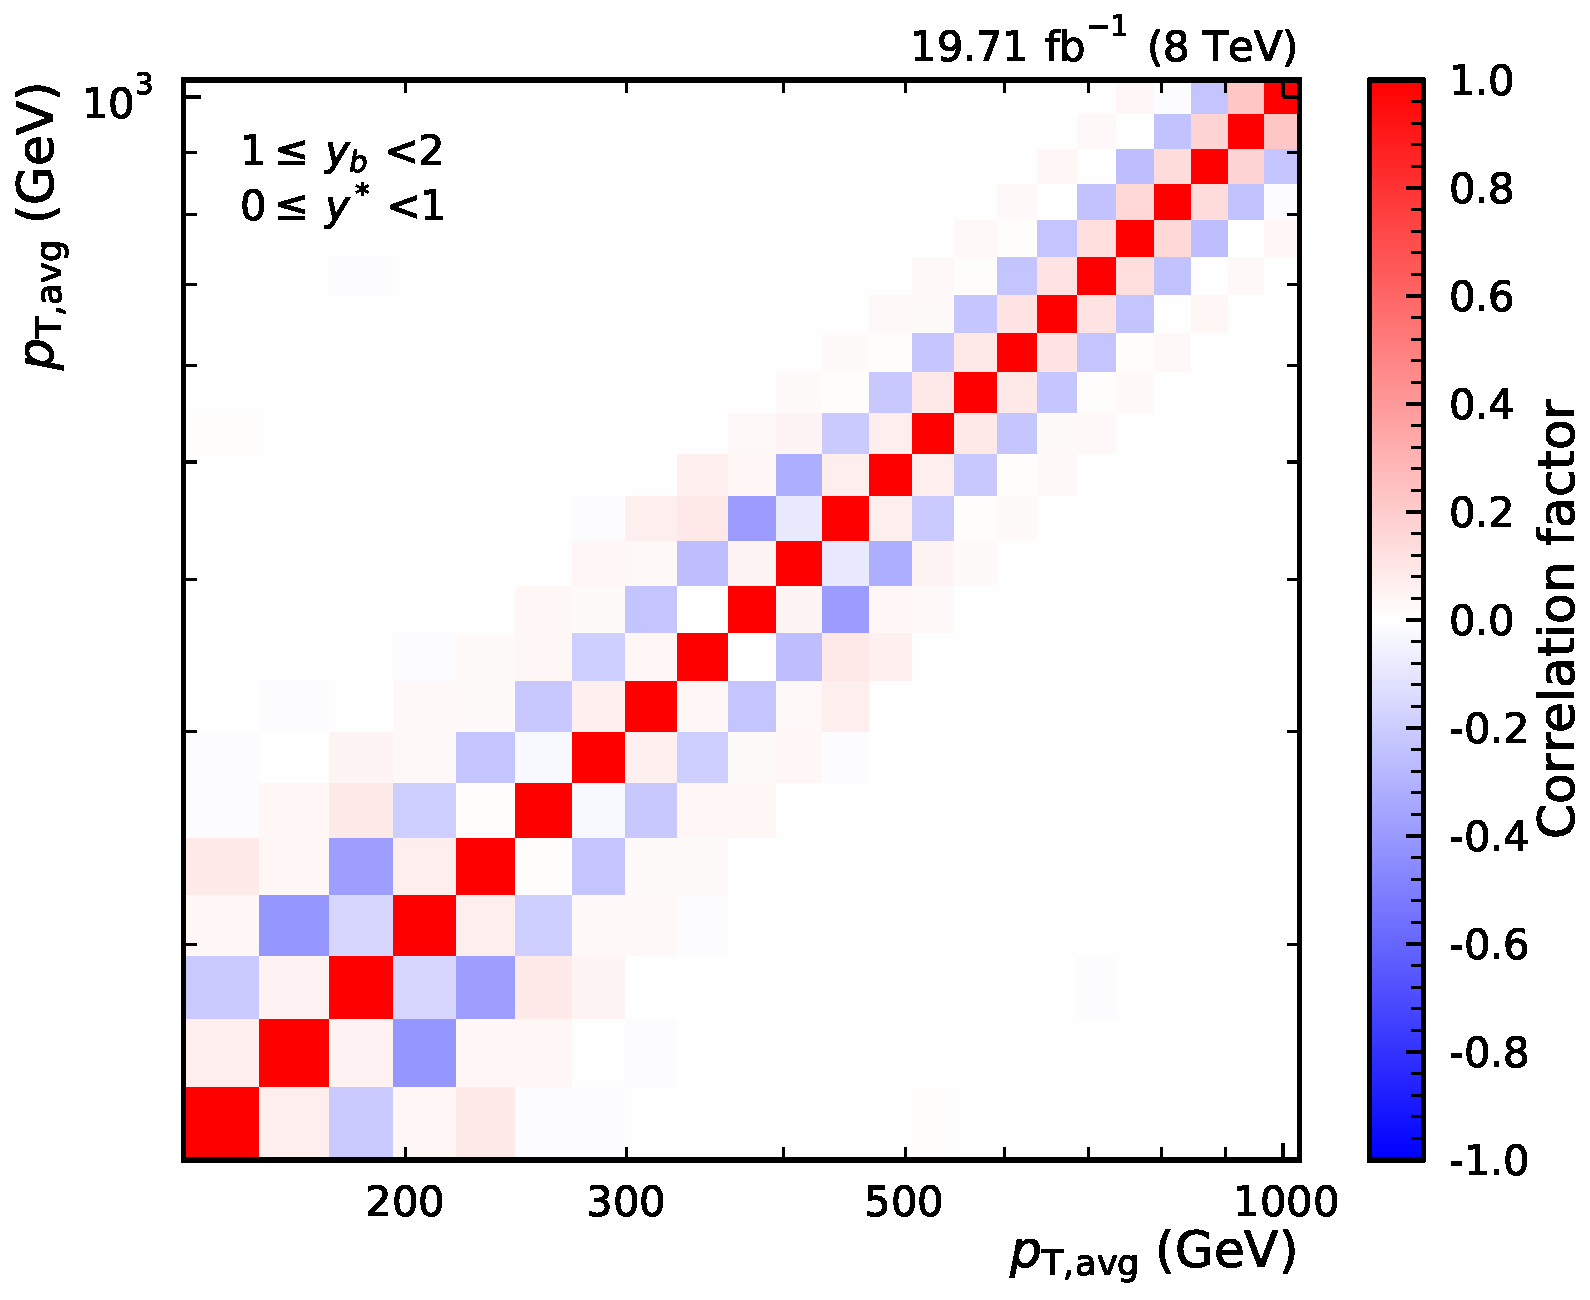
\includegraphics[width=0.45\textwidth]{figures/measurement/unf_nlo_corr_yb1ys0.pdf}
    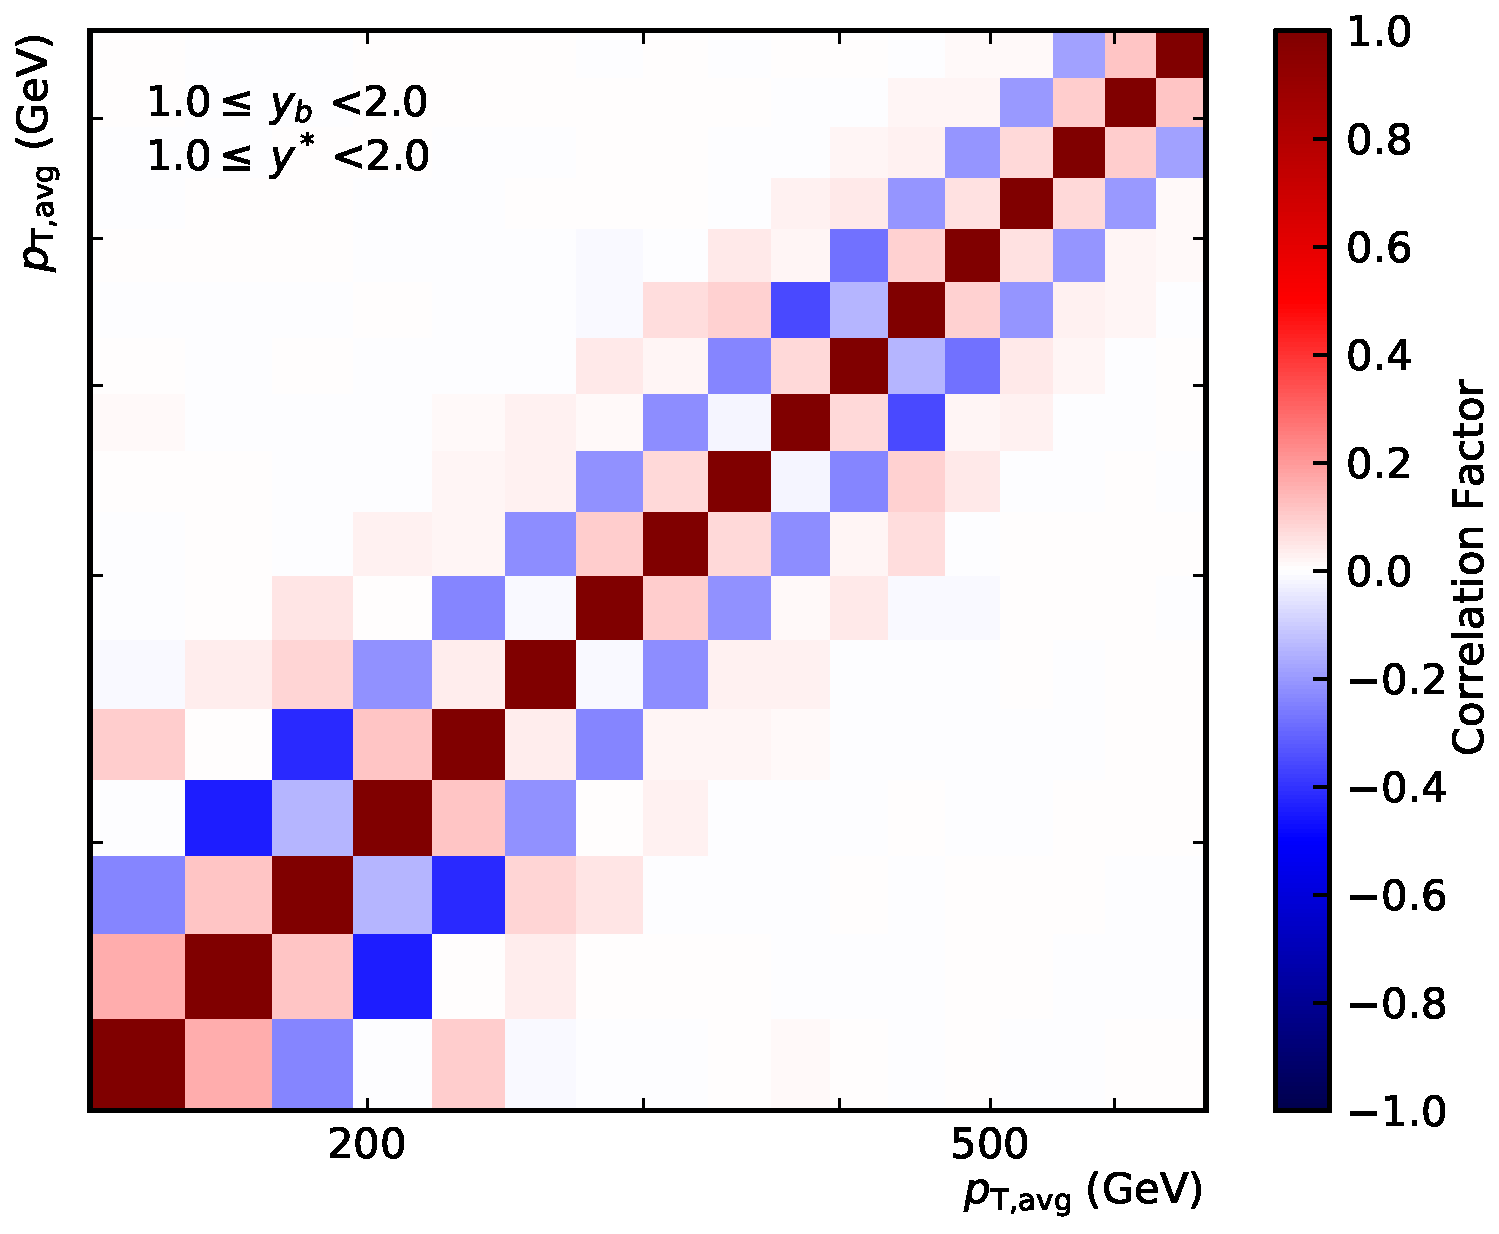
\includegraphics[width=0.45\textwidth]{figures/measurement/unf_nlo_corr_yb1ys1.pdf}\hfill
    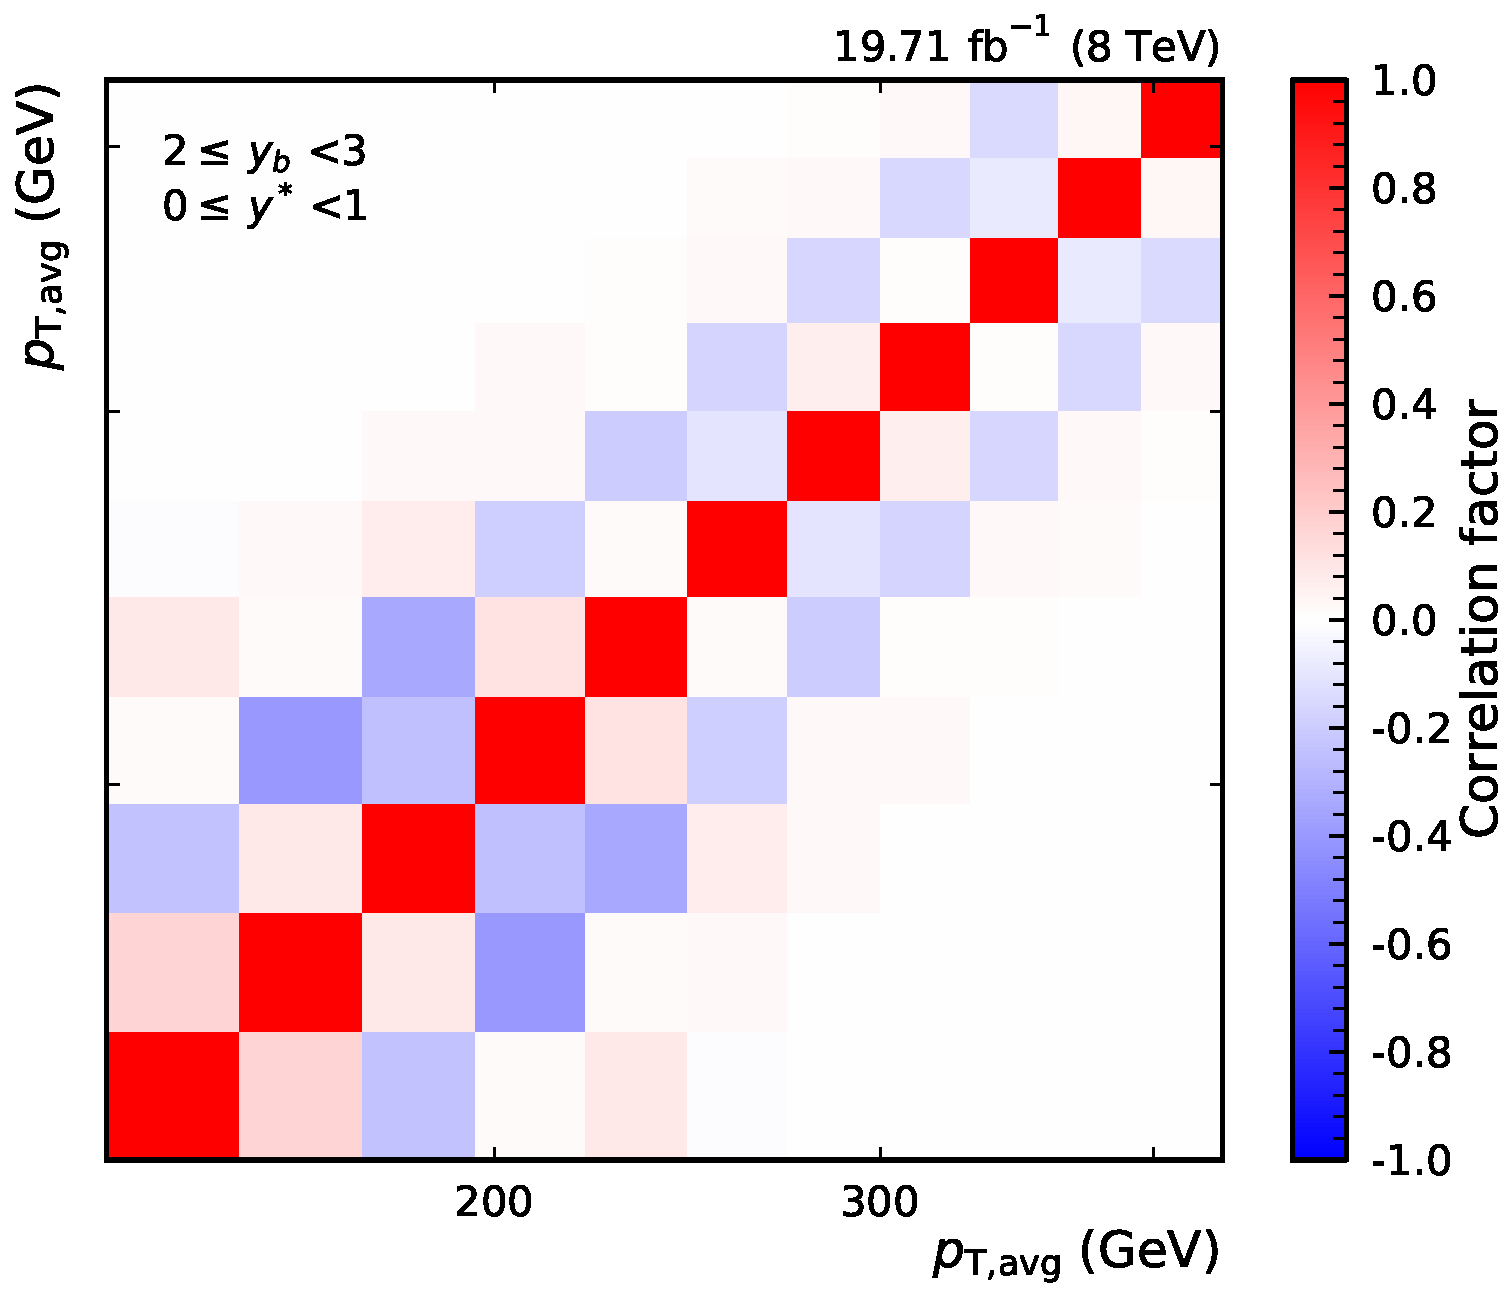
\includegraphics[width=0.45\textwidth]{figures/measurement/unf_nlo_corr_yb2ys0.pdf}
    \caption{Statistical correlations after the unfolding procedure. Close-by bins in \ptavg
    have a non-negligible correlation after the unfolding prodecure due to bin-by-bin migrations.}
    \label{fig:corr_unfolding_nlo}
\end{figure}

\subsection{Jet Energy Correction Uncertainty}

The dominant part of the experimental uncertainties comes from jet energy
calibration, which correct the measured jet energy for a variety of detector
effects, see Sec.~\ref{sec:jec}. As the corrections are afflicted with multiple
sources of systematic uncertainty, these are propgated individually to the cross section
measurement to conserve all correlations.

The JEC uncertainties are split into 25 mutually independent sources of
uncertainty (JES), in which each source is fully correlated in \pt and $\eta$
and presents a $1\sigma$ shift. As these uncertainties can be asymmetric, the
upwards and downwards variation are treated separately. The sum in quadrature of
all uncertainty sources equals the total uncertainty. Therefore they can be
treated exactly like the PDF eigenvectors sets, which were discussed in
Sec.~\ref{sec:pdf_uncertainties}. The sources of uncertainties are grouped in
four categories which relate to the underlying correction. In the following
list, a short summary of the sources of uncertainty is given. The calibration
procedure and the uncertainties are described in great detail
in~\ref{jec_paper}.

\begin{description}
    \item[Pile-up JES] Differences in the transverse momentum between the true
        offset and the random cone offset observed in simulation. This
        difference is propagated using Z/$\gamma$+jet and dijet balancing
        methods to estimate the residual pileup uncertainty after the
        calibration.
    \item[Relative JES] The relative $\eta$-dependent corrections calibrate
        forward jets using balanced dijet events. The largest contribution to
        the uncertainty arises from jet energy resolution and soft-radiation
        bias corrections. 
    \item[Absolute JES]  The absolute calibration of the jet energy scale relies
        on Z/$\gamma$+jet and multijet events. The uncertainties are related to
        the lepton momentum scale for muon and the single-pion response in the
        HCAL. Observed differences in applied methods, traced back to neutrinos
        and ISR, are also accounted for. 
    \item[Flavor JES] Differences in the flavor response are studied using
        simulation by cross-checking the results with quark- and gluon-tagged
        photon+jet and Z+jet events. The uncertainty is derived based on
        differences observed in the Pythia6 and Herwig++ simulation.
\end{description}

\subsection{Jet Energy Resolution Uncertainty}

\section{Comparison with NLO Predictions}

\begin{figure}[htbp]
    \centering
    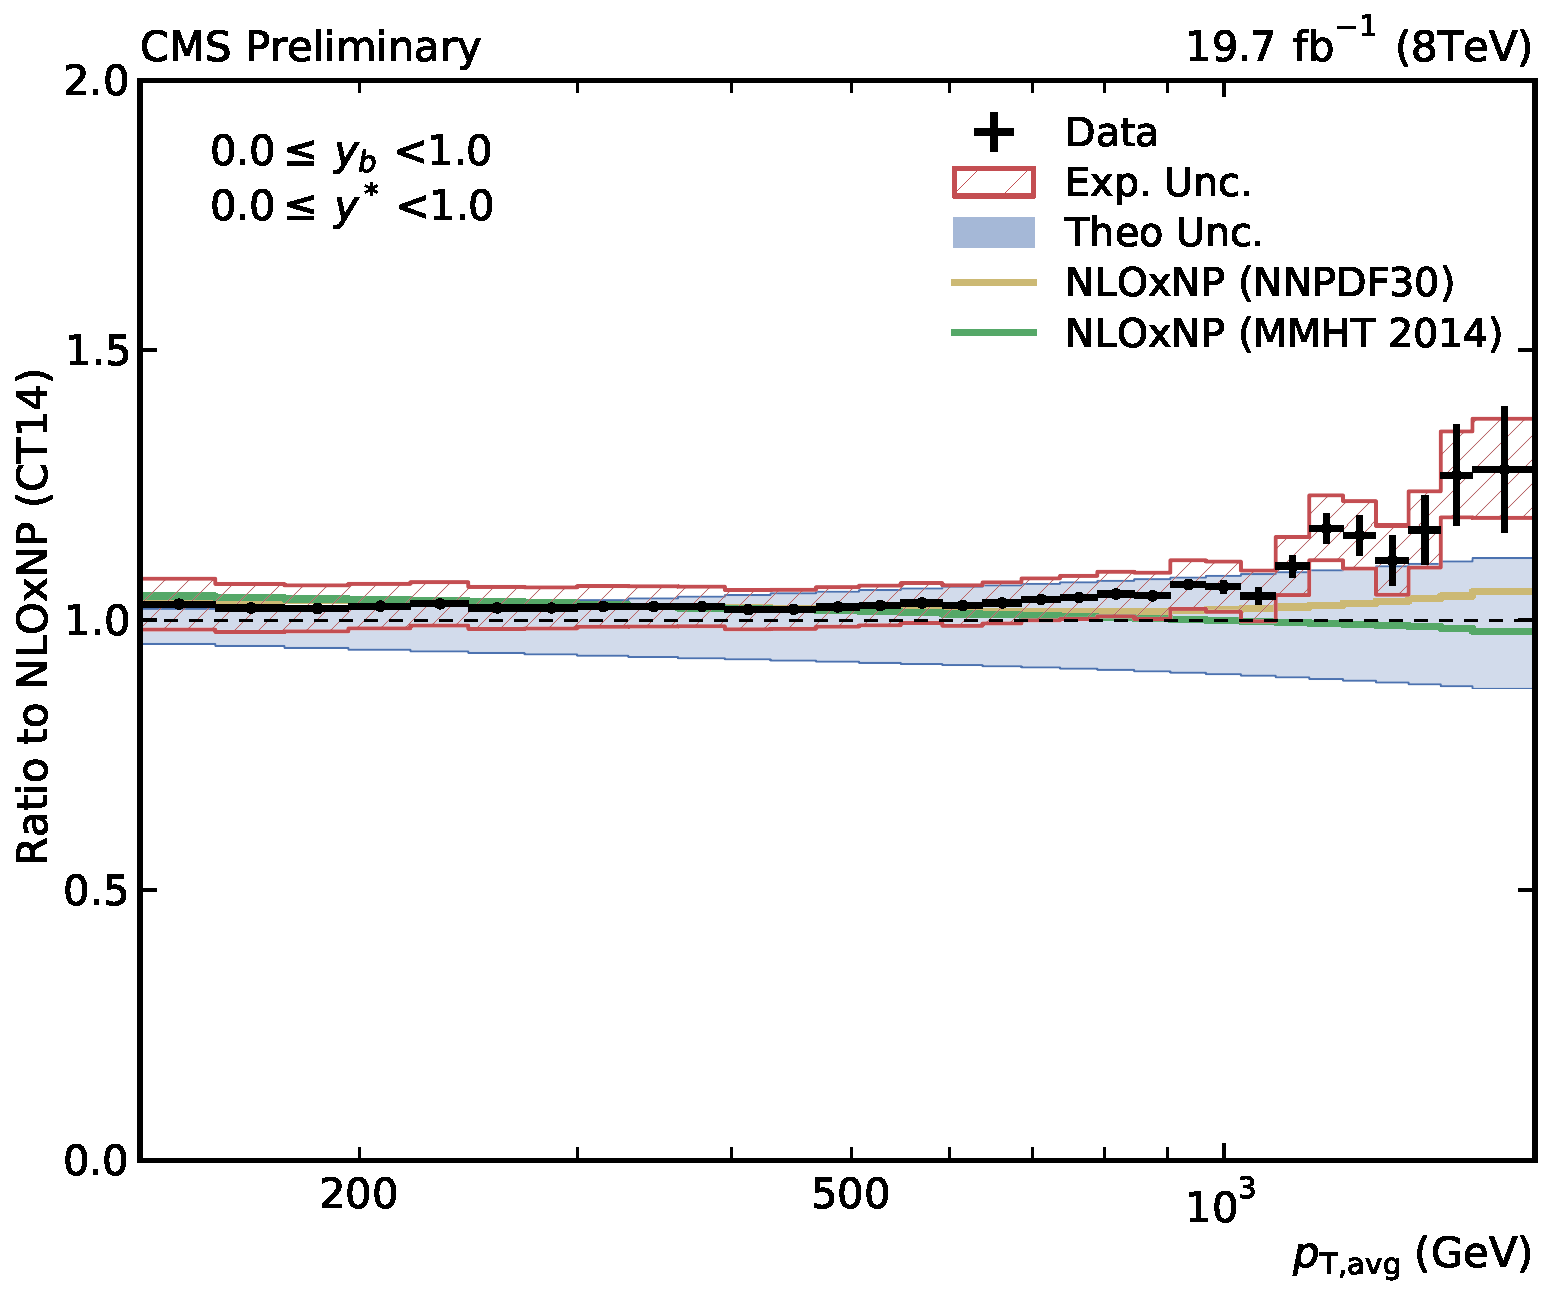
\includegraphics[width=0.45\textwidth]{figures/measurement/ratio_to_Ct14nlo+np_totcomp_yb0ys0.pdf}\hfill
    \includegraphics[width=0.45\textwidth]{figures/measurement/ratio_to_Ct14nlo+np_totcomp_yb0ys1.pdf}
    \includegraphics[width=0.45\textwidth]{figures/measurement/ratio_to_Ct14nlo+np_totcomp_yb0ys2.pdf}\hfill
    \includegraphics[width=0.45\textwidth]{figures/measurement/ratio_to_Ct14nlo+np_totcomp_yb1ys0.pdf}
    \includegraphics[width=0.45\textwidth]{figures/measurement/ratio_to_Ct14nlo+np_totcomp_yb1ys1.pdf}\hfill
    \includegraphics[width=0.45\textwidth]{figures/measurement/ratio_to_Ct14nlo+np_totcomp_yb2ys0.pdf}
    \caption[]{}
    \label{fig:ratio_ct10_nlo}
\end{figure}


\label{sec:nlo_comparisons}
